% 预览源文件

%% LyX 2.5.0 created this file.  For more info, see https://www.lyx.org/.
%% Do not edit unless you really know what you are doing.
\documentclass[english,a4paper,12pt,reqno]{amsart}
\usepackage{tgtermes}
\usepackage[T1]{fontenc}
\usepackage{textcomp}
\usepackage[utf8]{inputenc}
\usepackage{xcolor}
\usepackage{babel}
\usepackage{verbatim}
\usepackage{mathrsfs}
\usepackage{mathtools}
\usepackage{amstext}
\usepackage{amsthm}
\usepackage{amssymb}
\usepackage{graphicx}
\usepackage{esint}
\usepackage[bookmarks=true,bookmarksnumbered=true,bookmarksopen=true,bookmarksopenlevel=3,
 breaklinks=true,pdfborder={0 0 0},pdfborderstyle={},backref=false,colorlinks=true]
 {hyperref}
\hypersetup{
 bookmarksdepth=3,linkcolor=red,citecolor=blue}

\makeatletter
%%%%%%%%%%%%%%%%%%%%%%%%%%%%%% Textclass specific LaTeX commands.
\numberwithin{equation}{section}
\numberwithin{figure}{section}

%%%%%%%%%%%%%%%%%%%%%%%%%%%%%% User specified LaTeX commands.
%\usepackage[all]{xy}
\usepackage{tikz-cd}
\usepackage[twoside,inner=1.3in,outer=1in,top=1in,bottom=1in]{geometry}
\usepackage{csquotes}

% 定义两个安全的局部深度切换命令，专门供 TOC 读取，不污染正文计数器
\DeclareRobustCommand{\skipsubsectionsinTOC}{\addtocontents{toc}{\protect\setcounter{tocdepth}{1}}}
\DeclareRobustCommand{\showsubsectionsinTOC}{\addtocontents{toc}{\protect\setcounter{tocdepth}{3}}} 
% 注：amsart 默认的最终深度通常是 3 (显示到 subsection)

\makeatother

\theoremstyle{plain}
\newtheorem{thm}{\protect\theoremname}
\newtheorem{prop}[thm]{\protect\propositionname}
\theoremstyle{remark}
\newtheorem{rem}[thm]{\protect\remarkname}
\theoremstyle{definition}
\newtheorem{defn}[thm]{\protect\definitionname}
\newtheorem{example}[thm]{\protect\examplename}
\theoremstyle{plain}
\newtheorem{lem}[thm]{\protect\lemmaname}
\usepackage[style=alphabetic,backref=true, isbn=false, url=false, doi=false, backend=biber]{biblatex}
\providecommand{\definitionname}{Definition}
\providecommand{\examplename}{Example}
\providecommand{\lemmaname}{Lemma}
\providecommand{\propositionname}{Proposition}
\providecommand{\remarkname}{Remark}
\providecommand{\theoremname}{Theorem}

\addbibresource{5@part1.bib}
\begin{document}
\title{Optimal Test Functions for K-unstable Toric Varieties and Secondary
Polytopes}
\author{Li Sheng}
\address{School of Mathematics, Sichuan University, Chengdu 610064, P. R. China.}
\email{lshengscu@gmail.com}
\author{Yi Yao}
\address{School of Mathematics, Hunan University, Changsha 410082, P. R. China.}
\email{yeeyoe@163.com}
\begin{abstract}
For K-unstable toric varieties, Székelyhidi's optimal test-function
$\Theta_{P}$ is a mysterious concave function over the moment polytope
$P$, which encodes the limit behavior of Calabi flow. This paper
aims to quantize $\Theta_{P}$ by the maximal destabilizers for Chow-stability.
We determine these destabilizers by a combinatorial object called
shortest GKZ vector, which is the least norm point on the secondary
polytope associated to the lattice point set $P\cap k^{-1}\mathbb{Z}^{n}$.
When the moment polytope is Delzant, we show that these maximal
Chow-destabilizers converge to $\Theta_{P}$ in $L^{2}$ as
$k\rightarrow\infty$, without any compactness assumption.
Under a $C^{0}$-precompactness assumption the convergence is uniform.
It may provide an algorithm to detect K-unstability of toric varieties.
\end{abstract}

\maketitle
\global\long\def\lam{\lambda}%
 
\global\long\def\vphi{\varphi}%
 
\global\long\def\cch{\mathcal{H}}%
 
\global\long\def\bbc{\mathbb{C}}%
 
\global\long\def\bbcs{\mathbb{C}^{*}}%
 
\global\long\def\bbr{\mathbb{R}}%
 
\global\long\def\bbz{\mathbb{Z}}%
 
\global\long\def\bbn{\mathbb{N}}%

\global\long\def\ra{\rightarrow}%
 
\global\long\def\lead{\leadsto}%
 
\global\long\def\bdot{\bm{\cdot}}%
 
\global\long\def\'{\prime}%
 
\global\long\def\cleq{\preceq}%
\global\long\def\cgeq{\succeq}%
 
\global\long\def\na{{\scriptscriptstyle \mathsf{NA}}}%
 
\global\long\def\an{\mathrm{an}}%
 
\global\long\def\ma{\mathrm{MA}}%

\tableofcontents{}

\section{Introduction}

\skipsubsectionsinTOC

Consider a seemingly innocent variational problem. Let $P$ be a full-dimensional
polytope in $\bbr^{n}$, one wants to minimize the functional 
\begin{equation}
\Psi(\eta)=\frac{1}{2}\int_{P}\eta^{2}\mathrm{d}x+\int_{\partial P}\eta\ \mathrm{d}\sigma,\ \eta:P\rightarrow\bbr\text{ is convex},\label{eq: begin Phi}
\end{equation}
where $\mathrm{d}x$ is Lebesgue measure and boundary measure $\mathrm{d}\sigma$
is proportional to the Lebesgue measure on each facet. If one decreases
the boundary integral, convexity will force the $L^{2}$-norm to increase.
Indeed, $\Psi$ admits a unique minimizer $f^{*}$. In most situations,
$f^{*}$ is affine. It remains unknown whether $f^{*}$ is always
piecewise affine and how to determine it numerically. 

This variational problem originates from Székelyhidi \cite{szekelyhidi_optimal_2008}.
Its minimizer relates to the long-time behavior of the Calabi flow
on the toric Kähler manifold associated to $P$. We discuss this context
below.

Let $(X,L)$ be the polarized toric Kähler manifold induced by a lattice
Delzant polytope $P\subset M_{\bbr}\coloneqq M\otimes\bbr$, where
$M$ is a lattice of rank $n$. As an instance of Yau--Tian--Donaldson
conjecture, the existence of extremal metrics in class $c_{1}(L)$
is expected to be equivalent to a stability condition on $P$, see
\cite{donaldson_scalar_2002,szekelyhidi_introduction_2014}. With
the aid of torus symmetry, the existence can be reduced to the solvability
of a fourth-order PDE on $P$. The stability condition is called the
relative K-polystability, which requires that the relative Donaldson--Futaki
invariant
\[
\mathbb{M}^{\mathrm{rel}}_{P}(\eta)\coloneqq\int_{\partial P}\eta\ \mathrm{d}\sigma-\int_{P}\eta\ell_{P}\ \mathrm{d}x\geq0
\]
for all rational piecewise affine convex functions $\eta$, with equality
only for affine $\eta$. See §\ref{subsec:Szekelyhidi's-optimal-test}
for details. 

It is widely accepted that this stability condition needs to be strengthened
to make the equivalence hold. There are two kinds of strengthened
conditions: uniform K-stabilities \cite{dervan_uniform_2016} and
testing more functions \cite{szekelyhidi_filtrations_2015}. To date,
various versions of equivalence have been established, refer to \cites{donaldson_extremal_2008}{chen_extremal_2018}{chen_constant_2021-1}{hisamoto_stability_2020}{li_geodesic_2022}{li_extremal_2023}{jubert_yautiandonaldson_2023}{nitta_uniform_2021}
and their references. Meanwhile, there are partial criteria to verify
stability practically, see \cite{zhou_relative_2008,yotsutani_relative_2019}. 

\subsection*{Optimal test function $\Theta_{P}$}

The unstable case has received less attention, see \cites{wang_existence_2011}{wang_k-stability_2014}{sektnan_investigation_2018}{yotsutani_relative_2019}{araujo_calabi_2023}
for examples. When $P$ is relatively K-unstable (i.e. $\mathbb{M}^{\mathrm{rel}}_{P}$
may be negative), \cite{szekelyhidi_optimal_2008} showed the minimization
problem 
\[
\inf\left\{ \frac{\mathbb{M}^{\mathrm{rel}}_{P}(\eta)}{\left\Vert \eta\right\Vert _{2}}\ \Big|\ 0\neq\eta\in\mathcal{C}_{1}(P)\cap L^{2}(P)\right\} ,\ \left\Vert \eta\right\Vert ^{2}_{2}\coloneqq\int_{P}\eta^{2}\ \mathrm{d}x
\]
admits a unique minimizer $\ell_{P}-\Theta_{P}$ up to scaling, see
(\ref{eq:space C1}) for the enlarged space $\mathcal{C}_{1}(P)$
of convex functions. Proposition \ref{prop: recharac Theta} shows
that $-\Theta_{P}$ is actually the unique minimizer of $\Psi$ (\ref{eq: begin Phi})
above. Let $\Theta_{P}=\ell_{P}$ when $P$ is relatively K-semistable
(i.e. $\mathbb{M}^{\mathrm{rel}}_{P}\geq0$). We call this concave
function $\Theta_{P}$ ($=B$ in \cite{szekelyhidi_optimal_2008})
the \emph{optimal test function} for $P$. 

The boundedness of $\Theta_{P}$ is proved by Li, Lian and the first
author \cite{li_extremal_2023}. Repeat their proof, we find that
it can yield stronger results. 
\begin{thm}[\cite{li_extremal_2023} see §\ref{proof of Li-Lian-Sheng}]
\label{thm: theta is continuous-INTRO}  The optimal test function
$\Theta_{P}$ can extend to a concave function on the whole space.
In particular, $\Theta_{P}$ is continuous up to the boundary of $P$,
and the subdifferential set $\partial\left(-\Theta_{P}\right)\left(\mathrm{int}P\right)$
is bounded. 
\end{thm}

As \cite{szekelyhidi_optimal_2008} showed, $\Theta_{P}$ encodes
important information of $X$. For instance, if the Calabi flow admits
long-time solution, then the scalar curvature (as function on $P$)
would converge to $\Theta_{P}$. More interestingly, when $\Theta_{P}$
is piecewise affine, it induces a polyhedral decomposition of $P$,
then every subpolytope is semistable in a certain sense, see Theorem
\ref{thm: Gabor paper}. Hence $\Theta_{P}$ is analogous to the Harder--Narasimhan
filtration for the unstable holomorphic vector bundles, where the
monotonicity of the slopes of quotient bundles mimics the concavity
of $\Theta_{P}$. To the authors' knowledge, there is no explicit
example of $\Theta_{P}$ so far, see \cite{sektnan_investigation_2018}
for examples with zero boundary measure. By the way, the optimal test-functions
for Ding-stability of toric Fano varieties have been determined in
\cite{yao_mabuchi_2022}. They are always piecewise affine. 

\subsection*{Maximal destabilizers for K-stability}

Optimal test function $\Theta_{P}$ is a realization of maximal K-destabilizers
for general K-unstable Kähler manifold $(X,L)$. Recall that the constant
scalar curvature Kähler metrics are critical points of K-energy. When
$(X,L)$ is K-unstable, Xia \cite{xia_sharp_2021} show that there
is a unique (modulo parallel relation) finite-energy geodesic ray
along which the K-energy decreases fastest. By \cites{berman_variational_2021}{li_geodesic_2022},
this ray can be encoded into a non-Archimedean metric on $L$, which
we call the \emph{maximal K-destabilizer} of $(X,L)$. In the toric
setting, with the aid of symmetry, it reduces to $\Theta_{P}$, see
\cite[Example 44]{yao_maximal_2025}. 

\subsection*{Maximal destabilizers for Chow-stability}

The second author \cite{yao_maximal_2025} suggests to study the maximal
K-destabilizers via the Chow-stability. Since its birth in \cite{tian_kahler-einstein_1997},
K-stability has been closely connected with Chow-stability. Let $\iota_{k}:X\hookrightarrow\mathbb{P}R^{*}_{k}$
be the Kodaira embedding, where $R_{k}\coloneqq\mathrm{H}^{0}(X,kL)$.
Chow-stability means the GIT stability of Chow-form attached to $\iota_{k}(X)$.
Ross and Thomas \cite{ross_study_2006} showed that asymptotic Chow-semistability
can imply K-semistability. Hence if $(X,L)$ is K-unstable, then $(X,kL)$
is Chow-unstable for sufficiently large $k$. We can consider the
\emph{maximal Chow-destabilizer} for $\iota_{k}(X)$, which is defined
as a filtration on $R_{k}$ induced by the 1-ps of $\mathrm{SL}\left(R_{k}\right)$
minimizing the Chow-weights. 

A natural question is whether the maximal Chow-destabilizer converges
to the maximal K-destabilizer in a certain sense as $k\rightarrow\infty$.
This is similar to the stable case, in which Donaldson \cite{donaldson_scalar_2001}
used balanced metrics to approximate cscK metrics. One difference
is that there is no Euler--Lagrange equation for maximal destabilizers,
only a variational inequality. 

This paper study this problem for toric varieties. Our main results
are

(1) We determine the maximal Chow-destabilizers by a combinatorial
object called the shortest GKZ vector, see Theorem \ref{thm:main thm 2 INTRO}
below. 

(2) For a Delzant polytope, we show that the expected convergence
holds in $L^{2}$ without any compactness assumption. Under a
$C^{0}$-precompactness assumption the convergence is uniform, see
Theorem \ref{thm:main converge} below.

\subsection*{Maximal Chow-destabilizers for toric varieties}

For toric varieties, an explicit formula of Chow-weights (for 1-ps
in the diagonal torus) is obtained in \cite{kapranov_chow_1992},
see also \cite{gelfand_discriminants_1994,ono_algebro-geometric_2013}.
We will derive this formula via the NA expression of Chow-weight obtained
in \cite{yao_maximal_2025}. 

Let $(X^{\an},L^{\an})$ be the Berkovich analytification of $(X,L)$
with the trivially-normed base field $\bbc$. Let $\mathcal{N}(R_{k})$
be the space of NA norms (or filtrations) on $R_{k}$. Then the Chow-weights
for subvariety $\iota_{k}(X)$ are given by functional 
\begin{equation}
M_{k}:\mathcal{N}(R_{k})\ra\bbr,\ M_{k}(\chi)=\mathbb{E}\left(\mathrm{FS}_{k}(\chi)\right)-E_{k}(\chi),\label{eq:Chow w INTRO}
\end{equation}
where $\mathrm{FS}_{k}(\chi)$ (\ref{def FSk}) is the NA Fubini--Study
metric induced by $\chi$, $\mathbb{E}$ is NA Monge--Ampère energy,
and $E_{k}(\chi)$ is the average of jumping numbers (\ref{eq: def Ek}). 

If $\iota_{k}(X)$ is Chow-unstable (i.e. $\inf M_{k}<0$), the maximal
Chow-destabilizer $\chi^{*}_{k}$ is the unique (up to scaling) minimizer
of the functional 
\[
M_{k}(\chi)/\left\Vert \chi\right\Vert _{2},\ \chi\in\mathcal{N}(R_{k})\backslash\{\chi_{tr}\},
\]
see \cite[Theorem 1]{yao_maximal_2025}. Moreover, $\chi^{*}_{k}$
is invariant under all automorphisms of $(X,L)$, that allows us to
search the minimizer only among the invariant norms. 

Apply these facts to toric variety $(X,L)$ given by a lattice polytope
$P\subset M_{\bbr}$. It suffices to consider the space $\mathcal{N}(R_{k})^{T}$
of torus-invariant norm on $R_{k}$. This space can be identified
with 
\[
\bbr^{P_{k}}=\left\{ f:P_{k}\ra\bbr\right\} ,\ P_{k}=P\cap k^{-1}M.
\]
On the other hand, via the tropicalization map, the space $\mathrm{CPSH}^{\na}_{T}(L)$
of invariant continuous psh metrics on $L^{\an}$ can be identified
with the space $\mathcal{C}(P)$ of convex functions on $P$ (continuous
up to $\partial P$). Then the NA Fubini--Study map $\mathrm{FS}_{k}$
and super-norm map $\mathrm{SN}_{k}$ (\ref{def SNk}) are identified
with the convex envelope $\vee$ (\ref{eq:conv envelop}) and restriction
respectively. 
\begin{eqnarray*}
\mathcal{N}(R_{k})^{T} & \xrightleftharpoons[\ \ \ \mathrm{SN}_{k}\ \ \ ]{\mathrm{FS}_{k}} & \mathrm{CPSH}^{\na}_{T}(L)\\
(\ref{eq:identify N W})\ \big\downarrow\simeq &  & \simeq\big\downarrow\ (\ref{eq:identify CPSH to conv})\\
\bbr^{P_{k}} & \xrightleftharpoons[\text{restriction}]{\text{convex envelope }\vee} & \mathcal{C}(P)
\end{eqnarray*}
The Chow-weight $M_{k}$ (\ref{eq:Chow w INTRO}) is identified with
\[
M_{P_{k}}(f)\coloneqq\frac{1}{\left|P_{k}\right|}\sum_{u\in P_{k}}f(u)-\frac{1}{V_{P}}\int_{P}f^{\vee}\ \mathrm{d}x,\ \forall f\in\bbr^{P_{k}},
\]
which is consistent with the formula in \cite{kapranov_chow_1992,ono_algebro-geometric_2013}. 

We analyze $M_{P_{k}}$ via Gelfand--Kapranov--Zelevinsky's secondary
polytope $\Sigma(P_{k})\subset\bbr^{P_{k}}$, which encodes all subdivisions
of $(P,P_{k})$ and the refinement relations between them. Despite
its complicated structure, we are only concerned with the least-norm
point on $\Sigma(P_{k})$, which we call the \textit{shortest GKZ
vector} $\sigma_{k}\in\Sigma(P_{k})$. 
\begin{thm}[see Theorem \ref{thm: when semistable}, \ref{thm: Chow destabi}]
\label{thm:main thm 2 INTRO}\label{thm: Chow-desta INTRO}For toric
variety $(X,L)$ given by lattice polytope $P\subset M_{\bbr}$, suppose
that $\iota_{k}:X\hookrightarrow\mathbb{P}R^{*}_{k}$ is an embedding
($k\ge n-1$ is enough). 

(1) Subvariety $\iota_{k}(X)\subset\mathbb{P}R^{*}_{k}$ is Chow-semistable
(w.r.t. the action of $\mathrm{SL}(R_{k})$) if and only if the constant
vector $\left|P_{k}\right|^{-1}\in\Sigma(P_{k})$, or equivalently
$\sigma_{k}\equiv\left|P_{k}\right|^{-1}$. 

(2) When $\iota_{k}(X)$ is Chow-unstable, the minimizers (i.e. maximal
Chow-destabilizers) of 
\begin{equation}
\inf\left\{ \frac{M_{k}(\chi)}{\left\Vert \chi\right\Vert _{2}}\ \Big|\ \chi\in\mathcal{N}(R_{k})\backslash\{\chi_{tr}\}\right\} \label{eq: min Chow  INTRO}
\end{equation}
 are of the form $a\chi^{*}_{k}$ ($a>0$), where $\chi^{*}_{k}$
is diagonalized by the basis $\left\{ s_{u,k}\right\} _{u\in P_{k}}$
(\ref{eq:eigen basis}) and satisfies 
\[
\chi^{*}_{k}(s_{u,k})=\left|P_{k}\right|^{-1}-\sigma_{k}(u),\ \forall u\in P_{k}.
\]
\end{thm}

With respect to the diagonal torus action, the equivalence in (1)
has been obtained in \cite{ono_algebro-geometric_2013}. The symmetry
of maximal destabilizers enables the equivalence to hold also for
$\mathrm{SL}(R_{k})$. 

\subsection*{Shortest GKZ vectors for general point sets }

We have not found any existing studies on the shortest GKZ vectors,
which may be of independent interest for combinatorics. Thus we investigate
it for general point sets that generalize $P_{k}$. 

A marked polytope $(Q,A)$ is a polytope $Q\subset M_{\bbr}$ with
marking point set $A$ such that $Q=\mathrm{conv}(A)$. A triangulation
of $(Q,A)$ gives rise to a GKZ vector $g_{T}:A\ra\bbr$, see (\ref{eq:def GKZ vec}).
The secondary polytope $\Sigma(A)\subset\bbr^{A}$ is the convex hull
of all GKZ vectors which never contains the origin. Its faces (vertices)
are in one-to-one correspondence to the regular subdivisions (triangulations)
of $(Q,A)$. 

Shortest GKZ vector $\sigma_{A}$ is the unique point on $\Sigma(A)$
with the least norm, which may not be a vertex of $\Sigma(A)$. Note
that $\sigma_{A}$ depends only on affine relations among the points
in $A$, not on the background metric. One may think of $\sigma_{A}$
as representing the most uniform subdivision of $(Q,A)$ in some sense. 
\begin{thm}[Theorem \ref{thm: convex of mGKZ}, \ref{thm: positive of mGKZ}]
For any marked polytope $(Q,A)$ with shortest GKZ vector $\sigma_{A}\in\Sigma(A)$,
we have 

(1) $\sigma_{A}$ is convex, that means the restriction of the convex
envelope $\sigma^{\vee}_{A}|_{A}=\sigma_{A}$. 

(2) $\sigma_{A}:A\ra\bbr$ is positive at each point. 
\end{thm}

The convexity reminds us the concavity of $\Theta$, see the remark
after \cite[Proposition 9]{szekelyhidi_optimal_2008}. By (2), we
know that if $\sigma_{A}$ is a vertex of $\Sigma(A)$, then the corresponding
triangulation must use all points in $A$. 

\subsection*{Asymptotics of maximum Chow-destabilizers}

Back to our motivation: connecting maximal K-destabilizers with maximal
Chow-destabilizers. Now, the problem is reduced to connecting $\Theta$
with the shortest GKZ vectors $\sigma_{k}$ attached to $P_{k}$. 

A natural idea is to connect the variational problem behind $\Theta$
and $\sigma_{k}$. In appendix \ref{appendix}, we verify the following
folklore expansion of Riemann sum 
\[
\sum_{u\in P_{k}}\eta(u)=\int_{P}\eta\ \mathrm{d}x\cdot k^{n}+\frac{1}{2}\int_{\partial P}\eta\ \mathrm{d}\sigma\cdot k^{n-1}+\mathrm{o}(k^{n-1}),\ \eta\in\mathcal{C}(P),
\]
which may fail if $\eta$ is merely continuous. It motivates us to
introduce a quantum functional 
\[
\Psi_{k}(\eta)\coloneqq\frac{1}{2k^{n}}\sum_{u\in P_{k}}\eta(u)^{2}+\frac{2}{k^{n-1}}\left(\sum_{u\in P_{k}}\eta(u)-k^{n}\int_{P}\eta\ \mathrm{d}x\right),\ \eta\in\mathcal{C}(P).
\]
Actually, $\Psi_{k}$ is the toric version of general functional $\breve{\mathbb{Q}}_{k}$
in \cite{yao_maximal_2025}. We have 
\[
\lim_{k\rightarrow\infty}\Psi_{k}(\eta)=\Psi(\eta),\ \forall\eta\in\mathcal{C}(P).
\]
Recall that $-\Theta_{P}$ is the unique minimizer of $\Psi$. 
\begin{thm}[see §\ref{proof of quantum mini}]
\label{thm: min Psi_k INTRO} Quantum functional $\Psi_{k}$ admits
a unique minimizer 
\begin{equation}
\psi_{k}\coloneqq2V_{P}k^{n+1}\sigma^{\vee}_{k}-2k\label{eq: quantum mini}
\end{equation}
over $\mathcal{C}(P)$.
\end{thm}

Its proof relies on the convexity of $\sigma_{k}$. The following
is another main result. 
%
\begin{thm}[see §\ref{proof of convergence}]
\label{thm:main converge}Assume that $P$ is Delzant. The minimizer
sequence $\psi_{k}$ (\ref{eq: quantum mini})
converges to $-\Theta_{P}$ in $L^{2}(P)$, without any precompactness
assumption. More precisely,
\begin{equation}
\lim_{k\rightarrow\infty}\frac{1}{k^{n}}\sum_{u\in P_{k}}\psi_{k}(u)^{2}
=\int_{P}\Theta_{P}^{2}\,\mathrm{d}x.\label{eq: discrete L2 converge}
\end{equation}
Consequently,
\begin{equation}
V_{P}k^{n}\sigma^{\vee}_{k}=1-\frac{\Theta_{P}}{2k}
+\mathrm{o}_{L^{2}}(k^{-1}).\label{eq: dream converge L2}
\end{equation}
If, in addition, $\{\psi_{k}\}$ is $C^{0}$-precompact, then $\psi_{k}$
converges uniformly to $-\Theta_{P}$, and hence
\begin{equation}
V_{P}k^{n}\sigma^{\vee}_{k}=1-\frac{\Theta_{P}}{2k}+\mathrm{o}(k^{-1}),\ k\rightarrow\infty.\label{eq: dream converge}
\end{equation}
This means that the maximal Chow-destabilizer can quantize the maximal
K-destabilizer. 
\end{thm}

The $L^{2}$ statement follows from a $\Gamma$-convergence argument together
with a compactness lemma for convex lattice functions. The lemma allows
positive mass to concentrate near $\partial P$, but shows that such
concentration has a nonnegative cost in the limiting functional; minimality
then rules it out. By Arzelà--Ascoli theorem, $C^{0}$-precompactness
is equivalent to $\{\psi_{k}\}$ being uniformly bounded and equicontinuous.
Establishing this stronger compactness remains open.

If (\ref{eq: dream converge}) holds, it may provide a method to detect
the K-unstability of $P$. When $P$ is K-unstable, (\ref{eq: dream converge})
suggests taking $\sigma^{\vee}_{k}$ as the test function for DF-invariant
$\mathbb{M}_{P}$. Once $k$ is sufficiently large, we can detect
K-unstability. This may be overly optimistic, since $\sigma_{k}$
is hard to compute. There are computer programs to obtain secondary
polytopes, such as \cite{rambau_topcom_2002,jordan_program_nodate,whitney_sagemath_nodate}.
We write a program \cite{yao_program_2025} to compute $\sigma_{k}$
based on \cite{whitney_sagemath_nodate}, yet it can only handle up
to 15 points within a tolerable time on our desktop computer. We need
an algorithm to find $\sigma_{k}$ that avoids visiting the whole
secondary polytope. See §\ref{sec:Remaining-questions} for other
remaining questions.

\subsection*{Organizations}

In §\ref{sec:2}, we review the structure of Berkovich analytification
of toric varieties. Translate the Fubini--Study and super-norm operators
into simple operations in convex-analysis, in order to derive the
formula of Chow-weights in §\ref{subsec:Toric-reduction-of Chow}.
In §\ref{sec:3}, we study the minimization problem for Chow-weight
via the secondary polytopes, and investigate the shortest GKZ vectors
in §\ref{subsec:Properties-of-shortest GKZ}. In §\ref{sec:4}, we
collect some known properties of $\Theta_{P}$, and then study the
asymptotics of Chow-destabilizers. In appendix \ref{appendix}, we
establish a folklore expansion of Riemann sums. 

\subsection*{Acknowledges }

We are grateful to Chi Li, Jiyuan Han, Minghao Miao, Sinai Robins,
Yalong Shi, Mingchen Xia, Naoto Yotsutani and Bin Zhou for inspiring
discussions and valuable suggestions. The key decomposition (\ref{eq:key decomp})
in the proof of Riemann sum asymptotics (\ref{eq:EM}) is suggested
by Gemini 3.1. The second author is supported by the National Natural
Science Foundation of China (NSFC) with Grant No. 12231006. 

\showsubsectionsinTOC

\section{\label{sec:2}Non-Archimedean quantization on toric varieties}

In this section, we review the non-Archimedean pluripotential theory
on toric varieties. We reduce the Fubini--Study map and super-norm
map to some convex-analysis operations. The main references are \cite{burgos_gil_arithmetic_2014,boucksom_non-archimedean_2024}. 

\subsection{Toric varieties}

We review the structure of toric varieties, refer to \cite{cox_toric_2011}
for details. 

Let $M$ be a lattice of rank $n$. It induce a group algebra
\[
\mathbb{C}[M]\coloneqq\left\{ \textrm{finite sum}\sum_{m\in M}c_{m}\mathsf{x}^{m}\mid c_{m}\in\bbc\right\} 
\]
whose product is defined by $\mathsf{x}^{m}\cdot\mathsf{x}^{m'}=\mathsf{x}^{m+m'}$.
There is a coproduct 
\[
\mathbb{C}[M]\ra\mathbb{C}[M]\otimes\mathbb{C}[M],\ \mathsf{x}^{m}\mapsto\mathsf{x}^{m}\otimes\mathsf{x}^{m},
\]
which makes $\mathbb{T}\coloneqq\mathrm{Spec}\mathbb{C}[M]$ a group
scheme. All $\bbc$-points of $\mathbb{T}$ constitute the complex
torus group $T_{\bbc}\coloneqq\mathrm{Hom}_{\bbz}(M,\mathbb{C}^{*})=N\otimes_{\mathbb{Z}}\mathbb{C^{*}}$,
where $N$ is the dual lattice of $M$. The characters of $T_{\bbc}$
are given by 
\[
\mathsf{x}^{m}:T_{\bbc}\rightarrow\mathbb{C^{*}},\ \mathsf{x}^{m}(n\otimes z)=z^{\left\langle m,n\right\rangle },\ n\in N,\ z\in\bbc^{*}.
\]
The cocharacters $\mathbb{C^{*}}\rightarrow T_{\bbc}$ are given by
$z\mapsto n\otimes z$, $\forall n\in N$. Let $T_{\bbr}\coloneqq N\otimes_{\mathbb{Z}}\mathbb{S}^{1}$
be the compact torus. 

A toric variety $X$ is a complex normal variety equipped with a faithful
$\mathbb{T}$-action and $X$ has an open dense orbit. It turns out
that $X$ can be described by a combinatorial structure called a fan.
A fan $\mathcal{F}$ is a finite collection of rational polyhedral
convex cones in $N_{\bbr}\coloneqq N\otimes_{\mathbb{Z}}\mathbb{R}$,
see \cite[Definition 3.1.2]{cox_toric_2011}. It induces a toric variety
$X_{\mathcal{F}}$, which is briefly reviewed below. 

First, each cone $\sigma\in\mathcal{F}$ induces a finitely-generated
semigroup $M_{\sigma}\coloneqq M\cap\sigma^{\vee}$, where $\sigma^{\vee}=\{x\in M_{\bbr}\mid\left\langle x,\cdot\right\rangle \geq0\ \textrm{on }\sigma\}$
is the dual cone. Then $M_{\sigma}$ induces a finitely generated
algebra $\mathbb{C}[M_{\sigma}]$ in the same way as $\mathbb{C}[M]$.
We obtain affine variety $X_{\sigma}\coloneqq\mathrm{Spec}\mathbb{C}[M_{\sigma}]$,
which carries a $\mathbb{T}$-action defined by the morphism 
\[
\mathbb{C}[M_{\sigma}]\ra\mathbb{C}[M]\otimes\mathbb{C}[M_{\sigma}],\ \mathsf{x}^{m}\ra\mathsf{x}^{m}\otimes\mathsf{x}^{m},\ \forall m\in M_{\sigma}.
\]
For two cones $\sigma\subset\sigma'$ in $\mathcal{F}$, since $M_{\sigma}\supset M_{\sigma'}$,
there is a $\mathbb{T}$-equivariant embedding $X_{\sigma}\hookrightarrow X_{\sigma'}$.
Then glueing $\left\{ X_{\sigma}\mid\sigma\in\mathcal{F}\right\} $
together via these embeddings, we obtain toric variety $X_{\mathcal{F}}$,
which is proper if and only if $N_{\bbr}$ is the union of all cones
in $\mathcal{F}$. 

Let $\mathcal{F}(i)\subset\mathcal{F}$ be the subset of $i$-dimensional
cones. These cones correspond one-to-one to the $\mathbb{T}$-orbits
in $X_{\mathcal{F}}$ of dimension $n-i$, see \cite[§3.2]{cox_toric_2011}.
Denote by $O(\sigma)$ the orbit corresponding to $\sigma\in\mathcal{F}$.
Its Zariski closure $V(\sigma)$ is also a toric variety of dimension
$n-i$, and we have $V(\sigma)=\bigsqcup_{\tau\succ\sigma}O(\tau)$.
For each 1-dimensional cone $\rho\in\mathcal{F}(1)$, let $n_{\rho}\in N$
be the primitive generator and $D_{\rho}\coloneqq V(\rho)$ the associated
prime divisor. For any $m\in M$, $\mathsf{x}^{m}$ defines a rational
function on $X_{\mathcal{F}}$ and we have 
\begin{equation}
\mathrm{div}(\mathsf{x}^{m})=\sum_{\rho\in\mathcal{F}(1)}\left\langle m,n_{\rho}\right\rangle D_{\rho}.\label{eq:div formu}
\end{equation}

Let $P$ be a full-dimensional lattice polytope in $M_{\mathbb{R}}$.
It induces an (inner) normal fan 
\[
\mathcal{F}_{P}\coloneqq\left\{ \sigma_{F}:F\ \text{is a face of }P\right\} ,
\]
where 
\[
\sigma_{F}\coloneqq\left\{ y\in N_{\bbr}\mid\min_{P}\left\langle \cdot,y\right\rangle =\left\langle x,y\right\rangle ,\ \forall x\in F\right\} .
\]
Let $\left\{ n_{\rho}\right\} $ be the primitive inner normal vectors
of the facets, then we have 
\[
P=\left\{ x\in M_{\mathbb{R}}\mid\left\langle x,n_{\rho}\right\rangle +a_{\rho}\geq0,\ \forall\rho\in\mathcal{F}_{P}(1)\right\} ,
\]
 where $a_{\rho}\in\mathbb{Z}$ since the vertices of $P$ are lattice
point. 

Consider the toric variety $X_{P}$ induced by the fan $\mathcal{F}_{P}$.
Define 
\[
D_{P}\coloneqq\sum_{\rho\in\mathcal{F}_{P}(1)}a_{\rho}D_{\rho},
\]
which is an ample and base-point-free Cartier divisor on $X_{P}$,
see \cite[Proposition 6.1.10]{cox_toric_2011}. Let $L_{P}=\mathcal{O}_{X_{P}}(D_{P})$
be the associated line bundle. In the next, subscript ``$P$'' will
be omitted since $P$ is fixed. We will fix a rational section $s_{D}$
of $L$ such that $\mathrm{div}(s_{D})=D$. The $\mathbb{T}$-action
on $X$ can be lifted to $L$ in a unique way such that $s_{D}$ is
equivariant. Let $m_{\sigma}\in M$ be the vertex of $P$ corresponding
to a maximal cone $\sigma\in\mathcal{F}_{P}(n)$. By the formula (\ref{eq:div formu}),
\begin{equation}
s_{\sigma}\coloneqq\mathsf{x}^{m_{\sigma}}s_{D}\in\mathrm{H}^{0}(X,L)\label{eq:frame}
\end{equation}
 is a global section and nonvanishing on $X_{\sigma}$. We will take
$s_{\sigma}$ as a frame of $L$ over $X_{\sigma}$. 

For any $k\geq1$, we regard the rescaled lattice set 
\[
P_{k}\coloneqq P\cap k^{-1}M
\]
as the ``quantization'' of $P$ at level $k$. For each $u\in P_{k}$,
$s_{u,k}\coloneqq\mathsf{x}^{ku}s^{k}_{D}$ is a global section of
$kL$. The action of $t\in T_{\bbc}$ on $s_{u,k}$ is $t\cdot s_{u,k}=\mathsf{x}^{ku}(t^{-1})s_{u,k}$.
With respect to the $T_{\bbc}$-action, we have a weight decomposition
\begin{equation}
R_{k}\coloneqq\mathrm{H}^{0}(X,kL)=\bigoplus_{u\in P_{k}}\mathbb{C}\cdot s_{u,k}.\label{eq:eigen basis}
\end{equation}
In particular, $N_{k}\coloneqq\dim R_{k}=\left|P_{k}\right|=V_{P}k^{n}+\frac{1}{2}V_{\partial P}k^{n-1}+\mathrm{O}\left(k^{n-2}\right)$. 

Since $kL$ is globally generated for any $k\geq1$, its global sections
induce a morphism $X\rightarrow\mathbb{P}R^{*}_{k}$. By \cite[Proposition 6.1.10]{cox_toric_2011},
it is an embedding ($kL$ is very ample) when $k\ge n-1$. 

\subsection{Torus-invariant NA norms }

Recall a NA norm $\left\Vert \right\Vert :R_{k}\rightarrow\mathbb{R}_{\geq0}$
is a norm satisfying that $\left\Vert as\right\Vert =\left\Vert s\right\Vert $
for $\forall a\in\mathbb{C}^{*}$ and $\left\Vert s+s'\right\Vert \leq\max\left(\left\Vert s\right\Vert ,\left\Vert s'\right\Vert \right)$.
We prefer to use the valuative notation $\chi=-\log\left\Vert \right\Vert $.
A NA norm $\chi$ is equivalent to a left-continuous non-increasing
filtration $(F^{\lam}_{\chi})_{\lam\in\bbr}$ on $R_{k}$, that is
$F^{\lam}_{\chi}=\{s\in R_{k}\mid\chi(s)\geq\lam\}$. Let $\mathcal{N}(R_{k})$
be the space of NA norms, and $\mathcal{N}(R_{k})^{T}$ be the subspace
of $T_{\bbc}$-invariant NA norms, i.e. those satisfy $\chi(t\cdot s)=\chi(s)$
for any $t\in T_{\bbc}$ and $s\in R_{k}$. 
\begin{prop}
A NA norm $\chi$ on $R_{k}$ is $T_{\bbc}$-invariant if and only
if $\chi$ is diagonalized by the eigen-sections $\left\{ s_{u,k}\mid u\in P_{k}\right\} $. 
\end{prop}

\begin{proof}
For any $\chi\in\mathcal{N}(R_{k})^{T}$, the associated filtration
$F^{\lambda}=\left\{ s\in R_{k}\mid\chi(s)\geq\lambda\right\} $ is
$T_{\bbc}$-invariant for any $\lam$. Since $R_{k}$ is multiplicity-free,
$F^{\lambda}$ is spanned by some $s_{u,k}$. This implies that $\chi$
is diagonalized by $(s_{u,k})$. The reverse direction is trivial. 
\end{proof}

By this fact, we identify $\mathcal{N}(R_{k})^{T}$ with the space
$\bbr^{P_{k}}\coloneqq\{f:P_{k}\rightarrow\mathbb{R}\}$ via the map
\begin{equation}
f\mapsto\chi_{f},\ \textrm{where }\chi_{f}\left(\sum_{u\in P_{k}}c_{u}s_{u,k}\right)=\min\left\{ -kf(u)\mid c_{u}\neq0\right\} .\label{eq:identify N W}
\end{equation}
There is a Tits building structure on $\mathcal{N}(R_{k})$ such that
$\mathcal{N}(R_{k})^{T}$ is an apartment, see \cite{boucksom_variational_2019}. 

\subsection{Berkovich analytification }

Let $(X,L)$ be the polarized toric variety associated to lattice
polytope $P$. Endowing $\bbc$ with the trivial valuation. As a set,
Berkovich's analytification $X^{\an}$ is 
\[
X^{\an}\coloneqq\bigcup_{\sigma\in\mathcal{F}_{P}}X^{\an}_{\sigma},\ X^{\an}_{\sigma}\coloneqq\left\{ v:\mathbb{C}[M_{\sigma}]\rightarrow\mathbb{R}\cup\{+\infty\}\right\} ,
\]
where $v$ is semivaluation extending the trivial valuation on $\mathbb{C}$.
For $f\in\mathbb{C}[M_{\sigma}]$ and $v\in X^{\an}_{\sigma}$, we
write $\left|f\right|(v)\coloneqq e^{-v(f)}$. When $\sigma=\{0\}$,
$X^{\an}_{\sigma}$ is the NA analytic torus $\mathbb{T}^{\an}$.
Endowed with the Berkovich topology, $X^{\an}$ is a compact Hausdorff
space. There is a kernel map $X^{\an}\ra X$ and a center map $X^{\an}\ra X$,
which are continuous and anti-continuous respectively. 

The \emph{tropicalization} of $X^{\an}$ is a topological space $N_{P}$
that is homeomorphic to $P$ and contains $N_{\mathbb{R}}$ as an
open dense subset, see \cite[§4.1]{burgos_gil_arithmetic_2014}. There
are two continuous maps 
\[
\varrho:X^{\an}\rightarrow N_{P},\ \vartheta:N_{P}\rightarrow X^{\an}
\]
called the tropicalization and the Gauss section respectively. We
only give their definitions on $\mathbb{T}^{\an}$ and $N_{\mathbb{R}}$.
For $v\in\mathbb{T}^{\an}$, i.e. a semivaluation on $\mathbb{C}[M]$,
$\varrho(v)\in N_{\mathbb{R}}$ is defined as 
\[
\varrho(v):M\rightarrow\mathbb{R},\ m\mapsto-v(\mathsf{x}^{m}).
\]
Note that $v(\mathsf{x}^{m})$ must be finite since $v(\mathsf{x}^{m})+v(\mathsf{x}^{-m})=v(1)=0$. 

For the Gauss section, given a $y\in N_{\mathbb{R}}$, $\vartheta_{y}\coloneqq\vartheta(y)\in\mathbb{T}^{\an}$
is defined by 
\[
\vartheta_{y}\left(\sum_{m\in M}c_{m}\mathsf{x}^{m}\right)=\min_{c_{m}\neq0}\left\langle m,-y\right\rangle ,\ \textrm{if }\exists c_{m}\neq0.
\]
It is a valuation on the function field of $X$. For instance, $\vartheta(0)=v_{tr}$
the trivial valuation. Moreover, the center of $\vartheta_{y}$ is
the generic point of toric subvariety $V(\sigma_{-y})$, where $\sigma_{-y}\in\mathcal{F}_{P}$
is the minimal cone containing $-y$. 

The image of $\vartheta$ is called the skeleton of $X^{\an}$, denoted
by $\mathrm{Sk}(X^{\an})$. We have $\varrho\circ\vartheta=\mathrm{Id}$,
so $\mathscr{R}\coloneqq\vartheta\circ\varrho$ is a retraction to
the skeleton. For $v\in\mathbb{T}^{\an}$, we have 
\begin{equation}
\left(\mathscr{R}v\right)\left(\sum_{m\in M}c_{m}\mathsf{x}^{m}\right)=\min_{c_{m}\neq0}v(\mathsf{x}^{m})\leq v\left(\sum_{m\in M}c_{m}\mathsf{x}^{m}\right).\label{eq: Rv}
\end{equation}

\begin{center}
\begin{tikzcd}
\mathbb{T}^\mathrm {an} \arrow[r, hook] \arrow[d, "\varrho"'] & X^{\mathrm {an}} \arrow[d, "\varrho"'] \arrow[r, "\mathscr{R}", bend left] & \mathrm{Sk}(X^{\mathrm {an}}) \arrow[l, hook'] \\
N_{\mathbb R} \arrow[r, "\text{dense}", hook] & N_P \arrow[ru, "\vartheta"'] &
\end{tikzcd}
\end{center}
\begin{rem}
Although $\mathbb{T}^{\an}$ has no usual group structure, one can
define a multi-valued product and an action on $X^{\an}$, refer to
\cite[§4.2]{burgos_gil_arithmetic_2014}. The NA compact torus $\mathbb{S}^{\an}\subset\mathbb{T}^{\an}$
is the subset of semivaluations such that $v(\mathsf{x}^{m})=0$ for
all $m\in M$. Then the tropicalization $N_{P}$ is the quotient space
of $X^{\an}$ modulo the action of $\mathbb{S}^{\an}$. In the Archimedean
setting, $N_{P}$ is the quotient space of $X(\bbc)$ modulo the action
of $T_{\bbr}$. So in both settings, $N_{P}$ is the common stage
for toric reduction. 
\end{rem}


\subsection{Toric metrics }

Let $L^{\an}$ be the analytification of $L$. Since the base field
$\bbc$ is trivially normed, there is a canonical metric on $L^{\an}$
called the trivial metric. Regarding the trivial metric, the norm
function of a section $s\in R_{k}$ is $\left|s\right|_{tr}(v)\coloneqq e^{-v(s)}$.
When $v$ is a divisorial valuation, $v(s)$ is just the vanishing
order of $s$ along the divisor. Any metric on $L^{\an}$ is represented
by a function $\vphi:X^{\an}\ra\bbr\cup\{-\infty\}$. With respect
to metric $\vphi$, the norm of $s\in R_{k}$ is $\left|s\right|_{\varphi}\coloneqq\left|s\right|_{tr}e^{-k\varphi}$. 

A Fubini--Study metric $\varphi$ on $L^{\an}$ is defined to have
the form 
\[
\varphi=\frac{1}{m}\max_{j}\left\{ \log\left|s_{j}\right|_{tr}+\lambda_{j}\right\} ,
\]
where $m\geq1$, $\lambda_{j}\in\mathbb{R}$ and $\{s_{j}\}\subset R_{m}$
are finitely many sections without common zero. A psh metric $\varphi$
(not $\equiv-\infty$) on $L^{\an}$ is defined to be the pointwise
limit of a decreasing sequence of Fubini--Study metrics. Denote by
$\mathrm{PSH}^{\na}(L)$ the set of psh metrics, and $\mathrm{CPSH}^{\na}(L)$
the set of continuous psh metrics. We may omit ``$L$'' when it
is fixed. 
\begin{defn}
Suppose that $(X,L)$ is a polarized variety and $kL$ is globally
generated. The NA Fubini--Study map $\mathrm{FS}_{k}:\mathcal{N}(R_{k})\rightarrow\mathrm{CPSH}^{\na}(L)$
is defined by 
\begin{equation}
\mathrm{FS}_{k}(\chi)\coloneqq\frac{1}{k}\sup_{s\in R_{k}\backslash\{0\}}\left\{ \log\left|s\right|_{tr}+\chi(s)\right\} =\frac{1}{k}\max_{1\leq j\leq N_{k}}\left\{ \log\left|s_{j}\right|_{tr}+\chi(s_{j})\right\} ,\label{def FSk}
\end{equation}
where $(s_{j})$ is any basis diagonalizing $\chi$. 
\end{defn}

When $(X,L)$ is the toric variety associated to lattice polytope
$P$, $kL$ is always globally generated. If $\chi$ is $T_{\bbc}$-invariant,
then $\mathrm{FS}_{k}(\chi)$ is torus-invariant in the following
sense. 
\begin{defn}
Let $(X,L)$ be the toric variety associated to a lattice polytope
$P\subset M_{\bbr}$. 

(1) For any $U\subset N_{P}$, function $\vphi:\varrho^{-1}(U)\rightarrow\bbr$
is \textit{torus-invariant} if $\mathscr{R}^{*}\vphi=\varphi$, i.e.
$\varphi$ is constant along the fibers of tropicalization map. Let
$\mathrm{PSH}^{\na}_{T}(L)$ ($\mathrm{CPSH}^{\na}_{T}(L)$) be the
space of torus-invariant (continuous) psh metrics on $L^{\an}$. 

(2) For a torus-invariant metric $\vphi$ on $L^{\an}$, its tropical
potential $F_{\varphi}:N_{\mathbb{R}}\rightarrow\mathbb{R}$ is defined
as 
\begin{equation}
F_{\varphi}(y)\coloneqq-\log\left|s_{D}\right|_{\varphi}(\vartheta_{y})=\vartheta_{y}(s_{D})+\varphi(\vartheta_{y})=F_{P}(y)+\varphi(\vartheta_{y}).\label{eq:def of trop poten}
\end{equation}
The last $=$ is due to Proposition \ref{prop: trop of FS} (1) below,
and $F_{P}(y)\coloneqq\max_{u\in P}\left\langle u,y\right\rangle $
is the support function of $P$. 
\end{defn}

For instance, as the functions on $\mathbb{T}^{\an}$, $v\mapsto v(\mathsf{x}^{m})$
and $\left|s_{D}\right|_{tr}$ are torus-invariant. Thus for $\forall u\in P_{k}$,
the norm function $\left|s_{u,k}\right|_{tr}=\left|\mathsf{x}^{ku}\right|\left|s_{D}\right|^{k}_{tr}$
is torus-invariant. For any $\chi\in\mathcal{N}(R_{k})^{T}$, since
it is diagonalized by $(s_{u,k})$, $\mathrm{FS}_{k}(\chi)$ is torus-invariant. 
\begin{prop}
\label{prop: trop of FS}(1) For any $y\in N_{\bbr}$, we have $\vartheta_{y}(s_{D})=F_{P}(y)\coloneqq\max_{u\in P}\left\langle u,y\right\rangle $. 

(2) Let $\chi\in\mathcal{N}(R_{k})^{T}$ given by $f:P_{k}\ra\bbr$
such that $\chi(s_{u,k})=-kf(u)$. The tropical potential for $\mathrm{FS}_{k}(\chi)$
is 
\begin{equation}
F(y)=\max_{u\in P_{k}}\left\{ \left\langle u,y\right\rangle -f(u)\right\} ,\ \forall y\in N_{\mathbb{R}}.\label{eq:trop of FS}
\end{equation}
\end{prop}

\begin{proof}
(1) Take a full-dimensional cone $\sigma\in\mathcal{F}_{P}$ containing
$-y$. Let $m_{\sigma}$ be the corresponding vertex of $P$, then
we have $\left\langle m_{\sigma},y\right\rangle =\max_{u\in P}\left\langle u,y\right\rangle =F_{P}(y)$.
Note that $X_{\sigma}$ contains the center of valuation $\vartheta_{y}$,
and $s_{\sigma}\coloneqq\mathsf{x}^{m_{\sigma}}s_{D}$ (\ref{eq:frame})
is a frame of $L$ over $X_{\sigma}$. We represent $s_{D}=\mathsf{x}^{-m_{\sigma}}s_{\sigma}$.
By the definition of $\vartheta_{y}(s_{D})$, we have 
\[
\vartheta_{y}(s_{D})=\vartheta_{y}(\mathsf{x}^{-m_{\sigma}})=\left\langle m_{\sigma},y\right\rangle =F_{P}(y).
\]

(2) Since $\chi$ is diagonalized by $\left\{ s_{u,k}\coloneqq\mathsf{x}^{ku}s^{k}_{D}\mid u\in P_{k}\right\} $,
we have 
\[
\mathrm{FS}_{k}(\chi)=\max_{u\in P_{k}}\left\{ k^{-1}\log\left|s_{u,k}\right|_{tr}-f(u)\right\} .
\]
By (1), we have $\log\left|s_{u,k}\right|_{tr}(\vartheta_{y})=-\vartheta_{y}(s_{u,k})=\left\langle ku,y\right\rangle -kF_{P}(y)$.
Put it into the definition (\ref{eq:def of trop poten}), then (\ref{eq:trop of FS})
follows. 
\end{proof}

To capture the behavior of tropical potentials at infinity, we consider
their Legendre transforms. The Legendre transform of a function $F:N_{\mathbb{R}}\rightarrow\mathbb{R}$
is defined as 
\begin{align*}
F^{*}(x) & =\sup_{y\in N_{\mathbb{R}}}\left\{ \left\langle x,y\right\rangle -F(y)\right\} :M_{\mathbb{R}}\rightarrow\mathbb{R}\cup\{+\infty\}.
\end{align*}
Conversely, the Legendre transform of $\phi:M_{\mathbb{R}}\rightarrow\mathbb{R}\cup\{+\infty\}$
($\not\equiv+\infty$) is defined as 
\[
\phi^{*}(y)=\sup_{x\in M_{\mathbb{R}}}\left\{ \left\langle x,y\right\rangle -\phi(x)\right\} :N_{\mathbb{R}}\rightarrow\mathbb{R}\cup\{+\infty\}.
\]
Let $\mathcal{C}(P)$ be the space of convex functions on $P$ which
are continuous up to the boundary. We have a bijection 
\[
\left\{ \text{convex }F:N_{\bbr}\ra\bbr\mid\left|F-F_{P}\right|\le C\right\} \xrightarrow{\simeq}\mathcal{C}(P),\ F\mapsto F^{*}.
\]
Since for any $F$ in the LHS, $F^{*}$ is a finite-valued lsc convex
function on $P$. By \cite{gale_convex_1968}, $F^{*}$ is also upper
semicontinuous, thus $F^{*}\in\mathcal{C}(P)$. 
\begin{thm}[{\cite[Theorem 4.8.1]{burgos_gil_arithmetic_2014}}]
 Let $(X,L)$ be the toric variety given by a lattice polytope $P\subset M_{\bbr}$.
Then the map 
\begin{equation}
\mathrm{CPSH}^{\na}_{T}(L)\ra\mathcal{C}(P),\ \varphi\mapsto\left(F_{\varphi}\right)^{*}\label{eq:identify CPSH to conv}
\end{equation}
 is a bijection, where $F_{\vphi}$ (\ref{eq:def of trop poten})
is the tropical potential of $\vphi$. 
\end{thm}

For any $\chi\in\mathcal{N}(R_{k})^{T}$ given by $f:P_{k}\ra\bbr$,
we define $f(x)=+\infty$ for $x\notin P_{k}$, then (\ref{eq:trop of FS})
is just $f^{*}$. Hence the Legendre transform of the tropical potential
of $\mathrm{FS}_{k}(\chi)$ is $\left(f^{*}\right)^{*}$, which is
the convex envelope of $f$, i.e. 
\begin{equation}
f^{\vee}(x)\coloneqq\sup\left\{ \eta(x)\mid\eta\in\mathcal{C}(P),\ \eta\le f\ \mathrm{on}\ P_{k}\right\} ,\ \text{for }x\in P.\label{eq:conv envelop}
\end{equation}
Obviously, $f^{\vee}$ is a piecewise affine convex function over
$P$. For any affine function $h$, we have $\left(f+h|_{P_{k}}\right)^{\vee}=f^{\vee}+h$.
For any $f_{1},f_{2}\in\bbr^{P_{k}}$, we have 
\[
\left(f_{1}+f_{2}\right)^{\vee}\geq f^{\vee}_{1}+f^{\vee}_{2}.
\]

In a summary, under (\ref{eq:identify N W}) and (\ref{eq:identify CPSH to conv}),
Fubini--Study map $\mathrm{FS}_{k}:\mathcal{N}(R_{k})^{T}\ra\mathrm{CPSH}^{\na}_{T}(L)$
is identified with the convex envelope map 
\begin{equation}
\vee:\bbr^{P_{k}}\ra\mathcal{C}(P),\ f\mapsto f^{\vee}.\label{eq:identify FS_k}
\end{equation}


\subsection{The super-norm map}

The super-norm map is introduced in \cite{boucksom_spaces_2021,boucksom_non-archimedean_2018},
which plays the role of the Hilbert map in the Archimedean geometric
quantization picture. 
\begin{defn}
Let $(X,L)$ be a polarized variety. Denote by $\mathcal{L}^{\infty}$
the space of bounded functions on $X^{\an}$. The super-norm map $\mathrm{SN}_{k}:\mathcal{L}^{\infty}\rightarrow\mathcal{N}(R_{k})$
is defined as
\begin{equation}
\mathrm{SN}_{k}(\varphi)(s)\coloneqq-\log\left(\sup_{X^{\an}}\left|s\right|_{tr}e^{-k\varphi}\right)=\inf_{v\in X^{\an}}\left\{ v(s)+k\varphi(v)\right\} .\label{def SNk}
\end{equation}
\end{defn}

In the toric setting, we show the super-norms induced by torus-invariant
metrics are $T_{\bbc}$-invariant. 
\begin{prop}
\label{prop:SN is inv}(1) Suppose that metric $\varphi$ is torus-invariant,
then for any $s\in R_{k}$ and $v\in X^{\an}$ we have $\left|s\right|_{\varphi}(v)\leq\left|s\right|_{\varphi}(\mathscr{R}v)$,
where $\mathscr{R}:X^{\an}\ra\mathrm{Sk}(X^{\an})$ is (\ref{eq: Rv}).
This implies 
\begin{equation}
\sup_{X^{\an}}\left|s\right|_{\varphi}=\sup_{\mathrm{Sk}(X^{\an})}\left|s\right|_{\varphi}.\label{eq:sup skeleton}
\end{equation}

(2) If bounded metric $\varphi$ is torus-invariant, then the induced
super-norm $\mathrm{SN}_{k}(\varphi)$ is $T_{\bbc}$-invariant. 
\end{prop}

\begin{proof}
(1) By (\ref{eq: Rv}) and $\varphi(v)=\varphi(\mathscr{R}v)$ for
any $v\in X^{\an}$, we have 
\[
\left|s\right|_{\varphi}(v)=\left|s\right|_{tr}(v)e^{-k\varphi(v)}\leq\left|s\right|_{tr}(\mathscr{R}v)e^{-k\varphi(\mathscr{R}v)}=\left|s\right|_{\varphi}(\mathscr{R}v).
\]
(2) By (\ref{eq:sup skeleton}), we only need to show that $\left|t\cdot s\right|_{\varphi}(v)=\left|s\right|_{\varphi}(v)$
for any $t\in T_{\bbc}$, $s\in R_{k}$ and $v\in\mathrm{Sk}(X^{\an})$.
It amounts to show $v(t\cdot s)=v(s)$. Let $s=\sum_{u\in P_{k}}c_{u}s_{u,k}$,
then $t\cdot s=\sum c_{u}t^{-ku}s_{u,k}$, where $t^{-ku}\coloneqq\mathsf{x}^{-ku}(t)\in\mathbb{C}^{*}$.
Take a maximal affine open set $X_{\sigma}$ containing the center
of $v$, and represent $s_{u,k}=\mathsf{x}^{ku-km_{\sigma}}s^{k}_{\sigma}$
by the local frame $s_{\sigma}$ of $L$, then we have 
\[
v(t\cdot s)=v\left(\sum_{u\in P_{k}}c_{u}t^{-ku}\mathsf{x}^{ku-km_{\sigma}}\right)=\min_{c_{u}\neq0}v\left(\mathsf{x}^{ku-km_{\sigma}}\right)=v(s),
\]
where the second $=$ is due to $\mathscr{R}v=v$ and (\ref{eq: Rv}). 
\end{proof}

By the above proposition, the super-norms induced by invariant metrics
are determinated by their values on eigen-sections $s_{u,k}$. 
\begin{prop}
\label{prop: SN is res}Assume that $\varphi:X^{\an}\rightarrow\bbr$
is torus-invariant, bounded and upper semi-continuous, then we have
$\mathrm{SN}_{k}(\varphi)(s_{u,k})=-kF^{*}_{\varphi}(u)$ for all
$k\geq1$ and $u\in P_{k}$, where $F^{*}_{\varphi}$ is the Legendre
transform of the tropical potential $F_{\varphi}$ of $\varphi$. 
\end{prop}

\begin{proof}
For $s\in R_{k}$, the function $v\mapsto\left|s\right|_{\varphi}=e^{-v(s)-k\varphi(v)}$
is lsc on $X^{\an}$, and $T^{\an}\subset X^{\an}$ is dense, so we
have $\sup_{X^{\an}}\left|s\right|_{\varphi}=\sup_{T^{\an}}\left|s\right|_{\varphi}$.
By Proposition \ref{prop:SN is inv} (1), it suffices to take the
supremum over the skeleton, so $\sup_{T^{\an}}\left|s\right|_{\varphi}=\sup_{y\in N_{\bbr}}\left|s\right|_{\varphi}(\vartheta_{y})$.
Hence 
\begin{align*}
\mathrm{SN}_{k}(\varphi)(s_{u,k}) & =\inf_{y\in N_{\mathbb{R}}}\left\{ \vartheta_{y}(s_{u,k})+k\varphi(\vartheta_{y})\right\} =\inf_{y\in N_{\mathbb{R}}}\left\{ \vartheta_{y}\left(\mathsf{x}^{ku}\right)+\vartheta_{y}\left(s^{k}_{D}\right)+k\varphi(\vartheta_{y})\right\} \\
 & =k\inf_{y\in N_{\mathbb{R}}}\left\{ F_{\varphi}(y)-\left\langle u,y\right\rangle \right\} =-kF^{*}_{\varphi}(u),
\end{align*}
where in the second row we used $\vartheta_{y}\left(s_{D}\right)=F_{P}(y)$
(Proposition \ref{prop: trop of FS}) and (\ref{eq:def of trop poten}). 
\end{proof}

In a summary, under (\ref{eq:identify N W}) and (\ref{eq:identify CPSH to conv}),
super-norm map $\mathrm{SN}_{k}:\mathrm{CPSH}^{\na}_{T}(L)\ra\mathcal{N}(R_{k})^{T}$
is identified with the restriction map 
\[
\mathcal{C}(P)\ra\bbr^{P_{k}},\ \eta\mapsto\eta|_{P_{k}}.
\]


\subsection{Asymptotics of the volumes of super-norms}

Let $(X,L)$ be a polarized variety. A NA norm $\chi$ on $R_{k}$
corresponds to a filtration $F^{\lambda}_{\chi}=\{s\in R_{k}\mid\chi(s)\geq\lam\}$
with jumping numbers: 
\[
\lambda_{i}(\chi)\coloneqq\max\{\lambda\mid\dim F^{\lambda}_{\chi}\geq i\},\ 1\leq i\leq N_{k}\coloneqq\dim R_{k}.
\]
If $\{s_{i}\}\subset R_{k}$ is a basis diagonalizing $\chi$, then
$\lam_{1}\geq\cdots\geq\lam_{N_{k}}$ is the re-arrangement of $\left(\chi(s_{i})\right)_{i}$. 

The volume of $\chi$ is defined as 
\begin{equation}
E_{k}(\chi)\coloneqq\frac{1}{kN_{k}}\sum^{N_{k}}_{i=1}\lambda_{i}(\chi).\label{eq: def Ek}
\end{equation}
For $\varphi\in\mathrm{CPSH}^{\na}(L)$, Boucksom--Eriksson \cite[Theorem A]{boucksom_spaces_2021}
gives the leading term of volume asymptotics, that is 
\begin{equation}
E_{k}\left(\mathrm{SN}_{k}(\varphi)\right)=\mathbb{E}(\varphi)+\mathrm{o}(1),\textrm{ as }k\ra\infty,\label{eq: BE expand}
\end{equation}
where $\mathbb{E}(\varphi)$ is the NA Monge--Ampère energy. The
next-order term is expected to be the NA K-energy, which is readily
verified when $\vphi$ is induced by an ample test-configuration,
see \cite[Theorem 46]{yao_maximal_2025}. 

Suppose that $(X,L)$ is the polarized toric variety given by lattice
polytope $P$, and $\varphi\in\mathrm{CPSH}^{\na}_{T}(L)$ with tropical
potential $F_{\vphi}$. By Proposition \ref{prop: SN is res}, we
have 
\[
E_{k}\left(\mathrm{SN}_{k}(\varphi)\right)=-\frac{1}{\left|P_{k}\right|}\sum_{u\in P_{k}}F^{*}_{\varphi}(u).
\]
Since $F^{*}_{\varphi}$ is a continuous convex function over $P$,
by the asymptotics of Riemann sum (\ref{eq:EM}), we obtain 
\[
E_{k}\left(\mathrm{SN}_{k}(\varphi)\right)=-\frac{1}{V_{P}}\int_{P}F^{*}_{\varphi}\ \mathrm{d}x-\frac{1}{2V_{P}k}\mathbb{M}_{P}\left(F^{*}_{\varphi}\right),
\]
where 
\[
\mathbb{M}_{P}\left(\eta\right)\coloneqq\int_{\partial P}\eta\ \mathrm{d}\sigma-\int_{P}\eta\bar{S}\ \mathrm{d}x,\ \bar{S}\coloneqq\frac{V_{\partial P,\mathrm{d}\sigma}}{V_{P}}
\]
is the toric NA K-energy, see §\ref{subsec:Szekelyhidi's-optimal-test}
for more. Compare with (\ref{eq: BE expand}), we obtain 
\begin{equation}
\mathbb{E}(\varphi)=-\frac{1}{V_{P}}\int_{P}F^{*}_{\varphi}\ \mathrm{d}x,\ \forall\varphi\in\mathrm{CPSH}^{\na}_{T}(L).\label{eq:MA toric formula}
\end{equation}


\section{\label{sec:3}Maximum Chow-destabilizers and secondary polytopes}

In this section, we show that the maximal Chow-destabilizer of toric
variety $(X_{P},L_{P})$ is determined by the shortest GKZ vector,
which is the least norm point on the secondary polytope associated
to point set $P_{k}$. 

\subsection{\label{subsec:Toric-reduction-of Chow}Toric reduction of the maximal
Chow-destabilizers}

By the torus symmetry, the minimization problem for Chow-weights can
be reduced into a convex optimization problem. 

Given a polarized variety $(X,L)$, suppose $k$ is large enough such
that $\iota_{k}:X\hookrightarrow\mathbb{P}R^{*}_{k}$ is an embedding.
Then we can talk about the Chow-stability of $\iota_{k}(X)$ in the
sense of GIT, see \cite[§4.1]{yao_maximal_2025} for a recap of Chow-stability. 

Chow-stability is usually defined via the Chow-weights assigned to
the 1-ps of $\mathrm{SL}(R_{k})$. The 1-ps with minimum normalized
Chow-weight can differ from each other by conjugations. To eliminate
this ambiguity, \cite{yao_maximal_2025} replace 1-ps by the NA norms
on $R_{k}$. Then Chow-weight turns into a functional $M_{k}$ on
$\mathcal{N}(R_{k})$ which has a NA expression (see \cite[Theorem 3]{yao_maximal_2025})
\begin{equation}
M_{k}(\chi)=\mathbb{E}\left(\mathrm{FS}_{k}(\chi)\right)-E_{k}(\chi),\ \forall\chi\in\mathcal{N}(R_{k}).\label{eq: Chow wt}
\end{equation}
We focus on the \emph{Chow-unstable} case, i.e. $\inf M_{k}<0$. Since
$M_{k}$ is homogeneous, we consider the normalized Chow-weight: 
\[
\bar{M}_{k}(\chi)\coloneqq\frac{M_{k}(\chi)}{\left\Vert \chi\right\Vert _{2}},\ \textrm{for }\chi\in\mathcal{N}(R_{k})\backslash\{\chi_{tr}\},\ \textrm{where }\left\Vert \chi\right\Vert ^{2}_{2}\coloneqq\frac{1}{N_{k}}\sum^{N_{k}}_{i=1}\lambda^{2}_{i}(\chi).
\]
By \cite[Theorem 1]{yao_maximal_2025}, in the unstable case, $\bar{M}_{k}$
admits a unique (modulo scaling) minimizer $\chi^{*}_{k}$, which
is called the maximal Chow-destabilizer for $\iota_{k}(X)$. Moreover,
uniqueness implies that $\chi^{*}_{k}$ inherits all symmetries of
$(X,L)$, see \cite[Corollary 2]{yao_maximal_2025}. 

Let $(X,L)$ be the toric variety given by lattice polytope $P$.
When $k\ge n-1$, $\iota_{k}$ is an embedding. Suppose $\iota_{k}(X)$
is Chow-unstable, by the symmetry principle mentioned above, the maximal
Chow-destabilizer is $T_{\bbc}$-invariant. Hence, to determine it,
it suffices to minimize $\bar{M}_{k}$ over $\mathcal{N}(R_{k})^{T}$.
Under identification $\mathcal{N}(R_{k})^{T}\cong\bbr^{P_{k}}$ and
(\ref{eq:identify FS_k}), and use (\ref{eq:MA toric formula}), we
see that Chow-weight (\ref{eq: Chow wt}) is identified with 
\begin{equation}
M_{P_{k}}:\bbr^{P_{k}}\ra\bbr,\ M_{P_{k}}(f)\coloneqq\frac{1}{N_{k}}\sum_{u\in P_{k}}f(u)-\frac{1}{V_{P}}\int_{P}f^{\vee}\ \mathrm{d}x.\label{eq:chow weight Pk}
\end{equation}
The normalized Chow-weight is identified with 
\begin{equation}
\bar{M}_{P_{k}}(f)\coloneqq\frac{M_{P_{k}}(f)}{\left\Vert f\right\Vert _{2}},\ \left\Vert f\right\Vert ^{2}_{2}\coloneqq\sum_{u\in P_{k}}f(u)^{2}.\label{eq: Chow weight formula}
\end{equation}
The next task is to find the minimizer of $\bar{M}_{P_{k}}$. We generalize
this problem by replacing $P_{k}$ with a more general point configuration. 

\subsection{Marked polytopes }
\begin{defn}
(1) Let $V$ be a $n$-dimensional real vector space. A \emph{marked
polytope} in $V$ is a pair $(Q,A)$, where $A\subset V$ is a finite
subset (mark points) and its convex hull $Q=\mathrm{conv}(A)$ is
full-dimensional. Our primary example is $(P,P_{k})$. 

(2) For $(Q,A)$, we define an inner product space 
\[
\bbr^{A}\coloneqq\left\{ f:A\rightarrow\mathbb{R}\right\} ,\ \left\langle f,g\right\rangle \coloneqq\sum_{u\in A}f(u)g(u).
\]
The convex envelope map $\vee:\bbr^{A}\rightarrow\mathcal{C}(Q)$
is defined as before. 
\end{defn}

\begin{rem}
Even if $A$ is not $P_{k}$, $\vee$ also relates to the NA Fubini--Study
map. Let $M$ be a lattice, and $(Q,A)$ is a marked polytope in $M_{\bbr}$.
Suppose $A=\{m_{1},\cdots,m_{s}\}\subset M$, then the Zariski closure
of the image of map 
\[
T_{\bbc}\ra\mathbb{P}^{s-1},\ t\mapsto\left[\mathsf{x}^{m_{1}}(t):\cdots:\mathsf{x}^{m_{s}}(t)\right]
\]
is a toric variety $X_{A}$ (may not isomorphic to $X_{Q}$). Take
the Berkovich analytification of $X_{A}$, and consider the Fubini--Study
map from the space of invariant NA norms on $\bbc^{a}$ to the space
of NA metrics on $\mathcal{O}(1)|_{X_{A}}$, we will arrive at the
envelope map $\vee$. 
\end{rem}

There are several interactive properties between Fubini--Study map
and super-norm map, see \cite[Lemma 7.23]{boucksom_spaces_2021} and
\cite[Proposition 35]{yao_maximal_2025}. The following are its toric
concretizations. 
\begin{prop}
\label{prop:FS vs SN} Given a marked polytope $(Q,A)$. 
\end{prop}

\begin{enumerate}
\item For $\forall f\in\bbr^{A}$ and $\eta\in\mathcal{C}(Q)$, we have
\[
f^{\vee}|_{A}\le f,\ \left(\eta|_{A}\right)^{\vee}\ge\eta.
\]
\item Consider the image of operation $\vee$, we have 
\[
\mathrm{PL}(Q,A)\coloneqq\left\{ f^{\vee}\mid f\in\bbr^{A}\right\} =\left\{ \eta\in\mathcal{C}(Q)\mid\left(\eta|_{A}\right)^{\vee}=\eta\right\} .
\]
Consider the restrictions of convex functions, we have 
\[
\mathcal{C}(A)\coloneqq\left\{ \eta|_{A}\mid\eta\in\mathcal{C}(Q)\right\} =\left\{ f\in\bbr^{A}\mid f^{\vee}|_{A}=f\right\} .
\]
\item We have a bijection $\vee:\mathcal{C}(A)\rightarrow\mathrm{PL}(Q,A)$,
whose inverse is the restriction map. %
\begin{comment}
(4) Approximation. For any $\phi\in\mathrm{Cav}(P)$, let $[\phi]_{k}\coloneqq\Gamma_{k}(\phi|_{P_{k}})\leq\phi$.
Then $[\phi]_{k}\leq[\phi]_{kl}$, i.e. $\left([\phi]_{k}\right)_{k\geq1}$
is increasing w.r.t. the order of divisibility. Moreover, $\phi=\lim_{k}[\phi]_{k}=\sup_{k\geq1}[\phi]_{k}$.

(5) For $f\in W(P_{k})$, $\Gamma_{kl}\left(\Gamma_{k}(f)|_{P_{kl}}\right)=\Gamma_{k}(f)$,
thus $\Gamma_{k}(f)\in\mathrm{PL}_{kl}(P)$, $\mathrm{PL}_{k}(P)\subset\mathrm{PL}_{kl}(P)$.

Proof: Let $\eta=\Gamma_{kl}\left(\Gamma_{k}(f)|_{P_{kl}}\right)$,
then $\eta|_{P_{kl}}=\Gamma_{k}(f)|_{P_{kl}}$ then $\eta|_{P_{k}}=\Gamma_{k}(f)|_{P_{k}}\geq f$,
so $\eta\geq\Gamma_{k}(f)$. For the reverse direction is by (1). 

(6) For $f\in W(P_{kl})$, we have $\Gamma_{k}(f|_{P_{k}})\leq\Gamma_{kl}(f)$. 
\end{comment}
\[
\begin{array}{ccc}
\bbr^{A} & \xrightleftharpoons[\mathrm{restriction}]{\vee} & \mathcal{C}(Q)\\
\cup &  & \cup\\
\mathcal{C}(A) & \stackrel{1-1}{\longleftrightarrow} & \mathrm{PL}(Q,A)
\end{array}
\]
\end{enumerate}
\begin{proof}
(1) is obvious. (2) For the first equality, $\supset$ is trivial.
For $\forall f\in\bbr^{A}$, let $\eta=f^{\vee}$. By (1) we have
$\eta|_{A}\le f$, so $\left(\eta|_{A}\right)^{\vee}\le f^{\vee}=\eta$.
By (1) we also have $\left(\eta|_{A}\right)^{\vee}\ge\eta$, hence
$\left(\eta|_{A}\right)^{\vee}=\eta$, so the $\subset$ direction
holds. The second equality can be proved similarly. (3) follows from
(2). 
\end{proof}

\begin{defn}
\label{def: Chow-weight}For marked polytope $(Q,A)$, we define the
``Chow-weight'' functional $M_{A}:\bbr^{A}\rightarrow\mathbb{R}$
by 
\begin{equation}
M_{A}(f)\coloneqq\frac{1}{\left|A\right|}\sum_{u\in A}f(u)-\frac{1}{\left|Q\right|_{\mathrm{d}x}}\int_{Q}f^{\vee}\ \mathrm{d}x,\label{eq: M_A}
\end{equation}
which generalizes (\ref{eq:chow weight Pk}). It is independent of
the choices of Lebesgue measure $\mathrm{d}x$. We say $(Q,A)$ is
\emph{Chow-semistable} if $M_{A}(f)\geq0$ for all $f\in\bbr^{A}$.
Otherwise, we say $(Q,A)$ is \emph{Chow-unstable}. 
\end{defn}

Suppose $(Q,A)$ is Chow-unstable, consider the minimization problem:
\begin{equation}
\inf\left\{ \bar{M}_{A}(f)\coloneqq\frac{M_{A}(f)}{\left\Vert f\right\Vert }\Bigm|0\not\equiv f:A\ra\bbr\right\} .\label{eq: min M_A}
\end{equation}
We analyze this problem via the secondary polytopes. 

\subsection{Secondary polytopes }

Roughly speaking, the secondary polytope $\Sigma(A)$ associated to
a marked polytope $(Q,A)$ is the ``moduli space'' of polyhedral
subdivisions of $Q$ with nodes in $A$. The main references are \cite[§7]{gelfand_discriminants_1994}
and \cite[§5]{de_loera_triangulations_2010}. 
\begin{defn}
Given a $n$-dimensional marked polytope $(Q,A)$. 

(1) A \emph{subdivision} of $(Q,A)$ is a family $S=\left\{ (Q_{i},A_{i})\mid i\in I\right\} $
of $n$-dimensional marked polytopes such that
\begin{itemize}
\item $A_{i}\subset A$ and $Q=\bigcup_{i\in I}Q_{i}$.
\item $\forall i,j\in I$, $Q_{i}\cap Q_{j}$ is empty or a common face
of $Q_{i}$ and $Q_{j}$.
\item $\forall i,j\in I$, we have $A_{i}\cap Q_{i}\cap Q_{j}=A_{j}\cap Q_{i}\cap Q_{j}$. 
\end{itemize}
Since $Q_{i}=\mathrm{conv}(A_{i})$, we can simply take $S$ as the
family $\{A_{i}\mid i\in I\}$. Subdivision $T=\{A_{i}\mid i\in I\}$
is called a \emph{triangulation} of $(Q,A)$ if all $Q_{i}$ are $n$-simplex
and $A_{i}$ is the vertex set of $Q_{i}$. 

(2) We say subdivision $S$ \emph{refines} another one $S'$ (denoted
as $S\prec S'$, by no means strictly) if each $A_{i}\in S$ is contained
in some $A^{\prime}_{j}\in S'$. It defines a partial order on the
set of all subdivisions of $(Q,A)$. The unique maximum is the trivial
subdivision $\{A\}$, and the triangulations are the minimum. A subdivision
$S$ is called \emph{full} if $\bigcup_{i\in I}A_{i}=A$, which is
equivalent to that $A_{i}=Q_{i}\cap A$ for all $i$.

(3) Regular subdivisions. For any $f:A\ra\bbr$, its convex envelope
$f^{\vee}$ induces a subdivision $S(f)=\{A_{i}\mid i\in I\}$, which
is defined as follows. Let $\{Q_{i}\}_{i\in I}$ be the maximal subpolytopes
on which $f^{\vee}$ is affine, and we set 
\begin{equation}
A_{i}=\left\{ u\in A\cap Q_{i}\mid f^{\vee}(u)=f(u)\right\} .\label{eq: def S(f)}
\end{equation}
Subdivisions of the form $S(f)$ are called \textit{regular}. By \cite[Prop. 2.2.4]{de_loera_triangulations_2010},
$(Q,A)$ always admits a regular triangulation. See \cite[page 219]{gelfand_discriminants_1994}
for an irregular triangulation. 
\end{defn}

A natural way to compute $\int_{Q}f^{\vee}\mathrm{d}x$ is to refine
$S(f)$ by a triangulation $T$, then integrate $f^{\vee}$ over each
simplex of $T$. This procedure yields the GKZ vectors. 
\begin{defn}
(1) Affine interpolation. Given a triangulation $T$ of $(Q,A)$ and
$f:A\ra\bbr$, we can build a function $\varLambda_{T}(f)$ which
is affine over each simplex of $T$ and equals to $f$ at the simplex
vertices. Obviously, $\varLambda_{T}$ is a linear operator, and by
convexity we have 
\begin{equation}
\varLambda_{T}(f)\ge f^{\vee},\ \forall f:A\ra\bbr.\label{eq: interpolate and envelope}
\end{equation}

(2) GKZ (Gelfand--Kapranov--Zelevinsky) vectors. For a triangulation
$T=\{A_{i}\mid i\in I\}$ of $(Q,A)$, the attached \emph{GKZ vector}
$g_{T}:A\ra\bbr$ is 
\begin{equation}
g_{T}(u)\coloneqq\frac{1}{(n+1)\left|Q\right|}\sum_{i:\,u\in\mathrm{vert}(Q_{i})}\left|Q_{i}\right|,\ \textrm{for }u\in\bigcup_{i\in I}A_{i},\label{eq:def GKZ vec}
\end{equation}
that is the sum of the volumes of simplices with $u$ as a vertex.
If $u\in A$ is not used by $T$, we set $g_{T}(u)=0$. Note that
$g_{T}(u)$ is independent of the choices of Lebesgue measure. The
normalization factor is different from \cite{gelfand_discriminants_1994},
our choice makes $\sum_{u\in A}g_{T}(u)=1$. 
\end{defn}

\begin{prop}
\label{prop: T integral formula}For any triangulation $T$ of $(Q,A)$
and $f:A\ra\bbr$, we have 

(1) $\fint_{Q}\varLambda_{T}(f)=\left\langle f,g_{T}\right\rangle $.

(2) $\fint_{Q}f^{\vee}=\left\langle f,g_{T}\right\rangle \ \Leftrightarrow\ f^{\vee}=\varLambda_{T}(f)\ \Leftrightarrow\ T\prec S(f)$.

(3) Let $T$ go over all triangulations of $(Q,A)$, we have 
\begin{equation}
\fint_{Q}f^{\vee}=\min_{T}\left\langle f,g_{T}\right\rangle .\label{eq: int tent T vertex}
\end{equation}
\end{prop}

\begin{proof}
\textbf{(1)} Note that the integral of $\varLambda_{T}(f)$ over a
simplex $\Delta$ of $T$ is equal to $\left|\Delta\right|$ times
the average of $f$ over the vertices of $\Delta$. Then take the
sum over simplexes, the equality follows. \textbf{(2)} The first $\Leftrightarrow$
follows from (1) and (\ref{eq: interpolate and envelope}). Suppose
$T\prec S(f)$, this means that for each simplex $\Delta$ of $T$,
there is a subpolytope $(Q_{i},A_{i})$ of $S(f)$ such that $\mathrm{vert}(\Delta)\subset A_{i}$.
By definition (\ref{eq: def S(f)}) of $S(f)$, $f^{\vee}$ is affine
over $Q_{i}\supset\Delta$ and $f^{\vee}=f$ on $A_{i}$, thus $f^{\vee}=\varLambda_{T}(f)$
on $\Delta$, so on the whole $Q$. Conversely, if $f^{\vee}=\varLambda_{T}(f)$,
then $f^{\vee}$ is affine over each simplex $\Delta$ of $T$, and
$f^{\vee}=\varLambda_{T}(f)=f$ at the vertices of $\Delta$, these
imply $T\prec S(f)$. \textbf{(3)} $\le$ follows by (1) and (\ref{eq: interpolate and envelope}).
On the other hand, there exists a triangulation $T\prec S(f)$, then
(2) implies (\ref{eq: int tent T vertex}). 
\end{proof}

\begin{defn}
The secondary polytope associated to a marked polytope $(Q,A)$ is
the following convex hull in $\bbr^{A}$, 
\[
\Sigma(A)\coloneqq\mathrm{conv}\left\{ g_{T}\in\bbr^{A}\mid T\textrm{ is triangulation of }(Q,A)\right\} .
\]
\end{defn}

Immediately, (\ref{eq: int tent T vertex}) implies 
\begin{equation}
\fint_{Q}f^{\vee}=\min_{g\in\Sigma(A)}\left\langle f,g\right\rangle ,\ \forall f:A\ra\bbr.\label{eq: Int tent formula}
\end{equation}
This formula is crucial to solving minimization problem (\ref{eq: min M_A}).
Before that, we state the structure theorem of secondary polytopes. 
\begin{thm}[{\cite[§7 Proposition 1.11 \& Theorem 2.4]{gelfand_discriminants_1994}}]
\label{thm: structure of Sigma A} Given a $n$-dimensional marked
polytope $(Q,A)$. 

(1) The affine subspace spanned by $\Sigma(A)$ is 
\begin{equation}
\left\{ g\in\bbr^{A}\Bigm|\sum_{u\in A}g(u)=1,\ \sum_{u\in A}g(u)\cdot\vec{u}=\fint_{Q}\vec{x}\ \mathrm{d}x\right\} .\label{eq:position of Sigma_A}
\end{equation}
So $\dim\Sigma(A)=\left|A\right|-n-1$. 

(2) (Subdivision-face correspondence) For a regular subdivision $S$,
we define 
\[
F(S)\coloneqq\mathrm{conv}\left\{ g_{T}\in\bbr^{A}\mid\textrm{triangulation}\ T\prec S\right\} .
\]
Then the map $S\mapsto F(S)$ is an order-preserving bijection from
the poset of regular subdivisions of $(Q,A)$ to the face poset of
$\Sigma(A)$. The regular triangulations are in one-to-one correspondence
with the vertices of $\Sigma(A)$. 

(3) For any $f\in\bbr^{A}$, $\left\langle f,\cdot\right\rangle |_{\Sigma(A)}$
attains its minimum exactly on face $F\left(S(f)\right)$. For any
regular subdivision $S$, the outer-normal cone of $F(S)$ is 
\[
\left\{ f\in\bbr^{A}\mid\left\langle f,\cdot\right\rangle |_{\Sigma(A)}\textrm{ attains minimum on }F(S)\right\} =\left\{ f\in\bbr^{A}\mid S(f)\succ S\right\} .
\]
\end{thm}

\begin{example}
\label{exa: pentagon}Let $A=\left\{ (0,0),(1,0),(2,0),(1,1),(0,1)\right\} \subset\bbr^{2}$,
$Q=\mathrm{conv}(A)$ is a trapezoid. Its secondary polytope $\Sigma(A)$
is a pentagon. 
\end{example}


\subsection{Determine Chow-stability by secondary polytopes }

Define subspace 
\[
\bbr^{A}_{0}\coloneqq\left\{ f:A\rightarrow\mathbb{R}\Bigm|\sum_{u\in A}f(u)=0\right\} \subset\bbr^{A}
\]
and orthogonal projection
\[
\pi:\bbr^{A}\ra\bbr^{A}_{0},\ \pi(f)=f-\bar{f},\ \bar{f}\coloneqq\frac{1}{\left|A\right|}\sum_{u\in A}f(u).
\]
By (\ref{eq: Int tent formula}), we rewrite $M_{A}$ (\ref{eq: M_A})
as 
\begin{equation}
M_{A}(f)=-\fint_{Q}\left(\pi f\right)^{\vee}=-\min_{g\in\Sigma(A)}\left\langle \pi f,g\right\rangle =-\min_{h\in\pi\left(\Sigma(A)\right)}\left\langle f,h\right\rangle .\label{eq: M_A as support func}
\end{equation}
The last equality used $\left\langle \pi f,g\right\rangle =\left\langle f,\pi g\right\rangle $.
Now, $M_{A}$ is almost the support function of $\pi\left(\Sigma(A)\right)$.
By the same trick, we can handle the relative Chow-weights. 
\begin{defn}
\label{def: relative Chow-stab}Given a $n$-dimensional marked polytope
$(Q,A)$. 

(1) Let $\mathcal{A}$ be the space of affine functions. Since the
restriction map $\mathcal{A}\rightarrow\bbr^{A}$ is injective, we
can identify $\mathcal{A}$ with the image. Let $R(A)\coloneqq\mathcal{A}^{\perp}$
be the orthogonal complement in $\bbr^{A}$, that is 
\[
R(A)=\left\{ f:A\rightarrow\mathbb{R}\Bigm|\sum_{u\in A}f(u)=0,\ \sum_{u\in A}f(u)\,\overrightarrow{u}=0\right\} .
\]
It records the affine relations between the points in $A$. Let $\Pi:\bbr^{A}\rightarrow R(A)$
be the orthogonal projection. By (\ref{eq:position of Sigma_A}),
the projection image of $\Sigma(A)$ to $\mathcal{A}$ is a single
point, denoted by $\ell_{A}$, which is the unique affine function
satisfying 
\[
\fint_{Q}h=\sum_{u\in A}h(u)\ell_{A}(u),\ \forall\text{ affine }h.
\]


(2) We define the \emph{relative} Chow-weight functional $M^{\mathrm{rel}}_{A}:\bbr^{A}\rightarrow\mathbb{R}$
is 
\[
M^{\mathrm{rel}}_{A}(f)\coloneqq-\fint_{Q}\left(\Pi f\right)^{\vee}=-\fint_{Q}f^{\vee}+\left\langle f,\ell_{A}\right\rangle .
\]
It vanishes on affine functions. We say $(Q,A)$ is \emph{relatively
Chow-semistable} if $M^{\mathrm{rel}}_{A}(f)\geq0$ for all $f\in\bbr^{A}$.
Otherwise, we call $(Q,A)$ is \emph{relatively Chow-unstable}. 
\end{defn}

\begin{rem}
When $(Q,A)=(P,P_{k})$ and $f$ takes rational numbers, $M^{\mathrm{rel}}_{A}(f)$
is the genuinely relative Chow-weight for toric variety $X_{P}\hookrightarrow\mathbb{P}R^{*}_{k}$
relative to the automorphism group $T_{\bbc}$, in the sense of \cite{szekelyhidi_extremal_2006}.
Note that our ``relative Chow-semistability'' differs from that
in \cite[Definition 5.3]{ono_algebro-geometric_2013}, which involves
the extremal affine function. 
\end{rem}

By (\ref{eq: Int tent formula}), we also have support function formula
\begin{equation}
M^{\mathrm{rel}}_{A}(f)=-\min_{g\in\Sigma(A)}\left\langle \Pi f,g\right\rangle =-\min_{h\in\Pi\left(\Sigma(A)\right)}\left\langle f,h\right\rangle .\label{eq: rel M_A as support}
\end{equation}
A consequence is that the (relative) Chow-semistability is determined
by the location of $\Sigma(A)$. 
\begin{thm}
\label{thm: when semistable}(1) Marked polytope $(Q,A)$ is Chow-semistable
(Definition \ref{def: Chow-weight}) if and only if the constant function
$\left|A\right|^{-1}\in\Sigma(A)$, equivalently $\ell_{A}\equiv\left|A\right|^{-1}$.
In addition, $(Q,A)$ is relatively Chow-semistable (Definition \ref{def: relative Chow-stab})
if and only if $\ell_{A}\in\Sigma(A)$. Refer to figure  \ref{fig: stable}. 

(2) For toric variety $(X,L)$ given by a lattice polytope $P$, the
projective embedding $\iota_{k}(X)$ induced by $\left|kL\right|$
is Chow-semistable if and only if $\left|P_{k}\right|^{-1}\in\Sigma(P_{k})$,
where Chow-semistability is with regard to the whole linear group
action. 

\end{thm}

\begin{proof}
(1) follows from (\ref{eq: M_A as support func}) and (\ref{eq: rel M_A as support})
respectively. 

(2) By \cite[Corollary 2.3, 2.7]{lee_asymptotic_2019} or \cite[Corollary 25]{yao_maximal_2025},
Chow-semistability is equivalent to the semistability with respect
to the action of maximal torus. The latter one is the same as the
Chow-semistability of $(P,P_{k})$ in the sense of Definition \ref{def: Chow-weight}. 
\end{proof}

\begin{figure}[htbp]
\centering
\caption{Chow-semistability and the location of $\Sigma(A)$.}
\label{fig: stable}
\end{figure}

\begin{rem}
If $\left|P_{k}\right|^{-1}\in\Sigma(P_{k})$, by (\ref{eq:position of Sigma_A}),
we obtain a barycenter equality
\[
\frac{1}{\left|P_{k}\right|}\sum_{u\in P_{k}}\vec{u}=\frac{1}{V_{P}}\int_{P}\vec{x}\ \mathrm{d}x.
\]
This is a necessary condition for $X_{P}\hookrightarrow\mathbb{P}R^{*}_{k}$
being Chow-semistable, which was discovered by Ono \cite{ono_necessary_2011}.
Hence Chow-semistability is a very stringent property for toric varieties.
In contrast, relative Chow-semistability is far easier to satisfy.
\end{rem}

\begin{example}
Marked polytope $(Q,A)$ in Example \ref{exa: pentagon} is relatively
Chow-semistable, since 
\[
\ell_{A}=\left(\frac{5}{27},\frac{5}{27},\frac{5}{27},\frac{2}{9},\frac{2}{9}\right)\in\Sigma(A),
\]
which is the restriction of affine function $h(x,y)=\frac{1}{27}(y+5)$. 
\end{example}


\subsection{Minimize the normalized Chow-weights }

Suppose $(Q,A)$ is Chow-unstable, we determine the minimizers of
$\bar{M}_{A}$ (\ref{eq: min M_A}). It follows from the basic fact
below. 
\begin{lem}
\label{lem: min-max}Let $K$ be a compact convex subset in an inner-product
space $W$. Suppose $0\notin K$, let $x^{*}\in K$ be the unique
point on $K$ with minimal norm. 

(1) $\left\langle x^{*},x\right\rangle \geq\left\langle x^{*},x^{*}\right\rangle $
for all $x\in K$. Moreover, $x^{*}$ is the unique point on $K$
satisfying this property. 

(2) Let $H(x)=\min_{y\in K}\left\langle x,y\right\rangle $, then
we have 
\begin{equation}
\max_{x\in W\backslash\{0\}}\frac{H(x)}{\left\Vert x\right\Vert }=\min_{y\in K}\left\Vert y\right\Vert =\left\Vert x^{*}\right\Vert .\label{eq: min-max}
\end{equation}
The maximizers for the left-hand side are $\left\{ ax^{*}\mid a>0\right\} $. 
\end{lem}

\begin{proof}
(1) For any $x\in K$, let $x_{t}\coloneqq tx+(1-t)x^{*}\in K$ for
$t\in[0,1]$. Since $x^{*}$ has minimal norm, we have
\[
0\leq\frac{d}{dt}\left\Vert x_{t}\right\Vert ^{2}|_{t=0}=2\left\langle x-x^{*},x^{*}\right\rangle .
\]
Conversely, if $y\in K$ satisfies this condition. It implies $\left\Vert y\right\Vert ^{2}\leq\left\langle y,x^{*}\right\rangle \leq\left\Vert y\right\Vert \left\Vert x^{*}\right\Vert $,
so $\left\Vert y\right\Vert \leq\left\Vert x^{*}\right\Vert $. Since
the minimal-norm point is unique, we have $y=x^{*}$. 

(2) For any $x\in W\backslash\{0\}$ and $y\in K$, Cauchy--Schwarz
inequality $\left\langle x,y\right\rangle \le\left\Vert x\right\Vert \left\Vert y\right\Vert $
implies 
\[
\frac{\left\langle x,y\right\rangle }{\left\Vert x\right\Vert }\le\left\Vert y\right\Vert .
\]
Take $\inf_{y\in K}$ on both sides, we obtain $\frac{H(x)}{\left\Vert x\right\Vert }\le\min_{y\in K}\left\Vert y\right\Vert =\left\Vert x^{*}\right\Vert $.
Hence $\le$ side of (\ref{eq: min-max}) follows. On the other hand,
by (1), we have 
\[
\frac{H(x^{*})}{\left\Vert x^{*}\right\Vert }=\frac{\min_{y\in K}\left\langle x^{*},y\right\rangle }{\left\Vert x^{*}\right\Vert }=\frac{\left\langle x^{*},x^{*}\right\rangle }{\left\Vert x^{*}\right\Vert }=\left\Vert x^{*}\right\Vert .
\]
Hence (\ref{eq: min-max}) holds and $x^{*}$ is a maximizer of $\bar{H}(x)\coloneqq H(x)/\left\Vert x\right\Vert $. 

Uniqueness. Suppose $x_{0},x_{1}$ are both maximizers for $\bar{H}$.
Scaling them such that $\left\Vert x_{0}\right\Vert =\left\Vert x_{1}\right\Vert =1$,
then $H(x_{0})=H(x_{1})=\max\bar{H}>0$. Consider $x_{m}=(x_{0}+x_{1})/2\neq0$.
If $x_{0}\neq x_{1}$, then we have $\left\Vert x_{m}\right\Vert <1$.
Since $H$ is concave, 
\[
H(x_{m})\ge\frac{1}{2}\left(H(x_{0})+H(x_{1})\right)=\max\bar{H}.
\]
This follows that 
\[
\bar{H}(x_{m})=\frac{H(x_{m})}{\left\Vert x_{m}\right\Vert }\ge\frac{\max\bar{H}}{\left\Vert x_{m}\right\Vert }>\max\bar{H}.
\]
That is absurd, so $x_{0}=x_{1}$. 
\end{proof}

\begin{defn}[shortest GKZ vector]
 For a marked polytope $(Q,A)$, since $0\notin\Sigma(A)$, we define
the \emph{shortest GKZ vector} $\sigma_{A}\in\Sigma(A)$ is the unique
least-norm point on $\Sigma(A)$. By the subdivision-face correspondence
(Theorem \ref{thm: structure of Sigma A}), there is a unique regular
subdivision $S_{A}$ of $(Q,A)$ such that $F(S_{A})$ is the minimal
face containing $\sigma_{A}$. Refer to figure \ref{fig: Location of second poly}. 
\end{defn}

\begin{rem}
Note that $\sigma_{A}$ may not be a vertex of $\Sigma(A)$ (i.e.
$S_{A}$ is not a triangulation). In that case, $\sigma_{A}$ is a
convex combination of GKZ vectors. See §\ref{subsec:An-example} for
an example. 
\end{rem}

\begin{figure}[htbp]
\centering
\caption{The secondary polytope $\Sigma(A)$ and the shortest GKZ vector $\sigma_{A}$.}
\label{fig: Location of second poly}
\end{figure}

Now, we determine the maximal Chow-destabilizers by shortest GKZ vectors. 
\begin{thm}
\label{thm: Chow destabi} Suppose marked polytope $(Q,A)$ is Chow-unstable
(i.e. $\inf M_{A}<0$), then we have 
\[
\min\left\{ \frac{M_{A}(f)}{\left\Vert f\right\Vert }\Bigm|0\not\equiv f:A\ra\bbr\right\} =-\left\Vert \sigma_{A}-\left|A\right|^{-1}\right\Vert .
\]
The minimizers are $a\left(\sigma_{A}-\left|A\right|^{-1}\right)$,
$\forall a>0$. Applying to the case $(Q,A)=(P,P_{k})$, we obtain
the part (2) of Theorem \ref{thm: Chow-desta INTRO}. 
\end{thm}

\begin{proof}
Apply Lemma \ref{lem: min-max} to the formula (\ref{eq: M_A as support func})
of $M_{A}$. Take $K=\pi\left(\Sigma(A)\right)$ and the least-norm
point is $\sigma_{A}-\left|A\right|^{-1}$. 

For part (2) of Theorem \ref{thm: Chow-desta INTRO}. Suppose $(X,L)$
is the toric variety induced by $P$ and $\iota_{k}(X)$ is Chow-unstable.
By the symmetry principle \cite[Corollary 2]{yao_maximal_2025}, the
minimizers of (\ref{eq: min Chow  INTRO}) belong to $\mathcal{N}(R_{k})^{T}$
over which the Chow-weight has formula (\ref{eq: Chow weight formula}).
Then the statement follows. 
\end{proof}


\subsection{\label{subsec:Properties-of-shortest GKZ}Properties of shortest
GKZ vectors}

We establish two properties of $\sigma_{A}$, the convexity and positivity. 
\begin{thm}
\label{thm: convex of mGKZ} Let $\sigma_{A}:A\ra\bbr$ be the shortest
GKZ vector associated to marked polytope $(Q,A)$, then $\sigma^{\vee}_{A}|_{A}=\sigma_{A}$,
which means that $\sigma_{A}$ is convex. 
\end{thm}

\begin{proof}
Consider functional: 
\[
H(f)\coloneqq\fint_{Q}f^{\vee}=\min_{g\in\Sigma(A)}\left\langle f,g\right\rangle ,\ f:A\ra\bbr.
\]
By Lemma \ref{lem: min-max}, maximizers of $\bar{H}(f)\coloneqq H(f)/\left\Vert f\right\Vert $
are $a\sigma_{A},\ \forall a>0$. 

Let $\rho\coloneqq\sigma^{\vee}_{A}|_{A}$, we have $0\le\rho\le\sigma_{A}$,
thus $\left\Vert \rho\right\Vert \le\left\Vert \sigma_{A}\right\Vert $.
By Proposition \ref{prop:FS vs SN} (2), we have $\rho^{\vee}=\sigma^{\vee}_{A}$.
These imply 
\[
\frac{H(\rho)}{\left\Vert \rho\right\Vert }=\frac{H(\sigma_{A})}{\left\Vert \rho\right\Vert }\ge\frac{H(\sigma_{A})}{\left\Vert \sigma_{A}\right\Vert }.
\]
Hence $\rho$ is also a maximizer of $\bar{H}$. We have $\rho=a\sigma_{A}$
for some $a>0$. But $\rho^{\vee}=\sigma^{\vee}_{A}$ implies $a=1$,
so $\rho=\sigma_{A}$. 
\end{proof}

It is obvious that $\sigma_{A}\ge0$ from its definition, further
we can show that $\sigma_{A}>0$ at every point. 
\begin{thm}
\label{thm: positive of mGKZ}Let $(Q,A)$ be a marked polytope. 

(1) Let $S_{A}$ be the unique regular subdivision such that \textup{$F(S_{A})$}
is the minimal face of $\Sigma(A)$ containing $\sigma_{A}$, then
we have $S(\sigma_{A})\succ S_{A}$. We cannot exclude the possibility
that $S(\sigma_{A})\neq S_{A}$. Conversely, if $g\in\Sigma(A)$ satisfies
$g\in F\left(S(g)\right)$, then $g=\sigma_{A}$. 

(2) We have $\sigma_{A}>0$ at every point in $A$. Subdivision $S_{A}$
must be full, so is $S(\sigma_{A})$, which implies $\sigma^{\vee}_{A}|_{A}=\sigma_{A}$. 
\end{thm}

\begin{proof}
(1) By Lemma \ref{lem: min-max} (1), function $\left\langle \sigma_{A},\cdot\right\rangle |_{\Sigma(A)}$
attains its minimum at $\sigma_{A}$, so on the whole face $F(S_{A})$,
since $\sigma_{A}$ is contained in the relative interior of $F(S_{A})$.
On the other hand, Theorem \ref{thm: structure of Sigma A} (3) says
that the minimizer set is face $F\left(S(\sigma_{A})\right)$. Hence
$F\left(S(\sigma_{A})\right)\supset F(S_{A})$, so $S(\sigma_{A})\succ S_{A}$.
For the last statement, $g\in F\left(S(g)\right)$ implies that $\left\langle g,\cdot\right\rangle |_{\Sigma(A)}$
attains its minimum at $g$, by Lemma \ref{lem: min-max} (1), we
can conclude $g=\sigma_{A}$. 

(2) First we handle a simple case, namely $\sigma_{A}$ is a vertex
of $\Sigma(A)$, then $\sigma_{A}=g_{T}$ for a regular triangulation
$T$ and $S_{A}=T$. By (1), we have $S(\sigma_{A})\succ T$. Use
Proposition \ref{prop: T integral formula} (2), we have 
\[
\sigma^{\vee}_{A}=\varLambda_{T}(\sigma_{A})=\varLambda_{T}(g_{T}).
\]
By definition of GKZ vector, $g_{T}>0$ at every vertex of $T$, thus
$\varLambda_{T}(g_{T})>0$ on $Q$, i.e. $\sigma^{\vee}_{A}>0$. Since
$\sigma_{A}\ge\sigma^{\vee}_{A}|_{A}$, it implies $\sigma_{A}>0$
at every point. 

General case. Since $\sigma_{A}\in F(S_{A})$, there exists triangulations
$T_{i}\prec S_{A}$ ($1\le i\le p$) such that 
\[
\sigma_{A}=\sum^{p}_{i=1}\lambda_{i}g_{T_{i}},\ \sum^{p}_{i=1}\lambda_{i}=1,\ \lam_{i}>0.
\]
Since $S(\sigma_{A})\succ S_{A}\succ T_{j}$, by Proposition \ref{prop: T integral formula}
(2), we have 
\[
\sigma^{\vee}_{A}=\varLambda_{T_{j}}(\sigma_{A}),\ \forall1\leq j\leq p.
\]
Since operator $\varLambda_{T_{j}}$ is linear, for each $j$ we have
\[
\varLambda_{T_{j}}(\sigma_{A})=\sum^{p}_{i=1}\lambda_{i}\varLambda_{T_{j}}(g_{T_{i}})\ge\lambda_{j}\varLambda_{T_{j}}(g_{T_{j}}),
\]
where we used $\varLambda_{T_{j}}(g_{T_{i}})\ge0$. Since $\varLambda_{T_{j}}(g_{T_{j}})>0$
on $Q$, so $\sigma^{\vee}_{A}=\varLambda_{T_{j}}(\sigma_{A})>0$.
Since $\sigma_{A}\ge\sigma^{\vee}_{A}|_{A}$, we obtain $\sigma_{A}>0$
at every point. 

Next we show $S_{A}$ is full. For any $a\in A$, we have $0<\sigma_{A}(a)=\sum^{p}_{i=1}\lambda_{i}g_{T_{i}}(a)$,
so there exists $j$ such that $g_{T_{j}}(a)>0$. By definition of
GKZ vector, it means that $a$ is a vertex of $T_{j}$. Since $T_{j}\prec S_{A}$,
$a$ is also a mark point of $S_{A}$, thus $S_{A}$ is full. Then
$S(\sigma_{A})$ is also full since $S(\sigma_{A})\succ S_{A}$. 
\end{proof}

\begin{rem}
Notice that $\sigma_{A}>0$ indicates to us how complicated $\sigma_{A}$
is. Represent $\sigma_{A}=\sum^{p}_{i=1}\lam_{i}g_{T_{i}}$ ($\sum\lam_{i}=1,\lam_{i}>0$)
by some triangulations $T_{i}$ of $(Q,A)$, then $\sigma_{A}>0$
implies that every point in $A$ is a vertex of some $T_{i}$. Furthermore,
if $\sigma_{A}=g_{T}$ is a vertex of $\Sigma(A)$, then $T$ must
use all the points in $A$. 
\end{rem}


\subsection{\label{subsec:An-example}An example of shortest GKZ vector}

\begin{comment}
Program output: $\sum g_{T}(u)=(n+1)!\left|Q\right|_{\mathrm{d}x}$
\end{comment}
Let 
\[
A=\left\{ (0,0),(0,2),(2,0),(2,2),(1,1),(6,5)\right\} \subset\bbr^{2},\ Q=\mathrm{conv}(A).
\]
There is a SageMath function \cite{whitney_sagemath_nodate} can output
$\Sigma(A)$. It turns out $\Sigma(A)$ is $3$-dimensional and has
$7$ facets, $15$ edges and $10$ vertices, see its \href{https://yeeyoe.github.io/mGKZ-example/}{ 3Dview}.
Based on \cite{whitney_sagemath_nodate}, we write a code \cite{yao_program_2025}
to compute the shortest GKZ vector $\sigma_{A}$. The result is 
\[
\sigma_{A}=\left(\frac{15}{121},\frac{5}{33},\frac{493}{3025},\frac{1511}{9075},\frac{1318}{9075},\frac{2267}{9075}\right).
\]
It shows that $(Q,A)$ is relatively Chow-unstable, and $\sigma_{A}$
lies in the relative interior of a facet. In this example, we have
$S(\sigma_{A})=S_{A}$. Figure \ref{fig: SA} shows subdivision $S_{A}$.

\begin{figure}[htbp]
\centering
\caption{The regular subdivision $S_{A}$ induced by the shortest GKZ vector.}
\label{fig: SA}
\end{figure}

 

\section{\label{sec:4}Optimal test functions for K-stability}

\subsection{\label{subsec:Szekelyhidi's-optimal-test}Székelyhidi's optimal test
function $\Theta$}

We recap the optimal test-function for K-unstable toric varieties
in \cite{szekelyhidi_optimal_2008}. For an introduction to K-stability
of toric varieties, refer to \cite{donaldson_scalar_2002,szekelyhidi_extremal_2006,wang_k-stability_2014}. 

Let $P\subset M_{\bbr}$ be a lattice polytope. Given a rational piecewise
affine convex function $\eta$ over $P$, one can build a toric test-configuration
for $(X_{P},L_{P})$, see \cite{donaldson_scalar_2002}. Donaldson
shows that the attached DF-invariant is equal to 
\[
\mathbb{M}_{P}(\eta)\coloneqq\int_{\partial P}\eta\ \mathrm{d}\sigma-\int_{P}\eta\bar{S}\ \mathrm{d}x,\ \bar{S}=\frac{V_{\partial P,\mathrm{d}\sigma}}{V_{P}},
\]
see (\ref{eq:EM}) for the definition of $\mathrm{d}\sigma$. When
$\eta$ is affine, it recovers the classical Futaki invariant with
respect to the automorphism torus action. 

Since we focus on the unstable case, we only recall the K-semistability
and its relative version. The relative DF-invariant is defined as
\[
\mathbb{M}^{\mathrm{rel}}_{P}(\eta)\coloneqq\int_{\partial P}\eta\ \mathrm{d}\sigma-\int_{P}\eta\ell_{P}\ \mathrm{d}x,
\]
where $\ell_{P}$ is the unique affine function such that $\mathbb{M}^{\mathrm{rel}}_{P}$
vanishes on all affine functions. Conventionally, $\ell_{P}$ is called
the \textit{extremal affine function}, since it can give the Hamiltonian
function for the extremal vector field.
\begin{defn}[K-semistabilities]
 Given a lattice polytope $P\subset M_{\mathbb{R}}$. 

(1) we say $P$ is K-semistable if $\mathbb{M}_{P}(\eta)\geq0$ for
all $\eta\in\mathcal{C}(P)$. Otherwise, we say $P$ is K-unstable. 

(2) we say $P$ is relatively K-semistable if $\mathbb{M}^{\mathrm{rel}}_{P}(\eta)\geq0$
for all $\eta\in\mathcal{C}(P)$. Otherwise, we say $P$ is relatively
K-unstable. 
\end{defn}

In the K-unstable case, Székelyhidi \cite{szekelyhidi_optimal_2008}
considered the minimization problem for the normalized invariant 
\[
\bar{\mathbb{M}}_{P}(\eta)\coloneqq\frac{\mathbb{M}_{P}(\eta)}{\left\Vert \eta\right\Vert _{2}},\ \left\Vert \eta\right\Vert ^{2}_{2}=\int_{P}\eta^{2},
\]
and obtained a minimizer in an enlarged space. Let $P^{*}$ equals
to $P$ excluding all the faces with codimension $\geq2$, which is
also a convex set. Consider space 
\begin{equation}
\mathcal{C}_{1}(P)=\left\{ \eta:P^{*}\ra\bbr\text{ continuous convex }\Big|\int_{\partial P}\eta\,\mathrm{d}\sigma<\infty\right\} .\label{eq:space C1}
\end{equation}
Functions in $\mathcal{C}_{1}(P)$ can be extended to lsc convex functions
on the whole $P$ (may take $+\infty$). By \cite[Lemma 5.1.3]{donaldson_scalar_2002},
they are integrable over $P$, thus $\mathbb{M}_{P}$ is well-defined
on $\mathcal{C}_{1}(P)$. 
\begin{thm}[\cite{szekelyhidi_optimal_2008}]
\label{thm: Gabor paper} Given a lattice polytope $P\subset M_{\mathbb{R}}$. 

(1) Suppose $P$ is K-unstable, then 
\[
\inf\left\{ \bar{\mathbb{M}}_{P}(\eta)\mid0\neq\eta\in\mathcal{C}_{1}(P)\cap L^{2}(P)\right\} =-\left\Vert \Theta_{P}-\bar{S}\right\Vert _{2}
\]
admits a unique (up to scaling) minimizer $\bar{S}-\Theta_{P}\in\mathcal{C}_{1}(P)\cap L^{2}(P)$.
We call concave function $\Theta_{P}$ the optimal test-function for
$P$ (denoted by $B$ in \cite{szekelyhidi_optimal_2008}), which
satisfies 
\begin{equation}
\int_{\partial P}\eta\ge\int_{P}\eta\Theta_{P},\ \forall\eta\in\mathcal{C}_{1}(P)\cap L^{2}(P)\ \textrm{and}\ \int_{\partial P}\Theta_{P}=\int_{P}\Theta^{2}_{P}.\label{eq: property of Theta}
\end{equation}
When $P$ is K-semistable, we define $\Theta_{P}=\bar{S}$, above
conditions still hold. 

When $P$ is relatively K-semistable, we have $\Theta_{P}=\ell_{P}$.
If $P$ is relatively K-unstable, $\ell_{P}-\Theta_{P}$ is the unique
minimizer of $\mathbb{M}^{\mathrm{rel}}_{P}(\eta)/\left\Vert \eta\right\Vert $. 

(2) Consider the space of ``scalar curvatures'' 
\begin{equation}
\mathcal{S}(P)=\left\{ \theta\in L^{2}(P)\ \Big|\int_{\partial P}\eta\ge\int_{P}\eta\theta,\ \forall\eta\in\mathcal{C}_{1}(P)\cap L^{2}(P)\right\} ,\label{eq: space of scalar curvature}
\end{equation}
then $\Theta_{P}$ is the unique element in $\mathcal{S}(P)$ with
minimal $L^{2}$-norm. Recall that if $u:P\ra\bbr$ is the symplectic
potential of an invariant Kähler metric, its scalar curvature is $S(u)=-\sum_{i,j}\partial_{i}\partial_{j}u^{ij}\in\mathcal{S}(P)$.

(3) Consider the Calabi flow on $X_{P}$ with invariant initial data,
which can be reduced into evolution equation on $P$: 
\[
\dot{u}_{t}=-S(u_{t})=\sum_{i,j}\partial_{i}\partial_{j}u^{ij}_{t}.
\]
Assume it admits long-time solutions, then $S(u_{t})\stackrel{L^{2}}{\rightarrow}\Theta_{P}$
as $t\rightarrow\infty$. 

(4) (canonical semi-stable decomposition) Assume $P$ is relatively
K-unstable and $\Theta_{P}$ is piecewise affine. Let $Q\subset P$
be a maximal subpolytope over which $\Theta_{P}$ is affine, then
$Q$ is relatively K-semistable in the following sense: 
\begin{equation}
\int_{\partial Q\cap\partial P}\eta\ \mathrm{d}\sigma\ge\int_{Q}\eta\Theta_{P}\ \mathrm{d}x,\ \forall\eta\in\mathcal{C}(Q).\label{eq: semi-decom}
\end{equation}
\end{thm}

\begin{rem}[no island]
 Under the assumptions in (4), we can deduce that each subpolytope
$Q$ must have a facet which is entirely contained in $\partial P$.
If not, we have $\left|\partial Q\cap\partial P\right|_{\mathrm{d}\sigma}=0$.
Take $\eta$ in (\ref{eq: semi-decom}) to be the affine functions
extending $\pm\Theta|_{Q}$, it implies 
\[
\int_{Q}\Theta^{2}=\int_{\partial Q\cap\partial P}\Theta\ \mathrm{d}\sigma=0.
\]
So $\Theta\equiv0$ on $Q$. Since $\Theta$ is concave, this implies
$\Theta\leq0$ on $P$, but this contradicts with $\int_{P}\Theta=V_{\partial P,\mathrm{d}\sigma}>0$,
which follows from (\ref{eq: property of Theta}). 
\end{rem}


\subsection{More properties of $\Theta_{P}$}

A central question is whether $\Theta$ is piecewise affine. The answer
is still unknown. A closely related result is Theorem \ref{thm: Li Zhou}.
In this section, we give some properties about $\Theta$. First, we
re-characterize $\Theta$ as the unique minimizer of a simpler convex
functional, which is inspired by the work \cite{inoue_entropies_2022-1}
of Inoue. 
\begin{prop}
\begin{comment}
(1) We have 
\[
\min\left\{ \frac{-\int_{\partial P}\eta}{\left\Vert \eta\right\Vert _{2}}\mid0\neq\eta\in\mathcal{C}_{1}(P)\cap L^{2}(P)\right\} =-\left\Vert \Theta\right\Vert _{2},
\]
and the minimizers are of the form $a\Theta,\ \forall a>0$.
\end{comment}
\label{prop: recharac Theta}Convex function $-\Theta_{P}$ is the
unique minimizer of functional 
\begin{equation}
\Psi(\eta)\coloneqq\frac{1}{2}\int_{P}\eta^{2}\mathrm{d}x+\int_{\partial P}\eta\ \mathrm{d}\sigma,\ \eta\in\mathcal{C}_{1}(P)\cap L^{2}(P).\label{eq: Inoue functional}
\end{equation}
\end{prop}

\begin{proof}
For any $\eta\in\mathcal{C}_{1}(P)\cap L^{2}(P)$, (\ref{eq: property of Theta})
implies 
\[
\int_{\partial P}\eta\geq\int_{P}\eta\Theta\geq-\left\Vert \eta\right\Vert _{2}\left\Vert \Theta\right\Vert _{2}\geq-\frac{1}{2}\left\Vert \eta\right\Vert ^{2}_{2}-\frac{1}{2}\left\Vert \Theta\right\Vert ^{2}_{2}.
\]
Thus $\Psi(\eta)\geq-\frac{1}{2}\left\Vert \Theta\right\Vert ^{2}_{2}$.
This lower bound is achieved by $\eta=-\Theta$ since $\int_{P}\Theta^{2}=\int_{\partial P}\Theta$.
The uniqueness follows from the strict convexity of $L^{2}$-norm. 
\end{proof}

\begin{prop}
\label{prop: sup of theta}We have $\sup_{P}\Theta_{P}=\sup_{\partial P}\Theta_{P}>0$.
\end{prop}

\begin{proof}
Set $u=-\Theta$, we show $\inf_{P}u=\inf_{\partial P}u$. If this
is not true, let $m\coloneqq\inf_{P}u<\inf_{\partial P}u$. Since
$\int_{P}\Theta=\left|\partial P\right|_{\mathrm{d}\sigma}>0$, we
know $m<0$. Take $\delta>0$ such that $0>m+\delta<\inf_{\partial P}u$.
Consider $u'=\max\left\{ u,m+\delta\right\} $. Since $u\geq\inf_{\partial P}u>m+\delta$
on $\partial P$, we have $u'=u$ on $\partial P$. Then it is easy
to see
\[
\Psi(u')=\frac{1}{2}\int_{P}u'^{2}+\int_{\partial P}u'<\frac{1}{2}\int_{P}u^{2}+\int_{\partial P}u=\Psi(u).
\]
It is absurd since $u$ is a minimizer of $\Psi$. 
\end{proof}

In \cite{li_extremal_2023}, the authors showed the boundedness of
$\Theta_{P}$. We find that their proof can yield stronger results.
For readers' convenience, we reproduce the proof with some simplifications. 
\begin{proof}[Proof of Theorem \ref{thm: theta is continuous-INTRO}]
\label{proof of Li-Lian-Sheng}For readers to make comparisons, we
use the same notations as \cite[Theorem 6.2]{li_extremal_2023}. For
example, coordinates on $N_{\bbr}$ are denoted by $x$, and $\xi$
for $M_{\bbr}$. 

Translate $P$ such that $0\in\mathrm{int}P$, then $a_{\rho}>0$.
Let 
\[
u\coloneqq-\Theta_{P}:P\ra\bbr\cup\{+\infty\},
\]
which is lsc, convex and taking finite values on $P^{*}$. We set
$u=+\infty$ outside $P$. Fix any $p^{o}\in\partial u(0)$, let $\ell(\xi)\coloneqq u(0)+\left\langle p^{o},\xi\right\rangle $
be the attached support function. Define $u^{o}\coloneqq u-\ell$,
we have $u^{o}(\xi)\geq u^{o}(0)=0$ for $\forall\xi\in P$. Let 
\[
f^{o}(x)\coloneqq\left(u^{o}\right)^{*}(x)\coloneqq\sup_{\xi\in P}\left\langle x,\xi\right\rangle -u^{o}(\xi),\ x\in N_{\bbr}
\]
be the Legendre dual of $u^{o}$. We also have $f^{o}(x)\geq f^{o}(0)=0$.
Since $0\in\mathrm{int}P$, there exists a closed ball $B\subset\mathrm{int}P$
centered at $0$, then we have 
\[
I_{P}\leq u^{o}\leq I_{B}+\sup_{B}u^{o},
\]
where $I_{B}$ is the convex characteristic function of $B$, i.e.
$I_{B}=0$ on $B$ and $=+\infty$ otherwise. Taking the Legendre
dual, we obtain 
\[
\sup_{\xi\in P}\left\langle x,\xi\right\rangle \geq f^{o}(x)\geq\sup_{\xi\in B}\left\langle x,\xi\right\rangle -\sup_{B}u^{o},\ x\in N_{\bbr}.
\]
It implies that the sublevel set 
\[
S_{f^{o}}(h)\coloneqq\left\{ x\in N_{\bbr}\mid f^{o}(x)\leq h\right\} 
\]
is compact and convex. 

We introduce the key construction in \cite[before Lem. 3.9]{li_extremal_2023}.
For $h>0$, we define the \textit{Legendre truncation} of $u^{o}$
is 
\[
u^{o}_{h}(\xi)\coloneqq\sup_{x:f^{o}(x)\leq h}\left\langle x,\xi\right\rangle -f^{o}(x)=\left(\left(u^{o}\right)^{*}+I_{S_{f^{o}}(h)}\right)^{*}(\xi).
\]
It is the tropical analogue of the Fourier truncation. Intuitionally,
for $h\gg1$, $u^{o}_{h}$ is the flattening of $u$ over the region
with large slope. Since $f^{o}\geq0$, it is easy to see 
\begin{equation}
\sup_{f^{o}(x)\leq h}\left\langle x,\xi\right\rangle -h\leq u^{o}_{h}\leq u^{o},\ \sup_{f^{o}(x)\leq h}\left\langle x,\xi\right\rangle .\label{eq:bound of uo_h}
\end{equation}
Set 
\[
u_{h}\coloneqq u^{o}_{h}+\ell\leq u^{o}+\ell=u,
\]
which is nondecreasing in $h$. We will show that 
\[
u_{h}=u,\ \text{on }P\text{ when }h\gg1.
\]
The proof proceeds in many steps. For $h>0$, let 
\[
W_{h}\coloneqq\partial f^{o}\left\{ f^{o}\leq h\right\} \subset P,
\]
which is compact by \cite[Lemma A.22]{figalli_monge-ampere_2017},
and may not be convex.

\textbf{(a)} We show $u^{o}_{h}=u^{o}$ on $W_{h}$. Suppose $\xi\in\partial f^{o}(x)$
with $f^{o}(x)\leq h$, then we have 
\[
u^{o}_{h}(\xi)\geq\left\langle x,\xi\right\rangle -f^{o}(x)=u^{o}(\xi),
\]
where the equality is due to $\xi\in\partial f^{o}(x)$. Since $u^{o}_{h}\leq u^{o}$,
it forces $u^{o}_{h}(\xi)=u^{o}(\xi)$.

\textbf{(b)} We show that $W_{h}$ is a star set, i.e. if $\xi\in W_{h}$
then $t\xi\in W_{h}$ for any $t\in[0,1)$.

Suppose $\xi\in\partial f^{o}(x)$ with $f^{o}(x)\leq h$. Take any
$x_{t}\in\partial u^{o}(t\xi)$, since $t\xi\in\partial f^{o}(x_{t})$,
it suffices to show $f^{o}(x_{t})\leq h$. Since $x\in\partial u^{o}(\xi)$
and $x_{t}\in\partial u^{o}(t\xi)$, by the definition of subdifferentials,
we have 
\begin{align*}
u^{o}(t\xi) & \geq u^{o}(\xi)+\left\langle x,t\xi-\xi\right\rangle ,\\
u^{o}(\xi) & \geq u^{o}(t\xi)+\left\langle x_{t},\xi-t\xi\right\rangle .
\end{align*}
They imply $\left\langle x_{t},\xi\right\rangle \leq\left\langle x,\xi\right\rangle $.
Then we have 
\begin{align*}
f^{o}(x_{t}) & =\left\langle x_{t},t\xi\right\rangle -u^{o}(t\xi)\leq t\left\langle x,\xi\right\rangle -u^{o}(t\xi)\\
 & \leq t\left\langle x,\xi\right\rangle -\left[u^{o}(\xi)+\left\langle x,t\xi-\xi\right\rangle \right]\\
 & =\left\langle x,\xi\right\rangle -u^{o}(\xi)=f^{o}(x)\leq h.
\end{align*}
Since $W_{h}$ is a star set, we can describe it as 
\[
W_{h}=\left\{ tq\mid q\in\partial P,0\leq t\leq r_{h}(q)\leq1\right\} ,
\]
where $r_{h}:\partial P\ra[0,1]$ is a function. Since $W_{h}$ is
closed, $r_{h}(q)$ is usc in $q$ and nondecreasing in $h$. We simply
write $r_{q}\coloneqq r_{h}(q)$. 

\textbf{(c)} We show that $\lim_{h\ra\infty}r_{h}(q)=1$ uniformly
for $q\in\partial P$. 

For any $\varepsilon\in(0,1)$, let $P_{\varepsilon}\coloneqq(1-\varepsilon)P$.
By \cite[Lemma A.22]{figalli_monge-ampere_2017}, $\partial u^{o}\left(P_{\varepsilon}\right)$
is a compact set in $N_{\bbr}$. We claim that 
\[
P_{\varepsilon}\subset W_{h}\ \text{when }h>H_{\varepsilon}\coloneqq\sup_{\partial u^{o}\left(P_{\varepsilon}\right)}f^{o}.
\]
For any $\xi\in P_{\varepsilon}$, take $x\in\partial u^{o}(\xi)\subset\partial u^{o}\left(P_{\varepsilon}\right)$,
we have $\xi\in\partial f^{o}(x)$ and $f^{o}(x)\leq H_{\varepsilon}$,
so $\xi\in W_{h>H_{\varepsilon}}$. By the definition of $r_{h}(q)$,
we have 
\[
1-\varepsilon\leq r_{h}(q)\leq1,\ \forall q\in\partial P
\]
when $h>H_{\varepsilon}$. Hence \textbf{(c)} follows. 

\textbf{(d)} For any $q\in\partial P$, $u^{o}_{h}$ is affine restricting
on the ray $\left\{ tq\mid t\geq r_{q}\coloneqq r_{h}(q)\right\} $.
Explicitly, we have 
\[
u^{o}_{h}(tq)=\frac{t}{r_{q}}\left(u^{o}(r_{q}q)+h\right)-h,\ \text{for }t\geq r_{q}.
\]
Proof: For any $q\in\partial P$, fix a $t>r_{q}$. Since $S_{f^{o}}(h)$
is compact, the supremum 
\[
u^{o}_{h}(tq)\coloneqq\sup_{x\in S_{f^{o}}(h)}\left\langle x,\xi\right\rangle -f^{o}(x)=\sup_{x\in N_{\bbr}}\left\langle x,tq\right\rangle -\left(f^{o}(x)+I_{S_{f^{o}}(h)}(x)\right)
\]
is attained by some $x^{*}\in S_{f^{o}}(h)$, and this occurs if and
only if 
\begin{equation}
tq\in\partial\left(f^{o}+I_{S_{f^{o}}(h)}\right)(x^{*})=\partial f^{o}(x^{*})+\partial I_{S_{f^{o}}(h)}(x^{*}).\label{eq:Moreau-Rockafellar}
\end{equation}
The last equality is due to Moreau--Rockafellar theorem.

If $x^{*}$ does not lie on the boundary of $S_{f^{o}}(h)$, (\ref{eq:Moreau-Rockafellar})
implies $tq\in\partial f^{o}(x^{*})\subset W_{h}$. That is absurd
since $t>r_{q}$. Hence $x^{*}$ must lie on the boundary and $f^{o}(x^{*})=h$.

By the definition of subdifferentials, we note that 
\begin{align*}
\partial I_{S_{f^{o}}(h)}(x^{*}) & =\left\{ \xi\mid\left\langle x-x^{*},\xi\right\rangle \leq0,\ \forall x\in S_{f^{o}}(h)\right\} \\
 & =\left\{ \lam\eta\mid\lam\geq0,\ \eta\in\partial f^{o}(x^{*})\right\} .
\end{align*}
Thus by (\ref{eq:Moreau-Rockafellar}), we can write $tq=\eta_{1}+\lam\eta_{2}$
with $\eta_{i}\in\partial f^{o}(x^{*})$ and $\lam>0$. 

For any $a\geq1$, we find 
\[
atq=\eta_{1}+\left(a-1+a\lam\right)\frac{\left(a-1\right)\eta_{1}+a\lam\eta_{2}}{a-1+a\lam}\in\partial f^{o}(x^{*})+\partial I_{S_{f^{o}}(h)}(x^{*}),
\]
where the convexity of $\partial f^{o}(x^{*})$ is used. This inclusion
relation implies that the supremum 
\[
u^{o}_{h}(atq)\coloneqq\sup_{x\in N_{\bbr}}\left\langle x,atq\right\rangle -\left(f^{o}(x)+I_{S_{f^{o}}(h)}(x)\right)
\]
is still attained by $x^{*}$. So $u^{o}_{h}(atq)=\left\langle x^{*},atq\right\rangle -h$
for all $a\geq1$. Since $t$ can be arbitrarily close to $r_{q}$,
\textbf{(d)} follows. 

\textbf{(e)} It is ready to show $u=u_{h}$ for $h\gg1$. Let 
\[
v_{h}\coloneqq u-u_{h}=u^{o}-u^{o}_{h}\geq0.
\]
By property \textbf{(c)}, for any $q\in\partial P$, the function
$[r_{q},1]\ni t\mapsto v_{h}(tq)$ is convex and vanishes at $t=r_{q}$
by \textbf{(a)}. It implies that this function is nondecreasing, so
\begin{equation}
v_{h}(tq)\leq v_{h}(q),\ \forall t\in[r_{q},1].\label{eq:controll v_h}
\end{equation}
Note that $v_{h}(q)<\infty$, when $q$ lies in the relative interior
of facets, since $u<+\infty$ on $P^{*}$. 

To estimate the integrals over $P$, we decompose $P=\bigcup_{\rho\in\mathcal{F}_{P}(1)}P_{\rho}$,
where $P_{\rho}$ is the cone with apex $0$ and base $F_{\rho}$
(facet of $P$ associated to $\rho$). Consider the map 
\[
[0,1]\times F_{\rho}\ra P_{\rho},\ \left(t,q\right)\mapsto tq.
\]
One can check that the pullback of Lebesgue measure $\mathrm{d}\mu$
along this map is $a_{\rho}t^{n-1}\mathrm{d}t\wedge\mathrm{d\sigma}$. 

By \textbf{(a)}, $v_{h}(tq)=0$ when $t\in[0,r_{q}]$. Use (\ref{eq:controll v_h}),
we have 
\[
\int_{P_{\rho}}v_{h}\mathrm{d}\mu=a_{\rho}\int_{F_{\rho}}\int^{1}_{r_{q}}v_{h}(tq)t^{n-1}\mathrm{d}t\mathrm{d\sigma}\leq\frac{a_{\rho}}{n}\int_{F_{\rho}}\left(1-r^{n}_{q}\right)v_{h}(q)\mathrm{d\sigma}.
\]
Take the sum over $\rho$, we obtain 
\begin{equation}
0\leq\int_{P}v_{h}\mathrm{d}\mu\leq\frac{\max_{\rho}a_{\rho}}{n}\left(1-\inf_{q\in\partial P}r^{n}_{q}\right)\int_{\partial P}v_{h}\mathrm{d\sigma}.\label{eq:controll vh int}
\end{equation}
Compare the $L^{2}$-norms, 
\begin{align*}
\int_{P}u^{2}_{h}-\int_{P}u^{2} & =\int_{P}\left(u^{o}_{h}+\ell\right)^{2}-\int_{P}\left(u^{o}+\ell\right)^{2}=\int_{P}\left(u^{o}_{h}\right)^{2}-\int_{P}\left(u^{o}\right)^{2}-2\int_{P}v_{h}\ell\\
 & \leq2\max_{P}\left|\ell\right|\int_{P}v_{h}\leq\frac{2}{n}\max_{P}\left|\ell\right|\max_{\rho}a_{\rho}\left(1-\inf_{q\in\partial P}r^{n}_{q}\right)\int_{\partial P}v_{h}\mathrm{d\sigma}.
\end{align*}
where $\int_{P}\left(u^{o}_{h}\right)^{2}\leq\int_{P}\left(u^{o}\right)^{2}$
is due to $0\leq u^{o}_{h}\leq u^{o}$. 

We obtain a comparison of functional values, 
\[
\left(\frac{1}{2}\int_{P}u^{2}_{h}+\int_{\partial P}u_{h}\right)-\left(\frac{1}{2}\int_{P}u^{2}+\int_{\partial P}u\right)\leq\left[C\left(1-\inf_{q\in\partial P}r^{n}_{q}\right)-1\right]\int_{\partial P}v_{h}\mathrm{d\sigma}.
\]
By \textbf{(c)}, we know $\inf_{q\in\partial P}r^{n}_{q}\ra1$. So
there exists $h_{0}>0$, when $h>h_{0}$, the RHS $\leq-\frac{1}{2}\int_{\partial P}v_{h}$.
Since $u$ is a minimizer of (\ref{eq: Inoue functional}), we must
have $\int_{\partial P}v_{h}\mathrm{d\sigma}=0$ for $h>h_{0}$. By
(\ref{eq:controll vh int}), it implies $\int_{P}v_{h}=0$, so $u=u_{h}$
almost everywhere. Since $u$ is continuous on $P^{*}$ and $u_{h}$
is continuous everywhere, so $u=u_{h}$ on $P^{*}$. Note $u$ is
also lsc, so 
\[
u_{h}=u,\ \text{on }P\text{ when }h>h_{0}.
\]
Moreover, by (\ref{eq:bound of uo_h}), we have 
\[
\partial u\left(\mathrm{int}P\right)=\partial u_{h}\left(\mathrm{int}P\right)\subset\partial u_{h}\left(M_{\bbr}\right)=S_{f^{o}}(h)+p^{o}
\]
when $h>h_{0}$. Since $S_{f^{o}}(h)$ is bounded, so is $\partial u\left(\mathrm{int}P\right)$. 
\end{proof}

The following property is due to Li and Zhou. They deal with a general
problem and assume a smoothness condition (P2) which is not satisfied
by $\Theta_{P}$, but the proof is still valid. 
\begin{thm}[{\cite[Proposition 3.2]{li_k-stability_2022}}]
\label{thm: Li Zhou} Convex function $u=-\Theta_{P}$ satisfies
the homogenous Monge--Ampère equation in the sense of Alexandrov.
Precisely, for any compact set $K\subset\mathrm{int}P$, the Lebesgue
measure $\left|\partial u(K)\right|=0$. 
\end{thm}


\section{\label{subsec:  min Qk proof} From shortest GKZ vectors to optimal
test-function}

Back to the original question that motivated our research, whether
maximal Chow-destabilizers quantize maximal K-destabilizers. For toric
varieties, we have seen that it reduces to the relation between $\Theta_{P}$
and the asymptotics of shortest GKZ vectors for $(P,P_{k})$ as $k$
tends to infinity. 

\subsection{Quantum functional $\Psi_{k}$}

Motivated by the asymptotics of Riemann sums (\ref{eq:EM}), we introduce
a quantum functional 
\[
\Psi_{k}(\eta)\coloneqq\frac{1}{2k^{n}}\sum_{u\in P_{k}}\eta(u)^{2}+\frac{2}{k^{n-1}}\left(\sum_{u\in P_{k}}\eta(u)-k^{n}\int_{P}\eta\ \mathrm{d}x\right),\ \eta\in\mathcal{C}(P).
\]
By (\ref{eq:EM enhanced}), we have 
\[
\Psi_{k}(\eta)\ra\Psi(\eta),\ \forall\eta\in\mathcal{C}(P).
\]

\begin{proof}[Proof of Theorem \ref{thm: min Psi_k INTRO}]
\label{proof of quantum mini} 

\textbf{Step 1}. Reduce the minimization problem 
\begin{equation}
\inf\left\{ \Psi_{k}(\eta)\mid\eta\in\mathcal{C}(P)\right\} \label{eq: min Psi_k}
\end{equation}
to (\ref{eq: minimize Mk horn}). For any $\eta\in\mathcal{C}(P)$,
let $\eta_{k}=\left(\eta|_{P_{k}}\right)^{\vee}$. By Proposition
\ref{prop:FS vs SN}, we have $\eta_{k}\ge\eta$ and $\eta_{k}|_{P_{k}}=\eta|_{P_{k}}$,
these imply $\Psi_{k}(\eta_{k})\leq\Psi_{k}(\eta)$ with equality
only if $\eta_{k}=\eta$. Hence problem (\ref{eq: min Psi_k}) can
be reduced to 
\begin{equation}
\inf\left\{ \Psi_{k}(\eta)\mid\eta\in\mathrm{PL}(P,P_{k})\right\} ,\label{eq: inf Q horn PL}
\end{equation}
recall $\mathrm{PL}(P,P_{k})$ is the image of envelope map $\vee:\bbr^{P_{k}}\ra\mathcal{C}(P)$. 

By Proposition \ref{prop:FS vs SN} (3), $\vee:\mathcal{C}(P_{k})\ra\mathrm{PL}(P,P_{k})$
is a bijection. Hence we can change the domain of (\ref{eq: inf Q horn PL})
to $\mathcal{C}(P_{k})$. Since for any $f\in\mathcal{C}(P_{k})$,
we have $f^{\vee}|_{P_{k}}=f$, it follows that 
\[
\Psi_{k}\left(f^{\vee}\right)=\frac{1}{2k^{n}}\sum_{u\in P_{k}}f(u)^{2}+\frac{2}{k^{n-1}}\left(\sum_{u\in P_{k}}f(u)-k^{n}\int_{P}f^{\vee}\right)\eqqcolon\breve{M}_{P_{k}}(f).
\]
By changing the domain, problem (\ref{eq: inf Q horn PL}) is equivalent
to 
\begin{equation}
\inf\left\{ \breve{M}_{P_{k}}(f)\mid f\in\mathcal{C}(P_{k})\right\} .\label{eq: minimize Mk horn}
\end{equation}

\textbf{Step 2}. We claim that 
\[
f^{*}\coloneqq2V_{P}k^{n+1}\left(\sigma_{k}-\frac{1}{V_{P}k^{n}}\right)
\]
is actually the unique minimizer of $\breve{M}_{P_{k}}$ over larger
space $\bbr^{P_{k}}$. The uniqueness is obvious, since $\breve{M}_{P_{k}}$
is strictly convex. 

Once this claim holds, since $f^{*}\in\mathcal{C}(P_{k})$ by Theorem
\ref{thm: convex of mGKZ} and Proposition \ref{prop:FS vs SN} (2),
it is also the unique minimizer of (\ref{eq: minimize Mk horn}).
Then trace back the reductions in Step 1, we see $\left(f^{*}\right)^{\vee}$
is the unique minimizer of $\Psi_{k}$, that is (\ref{eq: quantum mini}). 

Next we verify the above claim. For any $f\in\bbr^{P_{k}}$, by (\ref{eq: Int tent formula}),
we have 
\[
\frac{1}{V_{P}}\int_{P}f^{\vee}=\min_{g\in\Sigma(P_{k})}\left\langle f,g\right\rangle \le\left\langle f,\sigma_{k}\right\rangle =\left\langle f,\sigma_{k}-\frac{1}{V_{P}k^{n}}\right\rangle +\frac{1}{V_{P}k^{n}}\sum_{u\in P_{k}}f(u),
\]
\[
\left\langle f,\sigma_{k}-\frac{1}{V_{P}k^{n}}\right\rangle \le\left\Vert f\right\Vert \left\Vert \sigma_{k}-\frac{1}{V_{P}k^{n}}\right\Vert \le\frac{1}{4V_{P}k^{n+1}}\left\Vert f\right\Vert ^{2}+V_{P}k^{n+1}\left\Vert \sigma_{k}-\frac{1}{V_{P}k^{n}}\right\Vert ^{2}.
\]
Combine these inequalities together, we obtain 
\[
\breve{M}_{P_{k}}(f)\geq-2V^{2}_{P}k^{n+2}\left\Vert \sigma_{k}-\frac{1}{V_{P}k^{n}}\right\Vert ^{2}.
\]
Next we check that this lower bound is achieved by $f^{*}$. Denote
$f^{*}=a(\sigma_{k}-c)$ for short, where $a=2V_{P}k^{n+1}$ and $c=\frac{1}{V_{P}k^{n}}$.
Using identities 
\[
\sum_{u\in P_{k}}\sigma_{k}(u)=1\text{ and }\int_{P}\sigma^{\vee}_{k}=V_{P}\left\Vert \sigma_{k}\right\Vert ^{2},
\]
we compute 
\begin{align*}
\sum_{u\in P_{k}}f^{*}(u)-k^{n}\int_{P}\left(f^{*}\right)^{\vee} & =a\left(2-c\left|P_{k}\right|-c^{-1}\left\Vert \sigma_{k}\right\Vert ^{2}\right)=-\frac{a}{c}\left\Vert \sigma_{k}-c\right\Vert ^{2}.
\end{align*}
Hence 
\[
\breve{M}_{P_{k}}(f^{*})=\frac{a^{2}}{2k^{n}}\left\Vert \sigma_{k}-c\right\Vert ^{2}-\frac{2}{k^{n-1}}\frac{a}{c}\left\Vert \sigma_{k}-c\right\Vert ^{2}=-2V^{2}_{P}k^{n+2}\left\Vert \sigma_{k}-c\right\Vert ^{2}.
\]
\end{proof}


\subsection{Convergence problem}
For $f\in\mathcal{C}(P)$, set
\[
\left\Vert f\right\Vert _{k,2}^{2}\coloneqq\frac{1}{k^{n}}
\sum_{u\in P_{k}}f(u)^{2},\qquad
B_{k}(f)\coloneqq\frac{2}{k^{n-1}}\left(\sum_{u\in P_{k}}f(u)
-k^{n}\int_{P}f\,\mathrm{d}x\right).
\]
Thus $\Psi_{k}(f)=\frac{1}{2}\left\Vert f\right\Vert _{k,2}^{2}+B_{k}(f)$.
We first isolate the estimates that hold for every full-dimensional
lattice polytope. The only later use of Delzantness is to remove the
codimension-at-least-two defect in the boundary quadrature estimate.

\begin{lem}[discrete sampling and affine normalization]
\label{lem: discrete sampling normalization}
Let $P$ be a full-dimensional lattice polytope. There is a constant
$C_P$ such that, for every sufficiently large $k$ and every
$h\in\mathcal C(P)$, one can write $h=g+\ell$, where $g\geq0$ is
convex and $\ell$ is affine, with
\begin{equation}
 \|\ell\|_{C^0(P)}+\|\ell\|_{k,2}+\|g\|_{k,2}
 \leq C_P\|h\|_{k,2}.
 \label{eq: supporting affine control}
\end{equation}
Moreover,
\begin{equation}
 \|h\|_{L^2(P)}\leq C_P\|h\|_{k,2}.
 \label{eq: detailed discrete continuous bound}
\end{equation}
\end{lem}

\begin{proof}
Write the facets as
$F_{1},\ldots,F_{N}$, choose primitive integral affine functions
$l_{r}$ such that
\[
P=\{l_{r}\geq0,\ 1\leq r\leq N\},\qquad F_{r}=\{l_{r}=0\},
\]
and, for $\delta>0$, put
\[
P^{\delta}\coloneqq\{x\in P\mid l_{r}(x)\geq\delta
\text{ for every }r\}.
\]
Changing the Euclidean norm only changes constants, so below all
constants depend only on $P$.
Fix a triangulation $\mathcal{T}$ of $P$ whose vertices are lattice
points. The standard $k$-fold edgewise subdivision gives a
triangulation $\mathcal{T}_{k}$ with the following uniform properties:
\begin{enumerate}
\item every vertex of $\mathcal{T}_{k}$ belongs to $P_{k}$;
\item every simplex has diameter at most $C/k$;
\item only finitely many affine shapes occur after rescaling by $k$;
\item every vertex belongs to at most $C$ simplices.
\end{enumerate}
If $\Delta\in\mathcal{T}_{k}$ has vertices
$u_{0},\ldots,u_{n}$ and $x=\sum_{i=0}^{n}\lambda_{i}u_{i}$, convexity
gives
\begin{equation}
h(x)\leq\sum_{i=0}^{n}\lambda_{i}h(u_{i}).\label{eq: convex upper interpolation}
\end{equation}
Consequently,
\[
h_{+}(x)^{2}\leq
\left(\sum_{i=0}^{n}\lambda_{i}|h(u_{i})|\right)^{2}
\leq\sum_{i=0}^{n}\lambda_{i}h(u_{i})^{2}.
\]
Integration over $\Delta$, followed by summation over
$\mathcal{T}_{k}$, yields
\begin{equation}
\int_{P}h_{+}^{2}\,\mathrm{d}x
\leq\frac{C}{k^{n}}\sum_{u\in P_{k}}h(u)^{2}.
\label{eq: positive sampling estimate}
\end{equation}

The same argument has the following localized form. If $g\geq0$ is
convex and $E\subset P$ is measurable, let $E_k$ be the union of the
simplices of $\mathcal T_k$ which meet $E$. Every vertex of $E_k$ is
at distance at most $C/k$ from $E$. Applying the preceding estimate
on these simplices gives
\begin{equation}
\int_E g^2\,\mathrm{d}x
\leq \frac{C}{k^n}
\sum_{\substack{u\in P_k\\ \operatorname{dist}(u,E)\leq C/k}}
g(u)^2.
\label{eq: local nonnegative sampling estimate}
\end{equation}

We now reduce a general convex function to this nonnegative case.
Fix $p_0\in\operatorname{int}P$ and $r>0$ such that
$B(p_0,5r)\Subset P$. For every sufficiently large $k$, choose
$p_k\in P_k$ with $|p_k-p_0|\leq C/k$, and put
\[
Z_k=\{z\in\mathbb Z^n:|z|\leq rk\}.
\]
Then $|Z_k|\geq c k^n$, and all the points
$p_k\pm z/k$ and $p_k+2z/k$, $z\in Z_k$, belong to $P_k$.
Convexity gives, for every $z\in Z_k$,
\[
h(p_k)\leq\frac{h(p_k+z/k)+h(p_k-z/k)}2,
\qquad
h(p_k)\geq2h(p_k+z/k)-h(p_k+2z/k).
\]
Average these inequalities over $Z_k$. For $j\in\{-1,1,2\}$,
Cauchy--Schwarz and the injectivity of
$z\mapsto p_k+jz/k$ give
\[
\frac1{|Z_k|}\sum_{z\in Z_k}|h(p_k+jz/k)|
\leq |Z_k|^{-1/2}\left(\sum_{u\in P_k}h(u)^2\right)^{1/2}
\leq C\|h\|_{k,2}.
\]
It follows that
\begin{equation}
|h(p_k)|\leq C\|h\|_{k,2}.
\label{eq: anchor value control}
\end{equation}

Choose $q_k\in\partial h(p_k)$. If $q_k\neq0$, set
$e_k=q_k/|q_k|$ and consider
\[
S_k=P_k\cap B(p_k+3r e_k,r).
\]
For all sufficiently large $k$,
$B(p_k+3r e_k,r)\subset B(p_0,5r)\subset P$. Hence $S_k$ consists
of all the $k^{-1}\mathbb Z^n$-points in that ball. A fixed ball
contains at least $c k^n$ such points, so
$|S_k|\geq c k^n$, uniformly in the direction $e_k$. For $u\in S_k$,
the subgradient inequality and (\ref{eq: anchor value control}) give
\[
h(u)\geq h(p_k)+\langle q_k,u-p_k\rangle
\geq-C\|h\|_{k,2}+2r|q_k|.
\]
Let $C_0$ denote the constant in the last display. If
$|q_k|\leq C_0r^{-1}\|h\|_{k,2}$, the required estimate already
holds. Otherwise $h(u)\geq r|q_k|$ for every $u\in S_k$, and therefore
\[
k^n\|h\|_{k,2}^2=\sum_{u\in P_k}h(u)^2
\geq |S_k|r^2|q_k|^2\geq c k^n r^2|q_k|^2.
\]
Thus in both cases $|q_k|\leq C\|h\|_{k,2}$. The supporting affine
function
\[
\ell_k(x)=h(p_k)+\langle q_k,x-p_k\rangle
\]
and the nonnegative convex function $g_k=h-\ell_k$ consequently satisfy
\begin{equation}
\|\ell_k\|_{C^0(P)}+\|\ell_k\|_{k,2}+\|g_k\|_{k,2}
\leq C\|h\|_{k,2}.
\end{equation}
Indeed, the bound for $h(p_k)$, the bound for $q_k$, and the
boundedness of $P$ control $\|\ell_k\|_{C^0(P)}$. Then
$|P_k|\leq Ck^n$ controls $\|\ell_k\|_{k,2}$, and the discrete
triangle inequality controls $\|g_k\|_{k,2}$.

Since $g_k\geq0$, (\ref{eq: positive sampling estimate}) applies to
$g_k$ itself. Combining it with
(\ref{eq: supporting affine control}) gives
\[
\|h\|_{L^2(P)}
\leq\|g_k\|_{L^2(P)}+\|\ell_k\|_{L^2(P)}
\leq C\bigl(\|g_k\|_{k,2}+\|\ell_k\|_{C^0(P)}\bigr)
\leq C\|h\|_{k,2}.
\]
Thus
\begin{equation}
\left\Vert h\right\Vert _{L^{2}(P)}
\leq C\left\Vert h\right\Vert _{k,2}.
\end{equation}
\end{proof}

\begin{lem}[interior $C^0$ estimate]
\label{lem: interior C0 estimate}
Let $K\Subset K'\Subset\mathrm{int}P$ and put
$d=\operatorname{dist}(K,\partial K')$. Every convex $h$ satisfies
\begin{equation}
\sup_K|h|\leq C_n d^{-n}\|h\|_{L^1(K')}.
\label{eq: interior C0 estimate}
\end{equation}
\end{lem}

\begin{proof}
Put $r=d/8$. Then $B(x,r)\subset K'$ for every point $x$ in the
$2r$-neighborhood of $K$. Jensen's inequality on
$B(x,r)$ gives
\[
h(x)\leq |B(x,r)|^{-1}\int_{B(x,r)}h
\leq C_n r^{-n}\|h\|_{L^1(K')}.
\]
This is the required upper bound. For the lower bound, write
$h(x)=-M$ and denote the preceding upper bound on the
$2r$-neighborhood of $K$ by $A$. For $z\in B(x,r)$, convexity gives
\[
h\left(\frac{x+z}{2}\right)
\leq\frac{h(x)+h(z)}{2}\leq\frac{-M+A}{2}.
\]
If $M>2A$, then $|h|\geq M/4$ on the ball $B(x,r/2)$ obtained as
$z$ varies, and therefore $M\leq C_n r^{-n}\|h\|_{L^1(K')}.$
If $M\leq2A$, the same conclusion is immediate. Thus $|h|$ is
bounded on the $2r$-neighborhood of $K$. In particular, the same
argument gives
\begin{equation}
\sup_{K^{2r}}|h|\leq C_n d^{-n}\|h\|_{L^1(K')}.
\label{eq: enlarged interior C0 estimate}
\end{equation}
This proves (\ref{eq: interior C0 estimate}).
\end{proof}

\begin{lem}[interior Lipschitz estimate]
\label{lem: interior Lipschitz estimate}
Let $K\Subset K'\Subset\mathrm{int}P$, put
$d=\operatorname{dist}(K,\partial K')$, and set $r=d/8$. Every convex
$h$ satisfies
\begin{equation}
\operatorname{Lip}_K(h)
\leq C_n r^{-1}\sup_{K^r}|h|
\leq C_n d^{-n-1}\|h\|_{L^1(K')}.
\label{eq: interior Lipschitz estimate}
\end{equation}
\end{lem}

\begin{proof}
For $q\in\partial h(x)$ and $x\in K$, the subgradient inequalities at
$x\pm r e_{i}$ give
\[
h(x)\pm r\langle q,e_{i}\rangle\leq h(x\pm r e_{i}).
\]
Thus $|\langle q,e_i\rangle|\leq2r^{-1}\sup_{K^r}|h|$. The
subgradient inequality on line segments gives the first inequality in
(\ref{eq: interior Lipschitz estimate}), and the second follows from
(\ref{eq: enlarged interior C0 estimate}).
\end{proof}

\begin{lem}[general lattice trapezoid estimate]
\label{lem: general lattice trapezoid}
Let $P$ be a full-dimensional lattice polytope and let
$\partial^{>1}P$ be the union of its faces of codimension at least two.
For compact polytopes $K_F\Subset\operatorname{relint}F$, one for each
facet $F$, there are $c_P>0$ and compact convex sets
$Q\Subset Q'\Subset\operatorname{int}P$ such that, with
\[
 Z_k=\{u\in P_k:\operatorname{dist}(u,\partial^{>1}P)\leq c_P/k\},
 \qquad
 \omega_{g,Q}(t)=\sup_{\substack{x,y\in Q\\|x-y|\leq t}}|g(x)-g(y)|,
\]
every nonnegative convex $g$ satisfies
\begin{align}
\sum_{u\in P_k}g(u)-k^n\int_Pg\,\mathrm dx
\geq{}&\frac12\sum_F\sum_{u\in K_F\cap P_k}g(u)
 -Ck^{n-2}\sup_Qg \nonumber\\
&-Ck^{n-1}\omega_{g,Q}(C/k)
 -C\sum_{u\in Z_k}g(u).
\label{eq: general lattice trapezoid estimate}
\end{align}
For $n=1$, $Z_k=\varnothing$ and the error terms are absent.
\end{lem}

\begin{proof}
Choose a primitive defining function $l_F$ and an integral vector $v_F$
with $l_F(v_F)=1$ for each facet. Outside a fixed small neighborhood of
$\partial^{>1}P$, exactly one facet is active, and
$(l_F,y_2,\ldots,y_n)$ is an integral affine coordinate system after
choosing an integral basis of $\ker l_F\cap\mathbb Z^n$. Cover the
regular boundary by finitely many such collars, truncate them by fixed
rational polyhedral hypersurfaces in the interior, and use one fixed
integral coordinate system in the remaining core. Take $Q$ to contain
all truncating hypersurfaces and $Q'$ slightly larger.

Subdivide these charts using the global lattice $k^{-1}\mathbb Z^n$.
Across an artificial interface, replace the cut by its nearest lattice
hyperplane and triangulate the resulting one-layer slab. Set aside all
cells meeting the $C/k$-neighborhood of $\partial^{>1}P$. The other
cells have lattice vertices and diameter $O(k^{-1})$. There are
$O(k^{n-1})$ one-interface cells and $O(k^{n-2})$ junction cells; their
vertices lie in $Q$. After enlarging $c_P$, every vertex of a set-aside
cell lies in $Z_k$.

Integrate the multilinear barycentric coordinates on ordinary boxes and
the simplicial barycentric coordinates on slab cells. Convexity bounds
each cell integral by the associated weighted vertex sum. The box-corner
incidences give total weight $1$ at an interior vertex and $1/2$ at a
regular facet vertex: only the inward half of the boxes is present. This
is the source of the factor $1/2$.

For completeness, we spell out the interface bookkeeping. Give every
piece of an interface cell to one of its two adjacent box charts by a
half-open convention. If $E$ is such a piece in a box $R$, integrate
the multilinear coordinate $\lambda_{R,u}$ of each box vertex $u$ over
$E$, multiplied by $k^n$, and denote the result by $\bar\beta_{E,u}$.
The resulting reference coefficients are nonnegative and have total
mass $k^n|E|$. A box-corner incidence has capacity
$k^n\int_R\lambda_{R,u}=2^{-n}$, and the half-open convention assigns
every incidence to at most one ordinary box or one interface piece.
Consequently the sum of all reference coefficients is at most $1$ at
an interior lattice point and at most $1/2$ at a lattice point in
$K_F$. This is the claimed coefficient bound.

Let $\beta_{C,u}$ be the coefficients obtained from a simplicial
interpolation of an interface cell $C$, and let
$\bar\beta_{C,u}$ be the sum of its reference coefficients. Both rules
have total mass $k^n|C|$, so their difference annihilates constants.
All supporting vertices are within $C/k$ of one another. Taking one
such vertex $u_C$ therefore gives
\[
 \left|\sum_u(\beta_{C,u}-\bar\beta_{C,u})g(u)\right|
 \leq C\omega_{g,Q}(C/k).
\]
There are $O(k^{n-1})$ such cells. At a junction we do not use this
cancellation and retain only the rough bound $C\sup_Qg$; there are
$O(k^{n-2})$ junction cells. Finally, a set-aside cell is charged, by
convex interpolation and bounded overlap, to $C\sum_{Z_k}g(u)$.
Subtracting the resulting upper bound for $k^n\int_Pg$ from
$\sum_{P_k}g$ proves (\ref{eq: general lattice trapezoid estimate}).
In dimension one this is the usual composite trapezoidal inequality for
convex functions.
\end{proof}

\begin{lem}[quadrature coercivity]
\label{cor: convex quadrature coercivity}
For every full-dimensional lattice polytope $P$, there is $C_P$ such
that, for every sufficiently large $k$ and every $f\in\mathcal C(P)$,
\begin{equation}
B_k(f)\geq-C_P\|f\|_{k,2}.
\label{eq: convex quadrature coercivity}
\end{equation}
\end{lem}

\begin{proof}
Write $f=g+\ell$ as in Lemma \ref{lem: discrete sampling normalization}
and use Lemma \ref{lem: general lattice trapezoid} with $K_F=\varnothing$.
After multiplying by $2k^{1-n}$, the three errors are, separately,
\[
Ck^{-1}\sup_Qg,\qquad C\omega_{g,Q}(C/k),\qquad
Ck^{1-n}\sum_{u\in Z_k}g(u).
\]
By Cauchy--Schwarz and Lemma \ref{lem: discrete sampling normalization},
\[
 \|g\|_{L^1(Q')}\leq |Q'|^{1/2}\|g\|_{L^2(Q')}
 \leq C\|g\|_{k,2}\leq C\|f\|_{k,2}.
\]
The first is now controlled by Lemma \ref{lem: interior C0 estimate}.
Only now use $\omega_{g,Q}(C/k)\leq Ck^{-1}\operatorname{Lip}_Q(g)$
and Lemma \ref{lem: interior Lipschitz estimate} for the second. Since
$|Z_k|\leq Ck^{n-2}$, Cauchy--Schwarz gives
\[
k^{1-n}\sum_{u\in Z_k}g(u)
\leq C\left(k^{-n}\sum_{u\in Z_k}g(u)^2\right)^{1/2}
\leq C\|g\|_{k,2}.
\]
The normalization lemma bounds all three terms by $C\|f\|_{k,2}$.
For the affine part, weighted Ehrhart gives
$B_k(\ell)=\int_{\partial P}\ell\,\mathrm d\sigma+
O(k^{-1})\|\ell\|_{C^0(P)}$. Linearity proves
(\ref{eq: convex quadrature coercivity}).
\end{proof}

\begin{rem}
For a general lattice polytope, the last term in
(\ref{eq: general lattice trapezoid estimate}) is the genuine corner
defect. In the normalization of $B_k$, write
\[
D_k(g)=k^{1-n}\sum_{u\in Z_k}g(u).
\]
The preceding proof gives $D_k(g)\leq C\|g\|_{k,2}$, which is enough
for coercivity, but it does not imply $D_k(g_k)\to0$ along a bounded
sequence. Thus the general estimate alone cannot yield the boundary
liminf used below.
\end{rem}

\begin{lem}[Delzant lattice trapezoid estimate]
\label{lem: Delzant lattice trapezoid}
Assume that $P$ is Delzant. If compact polytopes
$K_F\Subset\operatorname{relint}F$ are prescribed, there are compact
convex sets $Q\Subset Q'\Subset\operatorname{int}P$ such that every
nonnegative convex $g$ satisfies
\begin{align}
\sum_{u\in P_k}g(u)-k^n\int_Pg\,\mathrm dx
\geq{}&\frac12\sum_F\sum_{u\in K_F\cap P_k}g(u)
-Ck^{n-2}\sup_Qg \nonumber\\
&-Ck^{n-1}\omega_{g,Q}(C/k).
\label{eq: lattice trapezoid estimate}
\end{align}
Here $\omega_{g,Q}$ is the modulus of continuity on $Q$ used in
Lemma \ref{lem: general lattice trapezoid}.
\end{lem}

\begin{proof}
We now give the lattice trapezoid calculation which will be used in the
boundary liminf.

The form of the right-hand side can already be read from the local
geometry. A full-dimensional lattice mesh point is incident to
$2^n$ boxes, whereas a point in the relative interior of a facet is
incident only to the $2^{n-1}$ boxes lying on the inward side. Since
one box assigns the weight $2^{-n}$ to each of its vertices, these
two total weights are respectively $1$ and $1/2$. This gives the
coefficient $1/2$ in front of the facet sum. The changes of integral
affine coordinates occur along $O(k^{n-1})$ mesh cells. On an
ordinary change-of-coordinate cell the weights have the same total
mass, so constants cancel and the error is
$O(\omega_{g,Q}(C/k))$ per cell. This gives
$O(k^{n-1}\omega_{g,Q}(C/k))$. Intersections
of two changes of coordinates have codimension at least two and meet
only $O(k^{n-2})$ cells; the rough bound on each of those cells is
$O(\sup g)$. These are precisely the two terms in the remainder in
(\ref{eq: lattice trapezoid estimate}). We now justify every one of
these assertions.

We give all the cell bookkeeping. The only geometric input is the
following mesh fact.

\textit{Delzant mesh claim.} There are compact convex sets
$Q\Subset Q'\Subset\operatorname{int}P$ and, for every sufficiently
large $k$, numbers $a_k(u)\geq0$, $u\in P_k$, with the following
properties:
\begin{align}
a_k(u)&\leq1 &&\text{for every }u\in P_k,\label{eq: mesh weight interior}\\
a_k(u)&\leq\frac12
&&\text{if }u\in K_F\cap P_k\text{ for some facet }F.\label{eq: mesh weight facet}
\end{align}
For every nonnegative convex $g$ on $P$,
\begin{equation}
k^n\int_P g\,\mathrm{d}x
\leq\sum_{u\in P_k}a_k(u)g(u)+R_k(g),
\qquad
|R_k(g)|\leq Ck^{n-2}
\sup_Qg+Ck^{n-1}\omega_{g,Q}(C/k).
\label{eq: Delzant mesh quadrature}
\end{equation}
When $n=1$, one can take $R_k=0$.

We first construct the mesh and then prove these assertions. Let $G$
be a codimension-$r$ face and let $F_1,\ldots,F_r$ be the facets
containing it. Since $P$ is Delzant, the primitive affine functions
$l_{F_1},\ldots,l_{F_r}$ extend to an integral affine coordinate
system
\[
(x_1,\ldots,x_n)
=(l_{F_1},\ldots,l_{F_r},y_{r+1},\ldots,y_n)
\]
near the relative interior of $G$. Its linear part belongs to
$\mathrm{GL}(n,\mathbb Z)$, so it maps $k^{-1}\mathbb Z^n$ onto
itself and preserves Lebesgue measure. In these coordinates $P$ is
locally given by $x_1,\ldots,x_r\geq0$.

Choose the face neighborhoods in decreasing order of codimension.
Around a vertex take a small coordinate orthant. Around the part of
an edge which is not already covered by its endpoint neighborhoods,
use the edge chart and take its product with small intervals in the
inward normal coordinates. Continue in this way over faces of
dimensions $2,\ldots,n-1$. At the stage of a face $G$, only a compact
subset of $\operatorname{relint}G$ remains, so one chart suffices
after a finite subdivision. On an overlap with a previously treated
proper face, retain the already chosen normal coordinates and refine
only in the tangent lattice of $G$. Thus the decompositions agree on
their common faces. This finite induction gives a half-open
integral-affine box decomposition of a fixed collar of $\partial P$.
It also shows that a point in a codimension-$r$ face is incident to
exactly $2^{n-r}$ inward boxes. We choose the collar sufficiently
wide that every $K_F$ is contained in its facet boxes and is disjoint
from all artificial tangential separators.

Truncate this collar along a fixed rational polyhedral hypersurface
contained in $\operatorname{int}P$, and decompose the remaining core
using one fixed integral affine coordinate system. The tangential
cuts used above and this truncating hypersurface may be chosen in
general position: after an arbitrarily small rational displacement,
which does not change the fixed collar of the sets $K_F$, two distinct
cuts either are disjoint or meet in codimension at least two. If two
pieces coincide on a relatively open set, we regard their union as
one cut. Thus all incompatibilities between the collar boxes and the
core boxes occur along finitely many artificial rational polyhedral
hypersurfaces in the interior, and the intersection of any two
distinct such hypersurfaces has codimension at least two. Choose a
compact convex set $Q\Subset\operatorname{int}P$ containing a fixed
neighborhood of these hypersurfaces, and then choose
$Q'$ with $Q\Subset Q'\Subset\operatorname{int}P$.

At level $k$, subdivide every box chart by the hyperplanes
$x_i=j/k$. Replace every artificial separator by the closest union
of mesh faces on either side and fill the region between them by a
one-layer slab. Where two such stair-step replacements meet, enlarge
their intersection by the union of the mesh cells which meet it. This
enlargement is still contained in a $C/k$-neighborhood of the
codimension-two intersection and has lattice vertices. Subdivide also
in the tangential directions and take a pulling lattice triangulation
of every resulting slab polytope. We call the
resulting full-dimensional lattice simplices the slab cells. Because
the original decomposition is finite and all coordinate changes are
fixed integral affine maps, every slab cell has diameter at most
$C/k$. If $v_0,\ldots,v_n$ are its vertices, then
\[
 |C|=\frac{1}{n!}\left|\det(v_1-v_0,\ldots,v_n-v_0)\right|.
\]
The vectors $k(v_i-v_0)$ are integral and the determinant is a
nonzero integer. The diameter bound therefore gives the two-sided
estimate
\begin{equation}
 \frac{1}{n!}k^{-n}\leq |C|\leq Ck^{-n}.
\label{eq: slab cell volume}
\end{equation}
In particular, every slab cell has exactly $n+1$ vertices and its
rescaled volume $k^n|C|$ is bounded above and below independently of
$k$.

Let $\mathcal I_k$ be the slab cells which meet exactly one artificial
separator and let $\mathcal J_k$ be the remaining cells. The
$C/k$-neighborhood of a fixed polyhedral hypersurface has volume
$O(k^{-1})$. The cells have disjoint interiors, and each has volume
at least $(n!)^{-1}k^{-n}$ by
(\ref{eq: slab cell volume}). Dividing the volume of the neighborhood
by this lower bound gives
\begin{equation}
|\mathcal I_k|\leq Ck^{n-1}.
\label{eq: interface cell count}
\end{equation}
A cell in $\mathcal J_k$ lies within $C/k$ of the intersection of two
distinct artificial separators. By the general-position choice, such
an intersection has codimension at least two; the $C/k$-neighborhood
of each of its finitely many polyhedral pieces has volume
$O(k^{-2})$. Dividing again by the lower bound in
(\ref{eq: slab cell volume}) gives
\begin{equation}
|\mathcal J_k|\leq Ck^{n-2}.
\label{eq: junction cell count}
\end{equation}
All cells in $\mathcal I_k\cup\mathcal J_k$ and all their vertices
belong to $Q$ for large $k$.

We next construct the quadrature weights. Consider first an ordinary
mesh box
\[
R=\prod_{i=1}^n[a_i,a_i+k^{-1}]
\]
in one of the integral affine charts. For
$v_\varepsilon=(a_i+\varepsilon_i/k)_{i=1}^n$ and
$t_i=k(x_i-a_i)$, put
\[
\lambda_\varepsilon(x)=
\prod_{i=1}^nt_i^{\varepsilon_i}(1-t_i)^{1-\varepsilon_i},
\qquad \varepsilon\in\{0,1\}^n.
\]
Then $x=\sum_\varepsilon\lambda_\varepsilon(x)v_\varepsilon$,
$\sum_\varepsilon\lambda_\varepsilon(x)=1$, and
\[
\int_R\lambda_\varepsilon(x)\,\mathrm{d}x=2^{-n}k^{-n}.
\]
Convexity of $g$ consequently gives
\begin{equation}
k^n\int_Rg\,\mathrm{d}x
\leq2^{-n}\sum_{\varepsilon\in\{0,1\}^n}g(v_\varepsilon).
\label{eq: box trapezoid}
\end{equation}

Sum (\ref{eq: box trapezoid}) over all ordinary boxes. An interior
mesh point is a vertex of $2^n$ boxes and therefore receives total
weight $2^n2^{-n}=1$. A point in the relative interior of a
codimension-$r$ face is a vertex of only the $2^{n-r}$ inward boxes,
so its total weight is
\begin{equation}
2^{n-r}2^{-n}=2^{-r}.
\label{eq: face box weight}
\end{equation}
In particular, the weight is $1/2$ on a facet and is never larger
than $1$. Because the sets $K_F$ avoid the artificial separators,
their lattice points have exactly the facet weight $1/2$ for all
large $k$.

It remains to compare the quadrature rules across a slab. If
$C\in\mathcal I_k\cup\mathcal J_k$ has vertices
$v_0,\ldots,v_n$, integrating its barycentric coordinates gives
nonnegative numbers $\beta_{C,u}$, supported on these vertices, such
that
\begin{equation}
k^n\int_Cg\,\mathrm{d}x
\leq\sum_{u\in\operatorname{vert}(C)}\beta_{C,u}g(u),
\qquad
\sum_u\beta_{C,u}=k^n|C|\leq C.
\label{eq: slab convex quadrature}
\end{equation}

Here is the promised precise definition of the reference
coefficients. Extend the box meshes of all charts by one layer across
each artificial separator. Cut the slab by the middle polyhedral
hypersurface between the two extended meshes. The two open halves are
owned by the corresponding charts, and their common face is assigned
half to each. At an intersection of several separators, fix once and
for all an order of the finitely many charts and assign the resulting
half-open sectors lexicographically. Thus, up to sets of measure zero,
every point of a slab has exactly one owner. Subdivide the owned
sectors further so that every piece $E$ is contained in a single mesh
box $R$ of its owning chart.

If $u$ is a vertex of $R$, let $\lambda_{R,u}$ denote the
multilinear coordinate used in (\ref{eq: box trapezoid}); put
\[
 q_{E,u}=k^n\int_E\lambda_{R,u}(x)\,\mathrm{d}x
\]
and put $q_{E,u}=0$ for the other lattice points. Finally define
\begin{equation}
 \bar\beta_{C,u}=
 \sum_{E\text{ owned piece of }C}q_{E,u}.
\label{eq: reference slab coefficient}
\end{equation}
The identities $\lambda_{R,u}\geq0$ and
$\sum_{u\in\operatorname{vert}(R)}\lambda_{R,u}=1$ show, without
any approximation, that
\begin{equation}
\sum_u\bar\beta_{C,u}=k^n|C|=\sum_u\beta_{C,u},
\qquad
\sum_u\left(|\beta_{C,u}|+|\bar\beta_{C,u}|\right)\leq C.
\label{eq: slab mass cancellation}
\end{equation}
Indeed, the first equality follows by summing $q_{E,u}$ first over
$u$ and then over the partitioning pieces $E$; the second follows
from the first equality, nonnegativity, and
(\ref{eq: slab cell volume}). Moreover, a box $R$ which contains an
owned piece of $C$ belongs to the one-layer extension, so every
vertex of $R$ is at distance at most $C/k$ from $C$. Enlarging the
fixed neighborhood contained in $Q$ once, if necessary, ensures that
all lattice points supporting $\bar\beta_{C,\cdot}$ also belong to
$Q$ for all sufficiently large $k$.

We record also why these local coefficients obey the required global
upper bound. Regard a pair $(R,u)$, where $R$ is a mesh box and $u$
one of its vertices, as a box--corner incidence. An ordinary box uses
the whole incidence and contributes $2^{-n}$. For an owned piece
$E\subset R$, the same incidence is used only in the fraction
$q_{E,u}$; since $E\subset R$,
\[
 0\leq q_{E,u}\leq
 k^n\int_R\lambda_{R,u}\,\mathrm{d}x=2^{-n}.
\]
The half-open ownership rule was imposed on incidences as well as on
the underlying sectors: an incidence omitted from an ordinary box is
assigned to exactly one adjacent owned sector, and no incidence is
assigned twice. At a junction the fixed lexicographic order makes the
same assertion unambiguous. Consequently a lattice point uses at
most its $2^n$ box--corner incidences, each of capacity $2^{-n}$.
Hence the sum of all ordinary-box coefficients and all reference
coefficients at that point is at most $1$. At a point of a
codimension-$r$ face only the $2^{n-r}$ inward incidences exist, so
the corresponding bound is $2^{-r}$. In particular it is $1/2$ on
a facet. This verifies (\ref{eq: mesh weight interior}) and
(\ref{eq: mesh weight facet}), including at junction cells; the
assumption that $K_F$ avoids the artificial separators merely makes
the facet weight there exactly $1/2$.

Fix one vertex $u_C$ of $C$. By
(\ref{eq: slab mass cancellation}), the constant $g(u_C)$ cancels,
and every $u$ occurring below satisfies $|u-u_C|\leq C/k$ by the
diameter estimate and the preceding paragraph. Hence
\begin{align}
\left|\sum_u(\beta_{C,u}-\bar\beta_{C,u})g(u)\right|
&=\left|\sum_u(\beta_{C,u}-\bar\beta_{C,u})
(g(u)-g(u_C))\right|\nonumber\\
&\leq C\omega_{g,Q}(C/k).
\label{eq: one interface error}
\end{align}
Summing (\ref{eq: one interface error}) and using
(\ref{eq: interface cell count}) gives an error bounded by
$Ck^{n-1}\omega_{g,Q}(C/k)$.

At a junction cell $C\in\mathcal J_k$, use the reference coefficients
defined by the same half-open, lexicographic ownership rule in
(\ref{eq: reference slab coefficient}). We do not need to exploit
constant cancellation there. Both the simplex coefficients and the
reference coefficients have total absolute mass at most $C$ by
(\ref{eq: slab mass cancellation}). All the points on which they are
supported lie in $Q$ for large $k$, so the absolute value of the
error of this cell is at most $C\sup_Qg$. By
(\ref{eq: junction cell count}), all junction cells together
contribute at most $Ck^{n-2}\sup_Qg$.

Let $a_k(u)$ be the sum at $u$ of the ordinary-box coefficients and
the reference coefficients $\bar\beta_{C,u}$; it is important here
that $a_k$ uses $\bar\beta$, not the simplex coefficient $\beta$.
The incidence calculation above proves
(\ref{eq: mesh weight interior}) and
(\ref{eq: mesh weight facet}). Summing the ordinary-box and slab
quadrature inequalities and writing each $\beta$ as
$\bar\beta+(\beta-\bar\beta)$, then applying
(\ref{eq: one interface error}),
(\ref{eq: interface cell count}), and
(\ref{eq: junction cell count}), proves
(\ref{eq: Delzant mesh quadrature}). This proves the mesh claim.

We finally derive the stated estimate. Subtract
(\ref{eq: Delzant mesh quadrature}) from
$\sum_{u\in P_k}g(u)$. Since $g\geq0$, equations
(\ref{eq: mesh weight interior}) and
(\ref{eq: mesh weight facet}) imply
\begin{align*}
\sum_{u\in P_k}g(u)-k^n\int_Pg\,\mathrm{d}x
&\geq\sum_{u\in P_k}(1-a_k(u))g(u)-R_k(g)\\
&\geq\frac12\sum_F\sum_{u\in K_F\cap P_k}g(u)
-Ck^{n-2}\sup_Qg-Ck^{n-1}\omega_{g,Q}(C/k).
\end{align*}
This is (\ref{eq: lattice trapezoid estimate}). In dimension one,
the ordinary composite trapezoidal rule has no artificial interfaces,
so $R_k=0$. Notice also precisely where Delzantness entered: it was
used in lines (\ref{eq: box trapezoid})--(\ref{eq: face box weight})
to make the face coordinates unimodular, so that the coordinate boxes
have vertices in $P_k$, volume $k^{-n}$, and exactly
$2^{n-r}$ inward incidences at a codimension-$r$ face. No other step
of the estimate uses the Delzant condition.

\end{proof}

\begin{rem}[two-dimensional picture of the Delzant mesh]
\label{rem: two dimensional Delzant mesh}
We spell out the construction behind the Delzant mesh claim when $P$ is
a Delzant polygon. The following figure is a schematic only: the individual coordinate grids have been drawn with
different orientations to distinguish their charts, although each is
an integral-affine copy of $k^{-1}\mathbb Z^2$.

\begin{center}
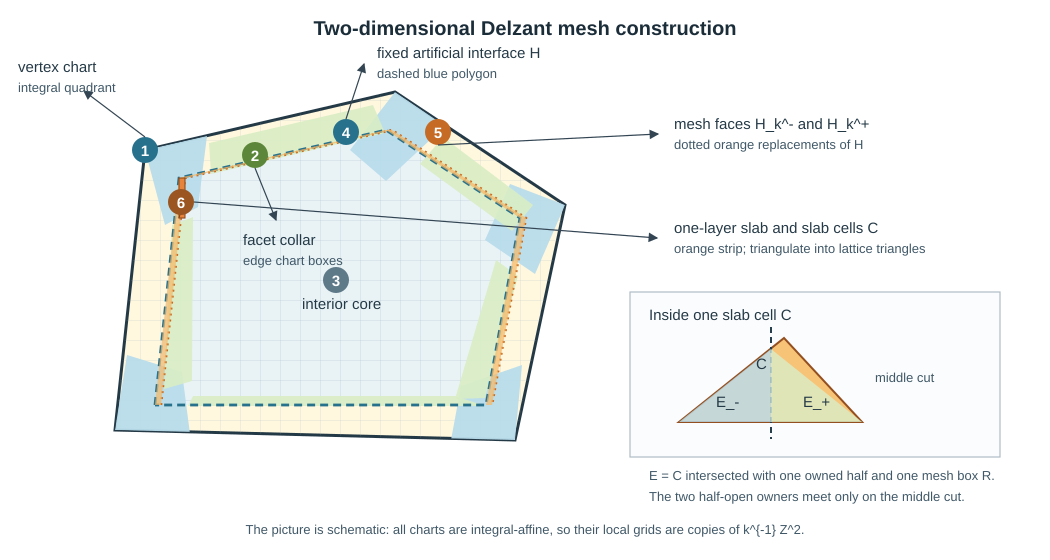
\includegraphics[width=.92\textwidth]{delzant_mesh_2d_construction.pdf}
\\[-2mm]
{\small\itshape Two-dimensional Delzant mesh construction.}
\end{center}

First fix a vertex $p$. If $F_1,F_2$ are the two incident edges, the
Delzant condition says that $(l_{F_1},l_{F_2})$ is an integral-affine
chart near $p$: it maps the ambient lattice to $\mathbb Z^2$, preserves
area, and writes $P$ locally as the quadrant $x_1,x_2\geq0$. Choose a
small coordinate rectangle in this quadrant and call it a \emph{vertex
chart}; this is region $1$ in the figure. Do this at every vertex,
choosing the rectangles disjoint after the usual half-open convention.
The convention assigns a common grid edge to just one neighboring
rectangle, and is used only to prevent double counting.

Second, after removing the vertex rectangles, the remaining part of
each edge $F$ is a compact interval in $\operatorname{relint}F$.
Choose an integral-affine \emph{edge chart} $(l_F,y)$ there, where
$l_F$ is the primitive inward normal coordinate and $y$ is an integral
tangential coordinate. A product $[0,\delta]\times I$ in these
coordinates is the \emph{facet collar}; it is region $2$. On its
overlap with a vertex chart, retain the already chosen normal coordinate
and subdivide only in the tangential direction. Hence the two box
decompositions agree on their overlap, rather than creating an
interface there. The collar is chosen wide enough that each prescribed
$K_F$ lies in its edge boxes and avoids all later cuts.

Third, remove the vertex charts and all facet collars. The closure of
what remains is the compact \emph{interior core}, region $3$, and is
given one fixed integral-affine box chart. The inner boundary of a
collar and any remaining chart-change boundary are fixed rational
segments in $\operatorname{int}P$; each such segment is an
\emph{artificial interface} $H$, shown by the blue dashed line in
region $4$. It is artificial because it is neither an edge of $P$ nor
a prescribed part of the quadrature formula. The finitely many $H$'s
are chosen in general position, so two distinct ones meet, if at all,
in finitely many points.

Fourth, only now fix $k$. Subdivide each chart by its coordinate lines
$x_i=j/k$. The two box meshes adjacent to $H$ usually do not share a
common mesh edge. Extend each mesh one layer across $H$ and replace $H$
from its two sides by the nearest unions of mesh faces, denoted
$H_k^-$ and $H_k^+$ in region $5$. Their separation is $O(k^{-1})$;
the closed region between them is the \emph{one-layer slab}. If two
interfaces meet, first enlarge their $O(k^{-1})$ overlap by the mesh
cells meeting it, and call the resulting cells junction cells.

Finally, triangulate each slab polytope using its lattice vertices.
In dimension two a \emph{slab cell} $C$ is therefore a lattice triangle
with three vertices, as in region $6$. For the actual convex
quadrature on $C$, use its barycentric coordinates, producing the
coefficients $\beta_{C,u}$. For the reference coefficients, divide the
slab by a middle segment between the two extended meshes. Its two
half-open sides are \emph{owned} by the left and right charts: the
middle segment itself is assigned by a fixed convention and has zero
area. Intersect a triangle $C$ with one owned side and then with one
mesh box $R$ of its owner. Every nonempty set
\[
E=C\cap\{\text{owned half of the slab}\}\cap R
\]
is an \emph{owned piece}. It need not be a triangle. The multilinear
box coordinates $\lambda_{R,u}$ give
\[
q_{E,u}=k^2\int_E\lambda_{R,u}\,\mathrm dx,
\qquad
\bar\beta_{C,u}=\sum_{E\subset C}q_{E,u}.
\]
Thus $\beta_{C,\bullet}$ controls the integral by convexity, whereas
$\bar\beta_{C,\bullet}$ is charged to ordinary box-corner incidences.
Their equal total mass makes $\beta_{C,\bullet}-\bar\beta_{C,\bullet}$
annihilate constants; this is the source of the modulus-of-continuity
error at an ordinary interface cell.
\end{rem}

\begin{lem}[convex $L^2$ compactness]
\label{lem: convex L2 compactness}
Let $P$ be a full-dimensional lattice polytope. If
$f_k\in\mathcal C(P)$ and $\sup_k\|f_k\|_{k,2}<\infty$, then, after
passing to a subsequence, there is a convex $f\in L^2(P)$ such that
$f_k\rightharpoonup f$ weakly in $L^2(P)$ and $f_k\to f$ locally
uniformly on $\operatorname{int}P$.
\end{lem}

\begin{proof}
By (\ref{eq: detailed discrete continuous bound}), the sequence
$\{f_{k}\}$ is bounded in $L^{2}(P)$, so a subsequence converges
weakly to some $f\in L^{2}(P)$. Convexity passes to the weak limit:
for every nonnegative $\chi\in C_{c}^{\infty}(\mathrm{int}P)$ and
every vector $\xi$,
\[
\int_{P}f_{k}\,\partial_{\xi\xi}\chi\,\mathrm{d}x\geq0.
\]
Weak convergence permits passage to the limit. Thus the
distributional Hessian of $f$ is nonnegative, and the standard
distributional characterization of convexity gives a convex
representative of $f$, which we continue to denote by $f$.

For each $K\Subset K'\Subset\mathrm{int}P$, Lemma
\ref{lem: interior C0 estimate}, together with
$\|f_k\|_{L^1(K')}\leq |K'|^{1/2}\|f_k\|_{L^2(P)}$, gives a uniform
$C^0$ bound on $K$. Lemma \ref{lem: interior Lipschitz estimate} gives,
separately, a uniform Lipschitz bound there. Hence $\{f_k\}$ is
uniformly bounded and equicontinuous on $K$. Choose
an exhaustion
$K_{1}\Subset K_{2}\Subset\cdots\Subset\mathrm{int}P$.
Arzelà--Ascoli first gives a uniformly convergent subsequence on
$K_{1}$; from it choose one converging on $K_{2}$, and continue
inductively. The diagonal subsequence converges locally uniformly on
$\mathrm{int}P$. Local uniform convergence implies distributional
convergence, while the same subsequence converges weakly in $L^{2}$;
therefore its local uniform limit is the weak limit $f$.
\end{proof}

\begin{lem}[Delzant boundary liminf]
\label{lem: Delzant boundary liminf}
Assume that $P$ is Delzant. Let $f_k\in\mathcal C(P)$ be bounded in
$\|\cdot\|_{k,2}$ and suppose that $f_k\rightharpoonup f$ in $L^2(P)$
and locally uniformly on $\operatorname{int}P$. With the lower
semicontinuous extension of $f$ to $P$, one has
\begin{equation}
\liminf_{k\to\infty}B_k(f_k)\geq
\int_{\partial P}f\,\mathrm d\sigma,
\label{eq: detailed boundary liminf}
\end{equation}
where the right-hand side is allowed to be $+\infty$.
\end{lem}

\begin{proof}
Fix compact polytopes $K_{F}\Subset\operatorname{relint}F$, one for
each facet. Applying (\ref{eq: lattice trapezoid estimate}) to a
nonnegative convex sequence $g_{k}$ and recalling the definition of
$B_{k}$ gives the explicit estimate
\begin{equation}
B_{k}(g_{k})\geq
\sum_{F}\frac{1}{k^{n-1}}
\sum_{y\in K_{F}\cap P_{k}}g_{k}(y)
-\frac{C}{k}\sup_Qg_k-C\omega_{g_k,Q}(C/k).
\label{eq: facet lattice lower bound}
\end{equation}
The coefficient is $1$ because the facet weight $1/2$ in
(\ref{eq: lattice trapezoid estimate}) is multiplied by the factor
$2$ in $B_{k}$. The first error tends to zero by the interior $C^0$
estimate. For the second, first use the modulus itself and then use
$\omega_{g_k,Q}(C/k)\leq Ck^{-1}\operatorname{Lip}_Q(g_k)$ together
with the separate interior Lipschitz estimate.

Apply this estimate to $g_k=f_k-\ell_k$ below. Fix a point
$p\in\mathrm{int}P$ and choose
$q_{k}\in\partial f_{k}(p)$. Local uniform boundedness on a ball
around $p$ implies that $\{q_{k}\}$ is bounded: if
$B(p,2r)\Subset P$, the subgradient inequality at
$p\pm r e_{i}$ gives
\[
|\langle q_{k},e_{i}\rangle|
\leq r^{-1}\left(
|f_{k}(p+r e_{i})|+|f_{k}(p-r e_{i})|+2|f_{k}(p)|\right).
\]
After passing to a further subsequence, the supporting affine
functions
\[
\ell_{k}(x)=f_{k}(p)+\langle q_{k},x-p\rangle
\]
converge uniformly to an affine function $\ell$, and
$g_{k}=f_{k}-\ell_{k}\geq0$ converges locally uniformly to
$g=f-\ell$ on $\mathrm{int}P$.

For every facet $F$, primitivity of $l_{F}$ gives an integral vector
$v_{F}$ with $l_{F}(v_{F})=1$. Since $K_{F}$ is separated from all
the other facets, this vector points into $P$ above $K_{F}$ for a
sufficiently short time. Thus we may choose $\delta>0$ so small that
\[
\{y+t v_{F}\mid y\in K_{F},\ 0\leq t\leq2\delta\}
\Subset P\setminus\bigcup_{F'\neq F}F'.
\]
Put $m_{k}=\lfloor k\delta\rfloor$. Then
$y+jv_{F}/k\in P_{k}$ for $y\in K_{F}\cap P_{k}$ and
$0\leq j\leq2m_{k}$, once $k$ is sufficiently large.

For $y\in K_{F}\cap k^{-1}\mathbb{Z}^{n}$, convexity on the segment
$[y,y+2m_{k}v_{F}/k]$ gives
\begin{equation}
g_{k}(y)\geq
2g_{k}(y+m_{k}v_{F}/k)-g_{k}(y+2m_{k}v_{F}/k).
\label{eq: recover boundary value}
\end{equation}
Both points on the right stay in a compact subset of
$\mathrm{int}P$. Hence local uniform convergence and the ordinary
Riemann-sum theorem on $F$ imply, using
(\ref{eq: facet lattice lower bound}), the uniform interior $C^0$
bound, and the uniform interior Lipschitz bound,
\[
\liminf_{k\rightarrow\infty}B_{k}(g_{k})
\geq\sum_{F}\int_{K_{F}}
\left(2g(y+\delta v_{F})-g(y+2\delta v_{F})\right)
\,\mathrm{d}\sigma_{F}.
\]
For a one-dimensional convex function $t\mapsto g(y+t v_{F})$, the
quantities
$2g(y+\delta v_{F})-g(y+2\delta v_{F})$ converge increasingly along
dyadic $\delta\downarrow0$ to the lower semicontinuous boundary value
$g(y)$. Indeed, if $\phi(t)=g(y+t v_{F})$, monotonicity of the secant
slopes gives
\[
2\bigl(\phi(t)-\phi(t/2)\bigr)
\leq\phi(2t)-\phi(t),
\]
which is exactly
$2\phi(t/2)-\phi(t)\geq2\phi(t)-\phi(2t)$. The limit is
$\phi(0)$ by the definition of the lower semicontinuous extension.
On a fixed $K_{F}$ these functions have a common lower bound after
restricting to $0<\delta\leq\delta_{0}$, because their possible
negative part is bounded by $g(y+2\delta v_{F})$ on a compact subset
of the interior. We may therefore add one constant and apply monotone
convergence. We first let dyadic $\delta\downarrow0$ and then take an
increasing exhaustion $K_{F}\nearrow\mathrm{relint}F$. A second
application of monotone convergence gives
\[
\liminf_{k\rightarrow\infty}B_{k}(g_{k})
\geq\sum_{F}\int_{F}g\,\mathrm{d}\sigma_{F}.
\]
Finally, the affine Ehrhart formula and
$\ell_{k}\to\ell$ uniformly give
$B_{k}(\ell_{k})\to\int_{\partial P}\ell\,\mathrm{d}\sigma$.
Since $f_{k}=g_{k}+\ell_{k}$, we obtain
\begin{equation}
\liminf_{k\rightarrow\infty}B_{k}(f_{k})
\geq\int_{\partial P}f\,\mathrm{d}\sigma.
\end{equation}
If the right-hand side is $+\infty$, the same argument applied to an
increasing exhaustion by the $K_{F}$ shows that the left-hand side
is $+\infty$ as well.
\end{proof}

\begin{lem}[quadratic liminf]
\label{lem: quadratic liminf}
Let $P$ be a full-dimensional lattice polytope. Under the convergence
conclusion of Lemma \ref{lem: convex L2 compactness},
\begin{equation}
\liminf_{k\to\infty}\|f_k\|_{k,2}^2\geq\|f\|_{L^2(P)}^2.
\label{eq: quadratic liminf}
\end{equation}
\end{lem}

\begin{proof}
Write $P^\delta=\{x\in P:l_F(x)\geq\delta\text{ for every facet }F\}$.
Fix $\delta>0$ for which $P^{\delta}$ has nonempty interior. Local
uniform convergence and the ordinary Riemann-sum theorem give
\[
\lim_{k\rightarrow\infty}\frac{1}{k^{n}}
\sum_{u\in P_{k}\cap P^{\delta}}f_{k}(u)^{2}
=\int_{P^{\delta}}f^{2}\,\mathrm{d}x.
\]
All omitted summands are nonnegative, hence
\[
\liminf_{k\rightarrow\infty}\left\Vert f_{k}\right\Vert _{k,2}^{2}
\geq\int_{P^{\delta}}f^{2}\,\mathrm{d}x.
\]
Letting $\delta\downarrow0$ and using monotone convergence proves
\[
\liminf_{k\rightarrow\infty}\left\Vert f_{k}\right\Vert _{k,2}^{2}
\geq\left\Vert f\right\Vert _{L^{2}(P)}^{2}.
\]
\end{proof}

\begin{lem}[no discrete $L^2$ defect]
\label{lem: no discrete L2 defect}
Under the hypotheses of Lemma \ref{lem: quadratic liminf}, assume in
addition that
\begin{equation}
\lim_{k\to\infty}\|f_k\|_{k,2}^2=\|f\|_{L^2(P)}^2.
\label{eq: no discrete L2 defect}
\end{equation}
Then $f_k\to f$ strongly in $L^2(P)$.
\end{lem}

\begin{proof}
Assume now (\ref{eq: no discrete L2 defect}).
For every fixed $\delta>0$, the interior Riemann-sum convergence then
implies
\begin{align}
\limsup_{k\rightarrow\infty}\frac{1}{k^{n}}
\sum_{u\in P_{k}\setminus P^{\delta}}f_{k}(u)^{2}
&\leq\left\Vert f\right\Vert _{L^{2}(P)}^{2}
-\int_{P^{\delta}}f^{2}\,\mathrm{d}x\nonumber\\
&=\int_{P\setminus P^{\delta}}f^{2}\,\mathrm{d}x.
\label{eq: boundary discrete mass}
\end{align}
For each $k$, apply (\ref{eq: supporting affine control}) to $f_k$
and write
\[
f_k=g_k+\ell_k,\qquad g_k\geq0,
\qquad \|\ell_k\|_{C^0(P)}\leq C\|f_k\|_{k,2}\leq C.
\]
Set $E=P\setminus P^{2\delta}$ and
\[
U_{k,\delta}=\{u\in P_k:\operatorname{dist}(u,E)\leq C/k\}.
\]
For all sufficiently large $k$, one has
$U_{k,\delta}\subset P_k\setminus P^\delta$. Moreover, the boundary
strip $E$ has volume at most $C\delta$, and
$|U_{k,\delta}|\leq C(k^n\delta+k^{n-1})$. Using
(\ref{eq: local nonnegative sampling estimate}) for $g_k$, followed
by $g_k^2\leq2f_k^2+2\ell_k^2$, gives
\begin{align*}
\int_E f_k^2\,\mathrm{d}x
&\leq2\int_E g_k^2\,\mathrm{d}x
+2|E|\|\ell_k\|_{C^0(P)}^2\\
&\leq\frac{C}{k^n}\sum_{u\in U_{k,\delta}}f_k(u)^2
+C\left(k^{-n}|U_{k,\delta}|+|E|\right)
\|\ell_k\|_{C^0(P)}^2.
\end{align*}
For fixed $\delta$, the last coefficient is at most $C\delta$ once
$k$ is sufficiently large. Hence (\ref{eq: boundary discrete mass})
implies
\[
\limsup_{k\rightarrow\infty}
\int_{P\setminus P^{2\delta}}f_{k}^{2}\,\mathrm{d}x
\leq C\int_{P\setminus P^{\delta}}f^{2}\,\mathrm{d}x+C\delta.
\]
On $P^{2\delta}$ the convergence is uniform, hence strong in
$L^{2}$. Therefore
\begin{align*}
\limsup_{k\rightarrow\infty}
\left\Vert f_{k}-f\right\Vert _{L^{2}(P)}^{2}
&\leq2\limsup_{k\rightarrow\infty}
\int_{P\setminus P^{2\delta}}f_{k}^{2}\,\mathrm{d}x
+2\int_{P\setminus P^{2\delta}}f^{2}\,\mathrm{d}x\\
&\leq2C\int_{P\setminus P^{\delta}}f^{2}\,\mathrm{d}x+2C\delta
+2\int_{P\setminus P^{2\delta}}f^{2}\,\mathrm{d}x.
\end{align*}
All terms tend to zero as $\delta\downarrow0$, because
$f\in L^{2}(P)$. Hence $f_{k}\to f$ strongly in $L^{2}(P)$, which
proves the last assertion.
\end{proof}

\begin{rem}
The Delzant hypothesis in Lemma
\ref{lem: Delzant boundary liminf} cannot be omitted for a general
lattice polytope. For example, let
\[
P_{m}=\operatorname{conv}\{(0,0),(1,0),(1,m)\},\qquad m>6,
\]
and write a point as $(x_{1},x_{2})$. The primitive edge directions
at the origin have determinant $m$, so $P_{m}$ is not Delzant. The
convex functions
\[
g_{k}(x_{1},x_{2})=k\max\{1-kx_{1},0\}
\]
vanish at every point of $(P_{m})_{k}$ except the origin, where their
value is $k$. Therefore
\[
\Vert g_{k}\Vert_{k,2}^{2}=1,
\qquad
\int_{P_{m}}g_{k}\,\mathrm{d}x
=\int_{0}^{1/k}kmx_{1}(1-kx_{1})\,\mathrm{d}x_{1}
=\frac{m}{6k},
\]
and hence
\[
B_{k}(g_{k})=\frac{2}{k}
\left(k-k^{2}\frac{m}{6k}\right)
=2\left(1-\frac{m}{6}\right)<0.
\]
On the other hand, $g_{k}\to0$ locally uniformly away from the origin
and $g_{k}\rightharpoonup0$ weakly in $L^{2}(P_{m})$; indeed
$\int_{P_{m}}g_{k}^{2}\,\mathrm{d}x=m/12$. Thus the boundary liminf
in (\ref{eq: detailed boundary liminf}) would read
$2(1-m/6)\geq0$, which is false. The lattice-box weights in
(\ref{eq: box trapezoid}) explain exactly why smoothness of the
transverse lattice cones removes this defect.
\end{rem}

\begin{proof}[Proof of Theorem \ref{thm:main converge}]
\label{proof of convergence} Put $\psi=-\Theta_{P}$. By Proposition
\ref{prop: recharac Theta} and Theorem \ref{thm: theta is continuous-INTRO},
$\psi\in\mathcal{C}(P)$ is the unique minimizer of $\Psi$. Minimality
of $\psi_{k}$ and (\ref{eq:EM}) give
\begin{equation}
\limsup_{k\rightarrow\infty}\Psi_{k}(\psi_{k})
\leq\lim_{k\rightarrow\infty}\Psi_{k}(\psi)
=\Psi(\psi)=\inf\Psi.\label{eq: minimizer limsup}
\end{equation}
On the other hand, (\ref{eq: convex quadrature coercivity}) and Young's
inequality imply
\[
\Psi_{k}(f)\geq\frac{1}{2}\left\Vert f\right\Vert _{k,2}^{2}
-C_{P}\left\Vert f\right\Vert _{k,2}
\geq\frac{1}{4}\left\Vert f\right\Vert _{k,2}^{2}-C_{P}^{2}.
\]
Together with (\ref{eq: minimizer limsup}), this shows that
$\sup_{k}\left\Vert\psi_{k}\right\Vert _{k,2}<\infty$.

\textbf{Step 1}. We first prove convergence of the discrete quadratic
terms. Set
\[
a_{k}\coloneqq\left\Vert\psi_{k}\right\Vert _{k,2}^{2}.
\]
The preceding coercivity argument shows that $\{a_{k}\}$ is bounded.
Let $A$ be any subsequential limit of $\{a_{k}\}$, and choose a
subsequence $\{k_{j}\}$ such that
\begin{equation}
\lim_{j\rightarrow\infty}a_{k_{j}}=A.\label{eq: choose discrete norm limit}
\end{equation}
Lemma \ref{lem: convex L2 compactness}, applied to
$\{\psi_{k_{j}}\}$, provides a further subsequence, still denoted by
$\{k_{j}\}$, and a convex function $u\in L^{2}(P)$ such that
\[
\psi_{k_{j}}\rightharpoonup u\quad\text{weakly in }L^{2}(P),\qquad
\psi_{k_{j}}\longrightarrow u\quad\text{locally uniformly on }
\mathrm{int}P.
\]
We claim first that $\int_{\partial P}u\,\mathrm{d}\sigma$ is finite.
Indeed, if it were $+\infty$, then
(\ref{eq: choose discrete norm limit}) and
(\ref{eq: detailed boundary liminf}) would imply
\[
\liminf_{j\rightarrow\infty}\Psi_{k_{j}}(\psi_{k_{j}})
\geq\frac{1}{2}A+\int_{\partial P}u\,\mathrm{d}\sigma=+\infty,
\]
contradicting (\ref{eq: minimizer limsup}). Thus
$u\in\mathcal{C}_{1}(P)\cap L^{2}(P)$ and $\Psi(u)$ is well-defined.

Since $a_{k_{j}}\rightarrow A$, the elementary inequality
$\liminf(x_{j}+y_{j})\geq\lim x_{j}+\liminf y_{j}$ and
(\ref{eq: detailed boundary liminf}) and
(\ref{eq: quadratic liminf}) give
\begin{align*}
\liminf_{j\rightarrow\infty}\Psi_{k_{j}}(\psi_{k_{j}})
&=\liminf_{j\rightarrow\infty}
\left(\frac{1}{2}a_{k_{j}}+B_{k_{j}}(\psi_{k_{j}})\right)\\
&\geq\frac{1}{2}A+\liminf_{j\rightarrow\infty}
B_{k_{j}}(\psi_{k_{j}})\\
&\geq\frac{1}{2}A+\int_{\partial P}u\,\mathrm{d}\sigma\\
&\geq\frac{1}{2}\left\Vert u\right\Vert _{L^{2}(P)}^{2}
+\int_{\partial P}u\,\mathrm{d}\sigma
=\Psi(u).
\end{align*}
Here the last inequality uses
$A=\lim_{j}a_{k_{j}}\geq\left\Vert u\right\Vert _{L^{2}(P)}^{2}$,
which is Lemma \ref{lem: quadratic liminf}.
Combining this with (\ref{eq: minimizer limsup}) and the minimality of
$\psi$ gives the complete chain
\begin{align*}
\Psi(\psi)
&\geq\limsup_{j\rightarrow\infty}\Psi_{k_{j}}(\psi_{k_{j}})
\geq\liminf_{j\rightarrow\infty}\Psi_{k_{j}}(\psi_{k_{j}})\\
&\geq\frac{1}{2}A+\int_{\partial P}u\,\mathrm{d}\sigma
\geq\Psi(u)\geq\Psi(\psi).
\end{align*}
Hence every inequality in this chain is an equality. In particular,
$\Psi(u)=\Psi(\psi)$, so the uniqueness of the minimizer of $\Psi$
implies
\begin{equation}
u=\psi.\label{eq: weak limit is psi}
\end{equation}
Moreover, the equality chain contains the identity
\[
\frac{1}{2}A+\int_{\partial P}u\,\mathrm{d}\sigma
=\Psi(u)
=\frac{1}{2}\left\Vert u\right\Vert _{L^{2}(P)}^{2}
+\int_{\partial P}u\,\mathrm{d}\sigma.
\]
Since the boundary integral is finite, subtracting it from both sides
gives
\[
A=\left\Vert u\right\Vert _{L^{2}(P)}^{2}
=\left\Vert\psi\right\Vert _{L^{2}(P)}^{2}.
\]
Thus every subsequential limit of the bounded sequence $\{a_{k}\}$
equals $\left\Vert\psi\right\Vert _{L^{2}(P)}^{2}$. It follows that
the whole sequence converges:
\begin{equation}
\lim_{k\rightarrow\infty}\left\Vert\psi_{k}\right\Vert _{k,2}^{2}
=\left\Vert\psi\right\Vert _{L^{2}(P)}^{2}.
\label{eq: full discrete norm convergence}
\end{equation}
For completeness, if this conclusion failed, there would be an
$\varepsilon>0$ and a subsequence along which
$|a_{k}-\left\Vert\psi\right\Vert _{L^{2}(P)}^{2}|\geq\varepsilon$.
Boundedness would give a further convergent subsequence, whose limit
would be a subsequential limit different from
$\left\Vert\psi\right\Vert _{L^{2}(P)}^{2}$, a contradiction.

\textbf{Step 2}. We next prove strong $L^{2}$ convergence of the
functions. Let $\{\psi_{k_{j}}\}$ be an arbitrary subsequence. By
Lemma \ref{lem: convex L2 compactness}, after passing to a
further subsequence $\{\psi_{k_{j_{\ell}}}\}$, there is a convex
$v\in L^{2}(P)$ such that
\[
\psi_{k_{j_{\ell}}}\rightharpoonup v\quad\text{weakly in }L^{2}(P)
\]
and the convergence is locally uniform on $\mathrm{int}P$. The
boundary integral of $v$ must be finite: otherwise the boundary
liminf in (\ref{eq: detailed boundary liminf}) would contradict
(\ref{eq: minimizer limsup}), exactly as in Step 1. Hence
$v\in\mathcal{C}_{1}(P)\cap L^{2}(P)$.

By (\ref{eq: full discrete norm convergence}),
\[
\lim_{\ell\rightarrow\infty}
\left\Vert\psi_{k_{j_{\ell}}}\right\Vert _{k_{j_{\ell}},2}^{2}
=\left\Vert\psi\right\Vert _{L^{2}(P)}^{2}.
\]
Lemma \ref{lem: quadratic liminf} first
shows that
$\left\Vert\psi\right\Vert _{L^{2}(P)}^{2}
\geq\left\Vert v\right\Vert _{L^{2}(P)}^{2}$. Using this inequality,
the boundary liminf, (\ref{eq: minimizer limsup}), and minimality of
$\psi$, we obtain
\begin{align*}
\Psi(\psi)
&\geq\liminf_{\ell\rightarrow\infty}
\Psi_{k_{j_{\ell}}}(\psi_{k_{j_{\ell}}})\\
&\geq\frac{1}{2}\left\Vert\psi\right\Vert _{L^{2}(P)}^{2}
+\int_{\partial P}v\,\mathrm{d}\sigma\\
&\geq\frac{1}{2}\left\Vert v\right\Vert _{L^{2}(P)}^{2}
+\int_{\partial P}v\,\mathrm{d}\sigma
=\Psi(v)\geq\Psi(\psi).
\end{align*}
Thus equality holds throughout. The uniqueness of the minimizer gives
$v=\psi$, and consequently
\[
\lim_{\ell\rightarrow\infty}
\left\Vert\psi_{k_{j_{\ell}}}\right\Vert _{k_{j_{\ell}},2}^{2}
=\left\Vert v\right\Vert _{L^{2}(P)}^{2}.
\]
Therefore the hypothesis of Lemma \ref{lem: no discrete L2 defect}
is satisfied. That lemma yields
\[
\psi_{k_{j_{\ell}}}\longrightarrow\psi
\quad\text{strongly in }L^{2}(P).
\]
We have proved that every subsequence of $\{\psi_{k}\}$ has a further
subsequence converging strongly to $\psi$. This implies convergence
of the whole sequence. Indeed, otherwise there would be an
$\varepsilon>0$ and a subsequence $\{\psi_{k_{j}}\}$ satisfying
\[
\left\Vert\psi_{k_{j}}-\psi\right\Vert _{L^{2}(P)}\geq\varepsilon
\quad\text{for every }j,
\]
but this subsequence would have a further subsequence converging
strongly to $\psi$, which is impossible. Hence
\begin{equation}
\psi_{k}\longrightarrow\psi=-\Theta_{P}
\quad\text{strongly in }L^{2}(P).\label{eq: strong L2 psi}
\end{equation}
Since $\psi=-\Theta_{P}$, (\ref{eq: full discrete norm convergence})
is precisely (\ref{eq: discrete L2 converge}). Furthermore,
(\ref{eq: quantum mini}) and (\ref{eq: strong L2 psi}) give
\[
\left\Vert V_{P}k^{n}\sigma_{k}^{\vee}-1
+\frac{\Theta_{P}}{2k}\right\Vert _{L^{2}(P)}
=\frac{1}{2k}\left\Vert\psi_{k}+\Theta_{P}\right\Vert _{L^{2}(P)}
=\mathrm{o}(k^{-1}),
\]
which proves (\ref{eq: dream converge L2}).

\textbf{Step 3}. Finally, assume that $\{\psi_{k}\}$ is
$C^{0}$-precompact. We show that the convergence is uniform. If not,
there would be an $\varepsilon>0$ and a subsequence $\{\psi_{k_{j}}\}$
such that
\begin{equation}
\left\Vert\psi_{k_{j}}-\psi\right\Vert _{C^{0}(P)}
\geq\varepsilon\quad\text{for every }j.\label{eq: not uniform}
\end{equation}
By $C^{0}$-precompactness, a further subsequence converges uniformly
to some $w\in\mathcal{C}(P)$. Uniform convergence implies convergence
to $w$ in $L^{2}(P)$, whereas (\ref{eq: strong L2 psi}) says that the
same subsequence converges to $\psi$ in $L^{2}(P)$. Uniqueness of the
$L^{2}$ limit gives $w=\psi$ almost everywhere. Both functions are
continuous on $P$, so $w=\psi$ everywhere. The further subsequence
therefore converges uniformly to $\psi$, contradicting
(\ref{eq: not uniform}). Thus $\psi_{k}\rightarrow\psi$ uniformly.
Finally,
\[
\left\Vert V_{P}k^{n}\sigma_{k}^{\vee}-1
+\frac{\Theta_{P}}{2k}\right\Vert _{C^{0}(P)}
=\frac{1}{2k}\left\Vert\psi_{k}+\Theta_{P}\right\Vert _{C^{0}(P)}
=\mathrm{o}(k^{-1}),
\]
which is (\ref{eq: dream converge}).
\end{proof}

\begin{rem}
The theorem gives unconditional $L^{2}$ convergence but does not control
values on lower-dimensional faces. To obtain uniform convergence, we
still need to verify the $C^{0}$-precompactness of
$\psi_{k}=2V_{P}k^{n+1}\sigma^{\vee}_{k}-2k$.

Here is why the preceding $L^{2}$ and convexity estimates do not by
themselves remove this hypothesis. Take the Delzant square
$P=[0,1]^{2}$ and define
\[
h_{k}(x,y)=\max\{1-k(x+y),0\}.
\]
This is convex, $h_k(0,0)=1$, and $h_k$ vanishes at every point of
$P_k$ other than $(0,0)$. Consequently,
\[
\|h_k\|_{k,2}^{2}=k^{-2},\qquad
\|h_k\|_{L^{2}(P)}^{2}
=\int_{0}^{1/k}s(1-ks)^{2}\,\mathrm{d}s=\frac{1}{12k^{2}},
\qquad \|h_k\|_{C^{0}(P)}=1.
\]
Thus even strong $L^{2}$ convergence and local uniform convergence on
$\operatorname{int}P$ do not imply uniform convergence for convex
functions on a Delzant polytope. This example does not concern the
special minimizers $\psi_k$; it shows that a proof for $\psi_k$ must
use additional information on the shortest GKZ vectors, for example
a quantitative estimate controlling the coordinates of $\sigma_k$ on
vertices and, more generally, on lower-dimensional faces. Such an
estimate is not a consequence of the $L^2$ compactness and quadrature
lemmas above.
\end{rem}


\section*{Remaining questions\label{sec:Remaining-questions}}
\begin{enumerate}
\item Show the sequence $\psi_{k}$ is uniformly bounded and equicontinuous,
thereby upgrading the unconditional $L^{2}$ convergence in Theorem
\ref{thm:main converge} to uniform convergence.
\item Since Theorem \ref{thm: Gabor paper} (4) shows that $\Theta_{P}$
induces a semistable decomposition of $P$, we should investigate
the semistability of each piece of the subdivision induced by $\sigma_{A}$. 
\item Is there a relation between the asymptotics of $\Sigma(P_{k})$ and
the space $\mathcal{S}(P)$ (\ref{eq: space of scalar curvature})
of prescribed scalar curvatures?
\item An effective algorithm to compute $\sigma_{A}$ without knowing the
entire secondary polytope. 
\end{enumerate}
\appendix

\section{\label{appendix} Two-terms expansion for Riemann sum of convex functions}

We establish a folklore expansion of Riemann sum, which is crucial
in the proof of Theorem \ref{thm:main converge}.
\begin{thm}
Let $P\subset\mathbb{R}^{n}$ be a full-dimensional lattice polytope.
For any $k\in\mathbb{Z}_{>0}$,
set $P_{k}=P\cap k^{-1}\mathbb{Z}^{n}$. Let $f_{k}:P\rightarrow\mathbb{R}$
be a sequence of convex functions (continuous up to $\partial P$)
which uniformly converges to $f$. Then we have
\begin{equation}
\lim_{k\rightarrow\infty}\frac{1}{k^{n-1}}\left(\sum_{u\in P_{k}}f_{k}(u)-k^{n}\int_{P}f_{k}\ \mathrm{d}x\right)=\frac{1}{2}\int_{\partial P}f\ \mathrm{d}\sigma.\label{eq:EM enhanced}
\end{equation}
In particular, when $f_{k}=f$ for all $k$, we have expansion
\begin{equation}
\sum_{u\in P_{k}}f(u)=k^{n}\int_{P}f\ \mathrm{d}x+\frac{k^{n-1}}{2}\int_{\partial P}f\ \mathrm{d}\sigma+\mathrm{o}(k^{n-1}).\label{eq:EM}
\end{equation}
In the above, $\mathrm{d}x$ is the standard Lebesgue measure, and
the boundary measure $\mathrm{d}\sigma$ is defined as follows. For
each facet $F\subset\partial P$, choose $p_F\in F\cap\mathbb Z^n$
and set $\Lambda_F=(\mathrm{Aff}(F)-p_F)\cap\mathbb Z^n$.
Then $\mathrm{d}\sigma|_{F}$ is the translation-invariant measure
on $\mathrm{Aff}(F)$ for which the lattice $\Lambda_F$ has covolume
one. This definition is independent of the choice of $p_F$.
\end{thm}

\begin{rem}
(1) when $f$ is smooth on an open set containing $P$, (\ref{eq:EM})
is just the leading two terms of the Euler--Maclaurin expansion.
This expansion holds for every lattice polytope; no simplicity or
unimodularity assumption, and hence no Delzant assumption, is needed. See
\cite{tate_asymptotic_2011} and its references. (2) if $f$ is merely continuous, (\ref{eq:EM})
may fail even in one dimension (Weierstrass type functions). (3) If
$f$ is convex and piece-wisely linear with rational coefficients,
(\ref{eq:EM}) can be derived from the asymptotics of lattice point
counting, see \cite[Prop. 4.1.3]{donaldson_scalar_2002}. In our setting,
(\ref{eq:EM}) cannot be derived from these results via a direct approximation.
The key in the following proof is decomposing the Riemann sum into
interior part and boundary part, and we handle the boundary part via
approximation.
\end{rem}

\begin{proof}
\textbf{Step 1}. We extend $f_{k},f$ to $\mathbb{R}^{n}$ such that
uniform convergence still holds and they share a common continuity
modulus $\hat{\omega}$, i.e. for $g=f_{k}$ or $f$, we have
\[
\left|g(x_{1})-g(x_{2})\right|\leq\hat{\omega}\left(\left\Vert x_{1}-x_{2}\right\Vert \right),\ \forall x_{i}\in\mathbb{R}^{n}.
\]
We will use the norm $\left\Vert x\right\Vert =\max_{1\leq i\leq n}\left|x_{i}\right|$
and distance $d(x,y)=\left\Vert x-y\right\Vert $. Let
\[
\omega_{k}(\delta)\coloneqq\sup\left\{ \left|f_{k}(x)-f_{k}(y)\right|\mid x,y\in P,\ d(x,y)\leq\delta\right\} ,
\]
be the minimal continuity modulus of $f_{k}$. By uniform convergence,
the family $\{f_k\}$ is equicontinuous on the compact set $P$.
Indeed, the tail of the sequence is uniformly close to the continuous
function $f$, while a finite initial part has a common continuity
modulus. Consequently,
\[
\omega(\delta)\coloneqq\sup_{k}\omega_{k}(\delta)\rightarrow0,\text{ as }\delta\rightarrow0.
\]
The same estimate holds for the uniform limit $f$. Thus, for
$g=f_{k}$ or $f$, we have
\[
\left|g(x)-g(y)\right|\leq\omega\left(\left\Vert x-y\right\Vert \right),\ \forall x,y\in P.
\]
To apply McShane's extension, take a nondecreasing concave majorant
$\hat{\omega}$ of $\omega$, with $\hat{\omega}(0)=0$ and
$\hat{\omega}(\delta)\rightarrow0$ as $\delta\rightarrow0$.
Such a concave modulus exists for every common modulus of continuity.
It is subadditive, i.e.
$\hat{\omega}(\delta_{1}+\delta_{2})\leq\hat{\omega}(\delta_{1})+\hat{\omega}(\delta_{2})$.
Then we define McShane's extension:
\[
\tilde{f}_{k}(x)\coloneqq\inf_{y\in P}f_{k}(y)+\hat{\omega}\left(\left\Vert x-y\right\Vert \right),\ \forall x\in\mathbb{R}^{n},
\]
and $\tilde{f}(x)$ is defined similarly. For $x\in P$, the choice
$y=x$ gives $\tilde f_k(x)\leq f_k(x)$, whereas the modulus estimate
on $P$ gives the reverse inequality. Thus the extension coincides
with the original function on $P$.

They share a common continuity modulus $\hat{\omega}$. For any $x_{1},x_{2}\in\mathbb{R}^{n}$
and $y\in P$, by the subadditivity, we have
\[
\tilde{f}_{k}(x_{1})\leq f_{k}(y)+\hat{\omega}\left(\left\Vert x_{1}-y\right\Vert \right)\leq f_{k}(y)+\hat{\omega}\left(\left\Vert x_{2}-y\right\Vert \right)+\hat{\omega}\left(\left\Vert x_{1}-x_{2}\right\Vert \right).
\]
Take $\inf_{y\in P}$ on both sides,
\[
\tilde{f}_{k}(x_{1})\leq\tilde{f}_{k}(x_{2})+\hat{\omega}\left(\left\Vert x_{1}-x_{2}\right\Vert \right).
\]
Swap $x_{1},x_{2}$, we obtain
\[
\left|\tilde{f}_{k}(x_{1})-\tilde{f}_{k}(x_{2})\right|\leq\hat{\omega}\left(\left\Vert x_{1}-x_{2}\right\Vert \right).
\]
This also holds for $\tilde{f}$.

Finally, we show that $\tilde{f}_{k}$ uniformly converges to $\tilde{f}$
on $\mathbb{R}^{n}$. Take any $\varepsilon>0$, we have $\left|f_{k}-f\right|<\varepsilon$
on $P$ when $k>N$. Then for any $x\in\mathbb{R}^{n}$ and $y\in P$,
we have
\[
f(y)+\hat{\omega}\left(\left\Vert x-y\right\Vert \right)-\varepsilon\leq f_{k}(y)+\hat{\omega}\left(\left\Vert x-y\right\Vert \right)\leq f(y)+\hat{\omega}\left(\left\Vert x-y\right\Vert \right)+\varepsilon.
\]
Take $\inf_{y\in P}$ on both sides, we obtain $\left|\tilde{f}_{k}(x)-\tilde{f}(x)\right|<\varepsilon$
for all $x\in\mathbb{R}^{n}$ when $k>N$.

We will simply denote $\tilde{f}_{k},\tilde{f}$ by $f_{k}$ and $f$
respectively.

\textbf{Step 2}: interior-boundary decomposition.

For a (scaled) lattice point $u\in k^{-1}\mathbb{Z}^{n}$, we define
a cell (or box)
\[
C_{k}(u)\coloneqq u+\left(-\frac{1}{2k},\frac{1}{2k}\right)^{n}=\left\{ x\in\mathbb{R}^{n}\mid\left\Vert x-u\right\Vert <\frac{1}{2k}\right\}
\]
with volume $\left|C_{k}(u)\right|=k^{-n}$. Let
\[
A_{k}\coloneqq\left\{ u\in k^{-1}\mathbb{Z}^{n}\mid C_{k}(u)\subset P\right\} ,\ B_{k}\coloneqq\left\{ u\in k^{-1}\mathbb{Z}^{n}\mid C_{k}(u)\cap\partial P\neq\emptyset\right\} ,
\]
refer to the figure below. There exists a constant $C_{P}$ such that
\[
\left|A_{k}\right|\leq C_{P}k^{n},\qquad
\left|B_{k}\right|\leq C_{P}k^{n-1}\quad\text{for all }k\geq1.
\]
To see the second estimate, observe that the disjoint cells indexed
by $B_k$ are contained in the $k^{-1}$-neighborhood of $\partial P$.
Since $P$ has finitely many facets, this neighborhood has volume
$O(k^{-1})$; multiplying by the reciprocal cell volume $k^n$ gives
$|B_k|=O(k^{n-1})$. The first estimate follows similarly from the
boundedness of $P$.
We decompose the sum and integral ($\chi_{P}$ is the indicator function),
\[
\sum_{u\in P_{k}}f_{k}(u)=\sum_{u\in A_{k}}f_{k}(u)+\sum_{u\in B_{k}}f_{k}(u)\chi_{P}(u),
\]
\begin{equation}
\int_{P}f_{k}=\sum_{u\in A_{k}}\int_{C_{k}(u)}f_{k}+\sum_{u\in B_{k}}\int_{C_{k}(u)\cap P}f_{k}.\label{eq:int f_k}
\end{equation}
We try to find cancellations between them (modulo $\mathrm{o}(k^{n-1})$-errors).

For the integral $\int_{C_{k}(u)\cap P}f_{k}$, by the uniform continuity,
we have
\[
\left|\int_{C_{k}(u)\cap P}\left(f_{k}(x)-f_{k}(u)\right)\mathrm{d}x\right|\leq k^{-n}\hat{\omega}\left(\frac{1}{2k}\right).
\]
Thus
\begin{align*}
\sum_{u\in B_{k}}\int_{C_{k}(u)\cap P}f_{k} & =\sum_{u\in B_{k}}f_{k}(u)\left|C_{k}(u)\cap P\right|+r_{k},\\
\text{where }\left|r_{k}\right| & \leq\left|B_{k}\right|k^{-n}\hat{\omega}\left(\frac{1}{2k}\right)\leq\frac{C_{P}}{k}\hat{\omega}\left(\frac{1}{2k}\right).
\end{align*}
In particular,
$|k^nr_k|\leq C_P k^{n-1}\hat{\omega}((2k)^{-1})
=\mathrm{o}(k^{n-1})$.
Put this back into (\ref{eq:int f_k}), we obtain
\begin{align}
\sum_{u\in P_{k}}f_{k}(u)-k^{n}\int_{P}f_{k} & =\sum_{u\in A_{k}}\left(f_{k}(u)-k^{n}\int_{C_{k}(u)}f_{k}\right)+\sum_{u\in B_{k}}f_{k}(u)w_{k}(u)+\mathrm{o}\left(k^{n-1}\right)\nonumber \\
\text{define} & \eqqcolon k^{n-1}\mathcal{A}_{k}(f_{k})+k^{n-1}\mathcal{B}_{k}(f_{k})+\mathrm{o}\left(k^{n-1}\right),\label{eq:key decomp}
\end{align}
where the weight $w_{k}(u)$ is
\[
w_{k}(u)\coloneqq\chi_{P}(u)-k^{n}\left|C_{k}(u)\cap P\right|=\begin{cases}
\frac{\left|C_{k}(u)\backslash P\right|}{\left|C_{k}(u)\right|}, & u\in P,\\
-\frac{\left|C_{k}(u)\cap P\right|}{\left|C_{k}(u)\right|}, & u\notin P.
\end{cases}
\]
Note that $\left|w_{k}(u)\right|\leq1$. Now, the question is reduced
to prove
\[
\mathcal{A}_{k}(f_{k})\rightarrow0\text{ and }\mathcal{B}_{k}(f_{k})\rightarrow\frac{1}{2}\int_{\partial P}f\mathrm{d}\sigma.
\]

\textbf{Step 3}: show
\begin{equation}
\mathcal{B}_{k}(f_{k})\coloneqq\frac{1}{k^{n-1}}\sum_{u\in B_{k}}f_{k}(u)w_{k}(u)\rightarrow\frac{1}{2}\int_{\partial P}f\mathrm{d}\sigma.\label{eq:EM step2}
\end{equation}
In this step, the convexity of $f_{k}$ is not used. We derive (\ref{eq:EM step2})
from the classical smooth Euler--Maclaurin formula via approximation, so it
is not a direct proof. Before that, we give an intuitive but not fully
rigorous demonstration. Readers may skip this part.

\textit{A heuristic proof of} (\ref{eq:EM step2}). Let $\partial^{>1}P$
be the union of faces of $P$ with codimension $>1$, and we set
\[
B^{>1}_{k}\coloneqq\left\{ u\in B_{k}\mid d_{\infty}\left(u,\partial^{>1}P\right)<\frac{1}{k}\right\}
\]
(black cells in the figure). Note that $\left|B^{>1}_{k}\right|=\mathrm{O}\left(k^{n-2}\right)$,
so we have $\sum_{u\in B^{>1}_{k}}f_{k}(u)w_{k}(u)=\mathrm{O}\left(k^{n-2}\right)$,
so $B^{>1}_{k}$ summand makes no contribution to $\lim_{k}\mathcal{B}_{k}(f_{k})$.

Consider the other summands with $u\in B_{k}\backslash B^{>1}_{k}$,
$u$ may lie either inside, outside or on the boundary of $P$. We
claim that only the summands that $u\in\partial P$ make contribution
to the limit $\lim_{k}\mathcal{B}_{k}$. As the figure illustrates,
except $\mathrm{O}\left(k^{n-2}\right)$ many points, each $u\in\mathrm{int}P\backslash B^{>1}_{k}$
can be assigned a partner $u'$ outside of $P$ such that
\[
w_{k}(u)=-w_{k}(u')\text{ and }d_{\infty}(u,u')\leq\frac{C}{k}.
\]
In the figure, partner points are connected by a line segment. For
the associated two-terms in the sum $\mathcal{B}_{k}(f)$, we have
\[
\left|f_{k}(u)w_{k}(u)+f_{k}(u')w_{k}(u')\right|=\left|f_{k}(u)-f_{k}(u')\right|\left|w_{k}(u)\right|\leq\hat{\omega}\left(\frac{C}{k}\right).
\]
On the other hand, for $u\in B^{\partial}_{k}\coloneqq\left(B_{k}\cap\partial P\right)\backslash B^{>1}_{k}$,
we have $w_{k}(u)=\frac{1}{2}$. Combining all these estimates, we
conclude
\[
\lim_{k\rightarrow\infty}\mathcal{B}_{k}(f_{k})=\lim_{k\rightarrow\infty}\frac{1}{k^{n-1}}\sum_{u\in B^{\partial}_{k}}\frac{1}{2}f_{k}(u)=\frac{1}{2}\int_{\partial P}f\mathrm{d}\sigma.
\]


\begin{figure}[htbp]
\centering
\caption{colored boxes are $C_{k}(u)$ with $u\in B_{k}$.}
\end{figure}

\textit{Rigorous proof of} (\ref{eq:EM step2}). For any $\varepsilon>0$,
take a smooth function $g$ on $\mathbb{R}^{n}$ such that
\[
\left|f-g\right|\leq\varepsilon\text{ on }U\left(P,1\right)\coloneqq\left\{ x\in\mathbb{R}^{n}\mid d(x,P)<1\right\} .
\]
We will show $\mathcal{A}_{k}(g)\rightarrow0$ below. The classical
smooth Euler--Maclaurin formula \cite{tate_asymptotic_2011} gives
\[
\sum_{u\in P_k}g(u)-k^n\int_Pg\,\mathrm{d}x
=\frac{k^{n-1}}{2}\int_{\partial P}g\,\mathrm{d}\sigma
+\mathrm{O}_g(k^{n-2}).
\]
This two-term formula is valid for an arbitrary lattice polytope:
the facets produce the displayed $k^{n-1}$ term, while all faces of
codimension at least two contribute only to lower-order terms. In
particular, no Delzant assumption is used here. Combining this
formula with (\ref{eq:key decomp}) and
$\mathcal A_k(g)\rightarrow0$ gives
$\mathcal{B}_{k}(g)\rightarrow\frac{1}{2}\int_{\partial P}g\mathrm{d}\sigma$.
Hence there exists $K>0$ (depending on $g$) such that when $k>K$,
we have
\[
\left|\mathcal{B}_{k}(g)-\frac{1}{2}\int_{\partial P}g\mathrm{d}\sigma\right|<\varepsilon,\ B_{k}\subset U\left(P,1\right),
\]
\[
\text{and }\left|f_{k}-f\right|<\varepsilon\text{ on }\mathbb{R}^{n}.
\]
Thus $\left|f_{k}-g\right|\leq2\varepsilon$ on $U\left(P,1\right)$.
These imply
\begin{align*}
\left|\mathcal{B}_{k}(f_{k})-\frac{1}{2}\int_{\partial P}f\mathrm{d}\sigma\right| & \leq\left|\mathcal{B}_{k}(f_{k})-\mathcal{B}_{k}(g)\right|+\left|\mathcal{B}_{k}(g)-\frac{1}{2}\int_{\partial P}g\mathrm{d}\sigma\right|+\frac{1}{2}\int_{\partial P}\left|g-f\right|\mathrm{d}\sigma\\
 & \leq\frac{1}{k^{n-1}}\sum_{u\in B_{k}}\left|f_{k}(u)-g(u)\right|+\varepsilon+\frac{\varepsilon}{2}\left|\partial P\right|_{\mathrm{d}\sigma}\\
 & \leq\frac{2\varepsilon}{k^{n-1}}\left|B_{k}\right|+\varepsilon+\frac{\varepsilon}{2}\left|\partial P\right|_{\mathrm{d}\sigma}\leq C^{\prime}_{P}\varepsilon,\text{ for }k>K.
\end{align*}
Thus (\ref{eq:EM step2}) holds.

Now we show $\mathcal{A}_{k}(g)\rightarrow0$. Since $g$ is smooth,
near each $u\in A_{k}$, we have Taylor expansion
\begin{equation}
g(x)=g(u)+\nabla g(u)\cdot(x-u)+R_{u}(x),\ \left|R_{u}(x)\right|\leq C_{g}\left\Vert x-u\right\Vert ^{2},\label{eq:taylor}
\end{equation}
where the constant $C_{g}$ depends on the $C^{2}$-norm of $g$.
Integrating both sides over $C_{k}(u)$, we obtain
\[
\int_{C_{k}(u)}g(x)\mathrm{d}x=k^{-n}g(u)+\int_{C_{k}(u)}R_{u}(x)\mathrm{d}x,
\]
where the integral of linear term vanishes by symmetry. Hence
\[
\left|g(u)-k^{n}\int_{C_{k}(u)}g\right|\leq k^{n}\int_{C_{k}(u)}\left|R_{u}(x)\right|\mathrm{d}x\leq C_{g}k^{n}\int_{C_{k}(u)}\left\Vert x-u\right\Vert ^{2}\mathrm{d}x=\mathrm{O}\left(k^{-2}\right).
\]
It implies $\left|\mathcal{A}_{k}(g)\right|\leq\frac{1}{k^{n-1}}\left|A_{k}\right|\mathrm{O}\left(k^{-2}\right)=\mathrm{O}\left(k^{-1}\right)\rightarrow0$.

\textbf{Step 4}: show
\[
\mathcal{A}_{k}(f_{k})\coloneqq\frac{1}{k^{n-1}}\sum_{u\in A_{k}}\left(f_{k}(u)-k^{n}\int_{C_{k}(u)}f_{k}\right)\rightarrow0.
\]
Because $C_k(u)\subset P$ for every $u\in A_k$, Jensen's inequality
can be applied to the original convex function on the whole cell and
gives
\[
f_{k}(u)\leq k^{n}\int_{C_{k}(u)}f_{k},\ \forall u\in A_{k}.
\]
Thus $\mathcal{A}_{k}(f_{k})\leq0$.

The extension constructed in Step 1 need not be convex outside $P$.
We must therefore separate the points for which all convexity
inequalities below are applied entirely inside $P$. Put
\[
A_{k}^{\mathrm{deep}}\coloneqq
\left\{u\in A_{k}\mid
u+[-k^{-1},k^{-1}]^{n}\subset P\right\},\qquad
E_{k}\coloneqq A_{k}\setminus A_{k}^{\mathrm{deep}}.
\]
Every point of $E_{k}$ has distance at most $1/k$ from
$\partial P$. Moreover, the cell centered at such a point is
contained in the boundary strip of width $3/(2k)$. These cells are
disjoint and the strip has volume $\mathrm{O}(k^{-1})$. Hence
\begin{equation}
|E_{k}|\leq C_{P}k^{n-1}.
\label{eq: shallow lattice points}
\end{equation}
For $u\in A_{k}$, set
\[
D_{k,u}\coloneqq
k^{n}\int_{C_{k}(u)}f_{k}(x)\,\mathrm{d}x-f_{k}(u).
\]
Jensen's inequality (which is valid here because $C_k(u)\subset P$)
and the common continuity modulus give
\begin{equation}
0\leq D_{k,u}\leq
k^{n}\int_{C_{k}(u)}|f_{k}(x)-f_{k}(u)|\,\mathrm{d}x
\leq\hat{\omega}\left(\frac{1}{2k}\right).
\label{eq: shallow cell estimate}
\end{equation}
It follows from (\ref{eq: shallow lattice points}) that
\begin{equation}
0\leq\frac{1}{k^{n-1}}
\sum_{u\in E_{k}}D_{k,u}
\leq C_{P}\hat{\omega}\left(\frac{1}{2k}\right)
\longrightarrow0.
\label{eq: shallow contribution}
\end{equation}

It remains to consider $u\in A_{k}^{\mathrm{deep}}$. For such $u$,
define
\[
h_{u}(x)\coloneqq f_{k}(u+x)+f_{k}(u-x)-2f_{k}(u)
\]
whenever $u+x,u-x\in P$. On this symmetric domain, convexity of
$f_{k}$ implies that $h_{u}$ is convex and
$h_{u}(x)\geq h_{u}(0)=0$. Since
$u+[-k^{-1},k^{-1}]^{n}\subset P$, all the following evaluations
occur inside $P$. Symmetry of $C_{k}(0)$ and convexity give
\begin{align}
D_{k,u}
&=\frac{k^{n}}{2}\int_{C_{k}(0)}h_{u}(x)\,\mathrm{d}x\nonumber\\
&\leq\frac{1}{2}
\max_{v\in\{\pm(2k)^{-1}\}^{n}}h_{u}(v)
\leq\frac{1}{2}
\sum_{v\in\{\pm(2k)^{-1}\}^{n}}h_{u}(v)\nonumber\\
&\leq\frac{1}{4}
\sum_{v\in\{\pm(2k)^{-1}\}^{n}}h_{u}(2v)
=\frac{1}{4}
\sum_{w\in\{\pm k^{-1}\}^{n}}h_{u}(w).
\label{eq: deep cell estimate}
\end{align}
In the third inequality we used
$2h_{u}(v)\leq h_{u}(0)+h_{u}(2v)=h_{u}(2v)$.

Fix $w=d/k$, where $d\in\{\pm1\}^{n}$. The vector $d$ is primitive,
so the lattice lines parallel to $d$ are indexed by the quotient
$\mathbb{Z}^{n}/\mathbb{Z}d$. The set
\[
P_{k}^{\mathrm{deep}}
\coloneqq\left\{x\in P\mid
x+[-k^{-1},k^{-1}]^{n}\subset P\right\}
\]
is convex, and
$A_{k}^{\mathrm{deep}}=P_{k}^{\mathrm{deep}}
\cap k^{-1}\mathbb{Z}^{n}$. Consequently, the intersection of
$A_{k}^{\mathrm{deep}}$ with each such lattice line is either empty
or a finite consecutive chain
\[
u_{0},u_{1},\ldots,u_{m},\qquad u_{j+1}=u_{j}+w.
\]
Choose a surjective integral linear map
$\pi:\mathbb{Z}^{n}\rightarrow\mathbb{Z}^{n-1}$ with kernel
$\mathbb{Z}d$, and extend it linearly to $\mathbb R^n$. Each chain
determines a distinct point $\pi(ku)\in\pi(kP)\cap\mathbb Z^{n-1}$.
Since $\pi(P)$ is bounded, this last set contains
$\mathrm{O}(k^{n-1})$ lattice points. Hence the number of nonempty
chains is at most $C_{P}k^{n-1}$.

Define
\[
\delta_{w}f_{k}(z)\coloneqq f_{k}(z)-f_{k}(z-w).
\]
For a chain as above, the second differences telescope:
\begin{align*}
\sum_{j=0}^{m}h_{u_{j}}(w)
&=\sum_{j=0}^{m}
\left(\delta_{w}f_{k}(u_{j}+w)
-\delta_{w}f_{k}(u_{j})\right)\\
&=\delta_{w}f_{k}(u_{m}+w)
-\delta_{w}f_{k}(u_{0}).
\end{align*}
The four points occurring in the last line belong to $P$, by the
definition of $A_{k}^{\mathrm{deep}}$. Therefore the common
continuity modulus gives
\[
0\leq\sum_{j=0}^{m}h_{u_{j}}(w)
\leq2\hat{\omega}\left(\frac{1}{k}\right).
\]
Summing over the at most $C_{P}k^{n-1}$ nonempty chains yields
\begin{equation}
0\leq\sum_{u\in A_{k}^{\mathrm{deep}}}h_{u}(w)
\leq C_{P}k^{n-1}\hat{\omega}\left(\frac{1}{k}\right).
\label{eq: deep chain estimate}
\end{equation}
Combining (\ref{eq: deep cell estimate}) and
(\ref{eq: deep chain estimate}), and summing over the $2^{n}$
possible directions $w$, gives
\[
0\leq\frac{1}{k^{n-1}}
\sum_{u\in A_{k}^{\mathrm{deep}}}D_{k,u}
\leq C_{P}\hat{\omega}\left(\frac{1}{k}\right)
\longrightarrow0.
\]
Together with (\ref{eq: shallow contribution}), this proves
\[
0\leq-\mathcal{A}_{k}(f_{k})
=\frac{1}{k^{n-1}}\sum_{u\in A_{k}}D_{k,u}
\longrightarrow0,
\]
and completes the proof.
\end{proof}


\printbibliography

\end{document}
